\documentclass[10pt,a4paper,openright]{book}

\title{CÁLCULO INTEGRAL}
\author{Juan Diego Barrado Daganzo, Mario Calvarro Marines \\ e Iker Muñoz Martínez}
\date{\today}
\pagestyle{plain}
\setlength{\parskip}{0.35cm} %edicion de espaciado
\setlength{\parindent}{0cm} %edicion de sangría
\clubpenalty=10000 %líneas viudas NO
\widowpenalty=10000 %líneas viudas NO

\usepackage[spanish]{babel} %Para que el idioma por defecto sea español
\usepackage{amsmath} %Paquetes para mates
\usepackage{amsfonts} %Paquetes para mates
\usepackage{amssymb} %Paquetes para mates
\usepackage{stmaryrd} % paquete para mates
\usepackage{latexsym} %Paquetes para mates
\usepackage{multicol} %Paquetes columnas
\usepackage{cancel} %Paquete tachar cosas
\usepackage{esint}
\usepackage[top=2.5cm, bottom=2.5cm, left=3cm, right=3cm]{geometry}

\usepackage{centernot}
\usepackage{mathtools}
\usepackage{graphicx}
\usepackage{subcaption}
\usepackage{float}
\usepackage{ulem}

\usepackage[explicit]{titlesec} %Formato de capitulos y secciones
    \titleformat{\chapter}[display]{\normalfont\huge\bfseries\color{capitulos}}{}{0pt}{\Huge #1}[\titlerule]
    \titleformat{\section}{\normalfont\Large\bfseries\color{secciones}}{}{0pt}{#1}
    \titleformat{\subsection}{\normalfont\large\bfseries\color{subsecciones}}{}{0pt}{\uline{#1}}
    \titleformat{\subsubsection}{\normalfont\normalsize\bfseries\color{subsubsecciones}}{}{0pt}{#1}

\usepackage[dvipsnames,usenames]{xcolor} %activar e incluir colores
    \definecolor{capitulos}{RGB}{60,0,0}%gama de colores de los capitulos
    \definecolor{secciones}{RGB}{95,8,5}%gama de colores de las secciones
    \definecolor{subsecciones}{RGB}{140,36,31}%gama de colores de las subsections
    \definecolor{subsubsecciones}{RGB}{188,109,79}%gama de colores de las subsubsections
    \definecolor{teoremas}{RGB}{164,56,32}
    \definecolor{defis}{RGB}{105,105,105}
    
\usepackage{graphicx} %Para incluir fotos
\graphicspath{{./fotos/}}

\usepackage{pgfplots}
\pgfplotsset{compat=1.17}
\usepackage{tkz-fct}

\usepackage{ntheorem}[thmmarks]	% paquete de formateo de entornos matemáticos

\theoremstyle{break}
\theoremheaderfont{\normalfont\bfseries\color{teoremas}}
\theorembodyfont{\itshape}
\theoremseparator{\vspace{0.2cm}}
\theorempreskip{\topsep}
\theorempostskip{\topsep}
\theoremindent0cm
\theoremnumbering{arabic}
\theoremsymbol{}
\theoremprework{\vspace{0.2cm} \hrule}
\theorempostwork{\vspace{0.2cm}\hrule}
    \newtheorem*{defi}{Definición}

\theoremprework{\vspace{0.25cm}}
    \newtheorem*{theo}{Teorema}

\theoremprework{\vspace{0.25cm}}
    \newtheorem*{coro}{Corolario}

\theoremprework{\vspace{0.25cm}}
    \newtheorem*{lema}{Lema}

\theoremprework{\vspace{0.25cm}}
    \newtheorem*{prop}{Proposición}

\theoremheaderfont{\normalfont}
\theorembodyfont{\normalfont\color{defis}}
\theoremsymbol{\hfill\square}
    \newtheorem*{demo}{\underline{Demostración}:}

\theoremheaderfont{\normalfont}
\theorembodyfont{\normalfont}
\theoremsymbol{\hfill\square}
    \newtheorem*{obs}{\underline{Observación}:}
    \newtheorem*{ej}{\underline{Ejemplo}:}

\DeclareMathOperator{\dom}{dom}
\DeclareMathOperator{\img}{img}
\DeclareMathOperator{\rot}{rot}
\DeclareMathOperator{\divg}{div}

\newcommand{\dif}[1]{\ d#1}
\usepgfplotslibrary{fillbetween}
\usepackage{tikz,tikz-3dplot}
\tdplotsetmaincoords{80}{45}
\tdplotsetrotatedcoords{-90}{180}{-90}
\usetikzlibrary{arrows}

%% style for surfaces
\tikzset{surface/.style={draw=blue!70!black, fill=blue!40!white, fill opacity=.6}}

%% macros to draw back and front of cones
%% optional first argument is styling; others are z, radius, side offset (in degrees)
\newcommand{\coneback}[4][]{
  %% start at the correct point on the circle, draw the arc, then draw to the origin of the diagram, then close the path
  \draw[canvas is xy plane at z=#2, #1] (45-#4:#3) arc (45-#4:225+#4:#3) -- (O) --cycle;
  }
\newcommand{\conefront}[4][]{
  \draw[canvas is xy plane at z=#2, #1] (45-#4:#3) arc (45-#4:-135+#4:#3) -- (O) --cycle;
  }
  
\tikzset{middlearrow/.style={
        decoration={markings,
            mark= at position 0.5 with {\arrow{#1}} ,
        },
        postaction={decorate}
    }
}
\usetikzlibrary{decorations.markings}

\newcommand{\AxisRotator}[1][rotate=0]{%
    \tikz [x=0.25cm,y=0.60cm,line width=.2ex,-stealth,#1] \draw (0,0) arc (-150:150:1 and 1);%
}

\begin{document}
\maketitle
\setcounter{tocdepth}{3}% para que salgan las subsubsecciones en el indice
\tableofcontents
\chapter{CONCEPTO DE MEDIDA}%
En general, la teoría de la integración está sustentada mayoritariamente por el concepto de medida que se tiene en el espacio sobre el que se integra. Pueden darse dos situaciones, que se defina una medida y a partir de ahí la integral correspondiente o puede ocurrir que se defina la integral y a partir de la misma se mida. Nosotros optaremos por definir todo lo relativo a la medida de forma previa, para que la teoría de integración que se desarrollará después esté sustentada en las propiedades métricas con las que dotemos a $\mathbb{R}^n$ y que caracterizarán la teoría posterior.
\label{sec:medidas}
\section{MEDIDA}%
El concepto fundamental de esta sección es comprender qué entendemos por medida y que propiedades tiene, así como demostrar que la medida de Lebesque es un buen intrumento de medida para trabajar en $\mathbb{R}^n$.

\label{sub:definicion_de_medida_exterior}

\begin{defi}[Rectángulo]
Definimos un rectángulo en $\mathbb{R}^n$ como el conjunto;
$$Q = \left[ a_1, b_1 \right] \times \ldots \times \left[ a_n, b_n \right] \subset \mathbb{R}^{n}$$
Además, definimos como \textbf{volumen} de $Q$ a 
$$v\left( Q \right) = \left( b_n - a_n \right) \cdots \left( b_1 - a_1 \right)$$
\end{defi}

\begin{defi}[Medida exterior de Lebesque]
Sea $A \subset \mathbb{R}^{n}$, definimos como \textbf{medida exterior} de $A$ a:
$$
\mu^{*}(A) = \inf \sum_{k=1}^{\infty} v\left( Q_k \right); \text{ donde } \{Q_k\}_{k=1}^{\infty} \text{ y } A \subset \bigcup_{k = 1}^{\infty} Q_k
$$ 
\end{defi}

\begin{obs}
Podemos restringir las familias $\{Q_k\}$ a aquellas que tengan $\mathrm{diam}\ Q_k < \delta$ para un cierto delta y la definición no cambia. Esto es así porque, en el fondo, el conjunto de sumatorios de volúmenes que estamos escogiendo es el mismo, ya que para familias con algún $Q_k$ de diámetro mayor, éste se puede dividir en varios rectángulos más pequeños cuyo volumen suman el de $Q_k$ pero cuyo diámetro es menor que dicho delta.
\end{obs}

\begin{defi}[Medida nula]
Decimos que $A$ tiene medida nula si podemos encontrar recubrimientos de $A$ con sumatorio de volúmenes tan pequeños como queramos, es decir:
$$\mu^{*}\left( A \right) = 0 \Leftrightarrow \forall \varepsilon > 0 \ \exists \{Q_k\} \text{ rec. de } A: \sum_{k=1}^{\infty} v\left( Q_k \right) < \varepsilon $$  
\end{defi}

\begin{ej}
	\begin{enumerate}
       \item Si $x_0 \in \mathbb{R}^{n}$, entonces $\forall \varepsilon > 0, \exists k \in \mathbb N: \ v\left( Q\left( x_0 \right)  \right) < \frac{\varepsilon}{2^{k}}$, luego es de medida nula.
       \item Si $N$ numerable, entonces podemos escribir $N = \{x_k\}$, para cada $x_k$ podemos encontrar $Q_k\left( x_k \right): v\left( Q_k\left( x_k \right)  \right) < \frac{\varepsilon}{2^{k}}$ que lo contenga, luego se tiene que es de medida nula.
    \end{enumerate}
\end{ej}
    
\begin{prop}
La medida exterior de Lebesque cumple las siguientes propiedades:
\begin{itemize}
\item \textbf{Invariante por traslaciones}:
$$A \subset \mathbb{R}^{n}, \ c \in \mathbb{R}^{n} \Rightarrow \mu^{*}\left( c + A \right) = \mu^{*}\left( A \right) $$ 
\item \textbf{Covariante con respecto a la inclusión}:
$$A \subset B \subset \mathbb{R}^{n} \Rightarrow \mu^{*}\left( A \right) \le \mu^{*}\left( B \right) $$
\item \textbf{Semiaditiva}:
$$A,\ B \in \mathbb{R}^{n} \Rightarrow \mu^{*}\left( A \cup B \right) \le \mu^{*}\left( A \right) + \mu^{*}\left( B \right)$$
\end{itemize}
\end{prop}
\begin{demo}
\begin{itemize}
\item Trivial

\item Si $\mu^{*}\left( B \right) = +\infty$ es trivial, luego suponemos que no.

Sea $\{Q_k\}$ un recubrimiento de $B$, como $A \subset B \Rightarrow \{Q_k\}$ es un recubrimiento de A, luego\footnote{Puesto que si eres menor que todos los elementos de un conjunto eres menor o igual que su ínfimo.}
$$\forall \{Q_k\}: \mu^{*}\left( A \right) < \sum_{k=1}^{\infty} v\left( Q_k \right) \Rightarrow \mu^{*}\left( A \right) \le \mu^{*}\left( B \right) $$

\item Si $\mu^{*}\left( A \right) = +\infty$ o $\mu^{*}\left( B \right) = +\infty$ es trivial. 
 
Suponiendo ambos finitos, entonces para $\varepsilon > 0$ se tiene que:
$$\begin{cases}
\exists \{Q_k\} \text{ rec. de A: } \sum_{k=1}^{\infty} v\left( Q_k \right) < \mu^{*}\left( A \right) + \frac{\varepsilon}{2}  \\
\exists \{R_k\} \text{ rec. de B: } \sum_{k=1}^{\infty} v\left( R_k \right) < \mu^{*}\left( A \right) + \frac{\varepsilon}{2} 
\end{cases}
$$
Consideremos $ \{Q_k, R_k\} = \{S_j\}$ donde $S_j = \begin{cases}
Q_{\frac{j}{2}},\ j \text{ par} \\
R_{\frac{j+1}{2}},\ j \text{ impar} 
\end{cases}$. Tenemos trivialmente que $\{S_j\}$ es rec. de $A\cup B$, luego:
$$\mu^{*}\left( A\cup B \right) \le \sum_{j=1}^{\infty} v\left( S_j \right) = \sum_{k=1}^{\infty} v\left( Q_k \right) + \sum_{k=1}^{\infty} v\left( R_k \right) < \mu^{*}\left( A \right) + \mu^{*}\left( B \right) + \varepsilon$$
Y como dicha desigualdad es para cualquier $\varepsilon > 0$ se tiene la desigualdad del enunciado.
\end{itemize}
\end{demo}

\begin{prop}
En cualquier rectángulo, la medida exterior y su volumen coinciden, esto es:
$$\forall Q \subset \mathbb{R}^n : v\left( Q \right) = \mu^{*}\left( Q \right)$$
\end{prop}
\begin{demo}
    \begin{itemize}
        \item $ \mu^*\left( Q \right) \le v\left( Q \right) $:
        
        Tomamos $\varepsilon > 0$ y consideramos la familia $ \{Q_k\}$ recubrimiento de $Q$ donde $Q_1 = Q$ y $\forall k \geq 2 : v(Q_k) < \varepsilon/2^{k}$. De este modo, $\{Q_k\} $ es rec. de $Q$ y además
$$\sum_{k=1}^{\infty} v\left( Q_k \right) = v\left( Q \right) + \sum_{k=2}^{\infty} v\left( Q_k \right) < v\left( Q \right) + \sum_{k=2}^{\infty} \frac{\varepsilon}{2^{k}} < v\left( Q \right) + \varepsilon$$
		Por tanto, por ser ínfimo y ser para todo epsilon, se tiene:
		$$\mu^*\left( Q \right) \le v\left( Q \right) + \varepsilon \Rightarrow \mu^*\left( Q \right) \le v\left( Q \right)$$
        \item $v\left( Q \right) \le \mu^*\left( Q \right)$:
        
        Observamos que $ \overline{Q}$ es la unión de las caras de $Q$ que denotaremos por $C_i$, por tanto:
        \begin{align*}
        v\left( Q \right) = v\left( \overline{Q} \right)  && \mu^{*}\left( Q \right) \le \mu^{*}\left( \overline{Q} \right)
        \end{align*}
        $$\mu^{*}\left( \overline{Q} \right) = \mu^{*}\left( Q \cup \left( C_1, \ldots, C_m \right)  \right) \le \mu^{*}\left( Q \right) + \mu^{*}\left( C_1 \right) + \ldots + \mu^{*}\left( C_m \right) = \mu^{*}\left( Q \right)$$
        Luego, concluimos que un cubo cualquiera tiene la misma medida que el mismo cubo, pero cerrado. Por tanto, podemos suponer que $Q$ es cerrado y por ser acotado en $\mathbb{R}^n$ es compacto. 
        
Si el volumen es menor que todos los posibles sumatorios, entonces tendrá que ser menor que el ínfimo, luego basta probar que $v\left( Q \right) \le \sum_{k=1}^{\infty} v\left( Q_k \right), \ \forall \{Q_k\} \ Q \subset \bigcup_{k \in \mathbb{N}} Q_k $.

Como $Q$ lo podíamos considerar compacto, se tiene que dado un recubrimiento $\{Q_k\}_{k=1}^{\infty}$:
$$Q \subset Q_1 \cup \ldots \cup Q_N \Rightarrow v\left( Q \right) \le v\left( Q_1 \right) +\ldots+v\left( Q_N \right) \le \sum_{k=1}^{\infty} v\left( Q_k \right)$$
\end{itemize}
\end{demo}

\begin{defi}
Definimos el \textbf{diámetro de un conjunto} como:
$$\mathrm{diam}\ A = \sup \{\vert \vert x - t \vert  \vert: \ x \in A, \ t \in B \}$$
Y definimos la \textbf{distancia entre dos conjuntos} como:
$$d(A,B) = \inf \{||x-y||: x\in A, \ y \in B\}$$
\end{defi}

\begin{prop}
Para conjuntos a distancia positiva, la medida exterior tiene la propiedad aditiva:
$$\mathrm{d}\left( A, B \right) > 0 \Rightarrow \mu^*\left( A \cup B \right) = \mu^*\left( A \right) + \mu^*\left( B \right)$$
\end{prop}
\begin{demo}
Si $ \mu^*\left( A\cup B \right) = +\infty$ entonces es trivial, por tanto, podemos suponer que es finito.

Como conocemos una desigualdad, basta solo probar la otra. Tomamos $\delta > 0: \ \delta < \frac{\mathrm{d}\left( A, B \right)}{2}$ y $\forall \varepsilon > 0: \ \exists \{Q_k\} \text{ rectángulos }: \ \mathrm{diam}\ Q_k < \delta$ de forma que $A\cup B \subset \bigcup_{k \in \mathbb{N}} Q_k$, es decir, recubren y además $\sum_{k=1}^{\infty} v\left( Q_k \right) < \mu^*\left( A\cup B \right) + \varepsilon $.

Estos $Q_k$ tienen la propiedad de que, o bien $Q_k \cap A = \emptyset$, o bien $Q_k \cap B = \emptyset$, ya que si no fuese así existirían $a,b\in \mathbb{R}^n: d(a,b) < \mathrm{diam} \ Q_k < \delta < d(A,B)$ lo cual es absurdo. 

Podemos dividir el recubrimiento entonces en dos conjuntos:
$$ \begin{cases}
C:= \{Q_k : Q_k \cap A \neq \emptyset\} \text{ recubrimiento de } A \\
D:= \{Q_k : Q_k \cap B \neq \emptyset\} \text{ recubrimiento de } B
\end{cases}$$
Y no incluimos los que no cortan a ninguno puesto que esos sobran, en consecuencia:
$$\mu^*(A\cup B) +\varepsilon \geq \sum_{k=1}^{\infty} v\left( Q_k \right) \geq \sum_{C}^{\infty} v\left( Q_k \right) + \sum_{D}^{\infty} v\left( Q_k \right) \geq \mu^*\left( A \right) + \mu^*\left( B \right)$$
Y como es para todo epsilon, se tiene la desigualdad que nos faltaba.
\end{demo}

\begin{theo}
    La medida exterior de Lebesgue cumple las siguientes propiedades: 
    \begin{enumerate}
        \item $ \mu^*\left( \emptyset \right) = 0 $ 
        \item $A \subset B \Rightarrow \mu^*\left( A \right) \le \mu^*\left( B \right)$
        \item $ \mu^*\left( \bigcup_{k\in \mathbb{N}} A_k \right) \le \sum_{k=1}^{\infty} \mu^*\left( A_k \right)$
    \end{enumerate}
\end{theo}
 \begin{demo}
La propiedad 2 ya la tenemos demostrada, y la propiedad uno viene de aplicar la 2 a un conjunto numerable, puesto que el vacío pertenece a él y este es de medida nula. 

Para demostrar la 3, si $\exists k: \mu^*\left( A_k \right) = +\infty$ es trivial, luego suponemos que $ \mu^*\left( A_k \right) < +\infty$ y tomamos $ \varepsilon>0$, entonces para cada $A_k$ hay un recubrimiento que verifica:
$$ \forall k \in \mathbb N, \ \exists \{Q_j^k\}_{j=1}^\infty : A_k \subset \bigcup_{j \in \mathbb{N}} Q_j^{k} : \sum_{j=1}^{\infty} v\left( Q_j^k \right) < \mu^*\left( A_k \right) + \frac{\varepsilon}{2^k}
$$
De este modo, como cada $A_k$ está contenido en la unión sobre $j$ de un conjunto $\{Q_j^k\}$ para $k$ concreto, la unión de todos los $A_k$ está contenida en la unión sobre $k$ de dichos recubrimientos, es decir: 
$$\bigcup_{k \in \mathbb{N}} A_k \subset \bigcup_{k \in \mathbb{N}} \left(\bigcup_{j \in \mathbb{N}} Q_j^k  \right) = \bigcup_{j, k = 1} ^{\infty} Q_j^k$$
Como $\{Q_j^k\}$ es numerable, lo anterior es una unión numerable de conjuntos numerables,  entonces:
$$\mu^*\left( \bigcup_{k\in \mathbb{N}} A_k \right) \le \sum_{j, k} v\left( Q_j^k \right) = \sum_{k=1}^{\infty} \sum_{j=1}^{\infty} v\left( Q_j^k \right) < \sum_{k=1}^{\infty} \left( \mu^*\left( A_k \right) + \frac{\varepsilon}{2^k} \right) = \left( \sum_{k=1}^{\infty} \mu^*\left( A_k \right) \right) + \varepsilon $$
Y como es para todo $\varepsilon$ se tiene la desigualdad.
\end{demo}

\begin{obs}
La condición de $d(A,B) > 0$ para que la medida exterior de la unión sea la suma de las medidas exteriores no se puede relajar, es decir, existen conjuntos disjuntos en $\mathbb{R}^n $ con $d(A,B)>0$ para los cuales la medida de la suma no es la suma de las medidas.
$$\exists A, B: A\cap B = \emptyset\; \land \;\mu^*\left( A\cup B \right) < \mu^*\left( A \right) + \mu^*\left( B \right)$$
\end{obs}

\begin{defi}[Conjunto Medible]
Sea $A \subset \mathbb{R}^n$, se dice que es \textbf{medible} si y sólo si
$$\forall S \subset \mathbb{R}^n : \mu^*\left( S \right) = \mu^*\left( S\cap A \right) + \mu^*\left( S \cap A^c \right)$$
\end{defi}

\begin{theo}[De Caratheodory]
Los conjuntos medibles forman una $\sigma$-algebra y la medida exterior de Lebesgue, es decir:
\begin{itemize}
\item $\emptyset \in F_\sigma$
\item $A\in F_ \sigma \Rightarrow A^c \in F_\sigma$
\item $\forall k \in \mathbb{N}: A_k \in F_\sigma \Rightarrow \bigcup_{k=1}^\infty A_k \in F_\sigma$
\end{itemize}
Además, la medida exterior de Lebesque es $ \sigma$-aditiva cuando la restringimos a los conjuntos medibles, es decir:
$$\mu^*\left(\bigsqcup_{n\in \mathbb{N}}A_n\right) = \sum_{n=1}^\infty \mu^*(A_n)$$
Una vez restringida a la $\sigma-$álgebra, la medida exterior de Lebesque cumple la definición de medida y se denota simplemente por $\mu$.
\end{theo}

\begin{prop}
Todo conjunto $A$ de medida nula es medible.
\end{prop}
\begin{demo}
La desigualdad $\mu^*\left( S \right) \le \mu^*\left( S\cap A \right) + \mu^*\left( S\cap A^c \right)$ siempre es cierta, luego hay que demostrar la otra, es decir:
$$ \mu^*\left( S\cap A \right) + \mu^*\left( S\cap A^c \right) \le \mu^*\left( S \right) $$
Pero esta es trivial, puesto que el primer sumando vale cero ya que es subconjuntos de $A$ y el segundo es subconjunto de $S$.
\end{demo}

\begin{prop}
Los rectángulos $Q$ son conjuntos medibles. 
\end{prop}
\begin{demo}
Siempre se cumple que $ \mu^*\left( S \right) \le \mu^*\left( S\cap Q \right) + \mu^*\left( S\cap Q^c \right)$, luego solo es necesario ver la otra ¿$ \mu^*\left( S\cap Q \right) + \mu^*\left( S\cap Q^c \right) \le \mu^*\left( S \right)$?

Tomemos un recubrimiento cualquiera de $S$, es decir:
$$\{Q_j\}: S \subset \bigcup_{j \in \mathbb{N}} Q_j$$
Observamos que $ \{Q_j \cap Q\} $ siempre son rectángulos que recubren a $S\cap Q$, luego:
$$\mu^*\left( S\cap Q \right) \le \sum_{j=1}^{\infty} v\left( Q_j \cap Q \right)$$
A su vez, $ \{Q_j \cap Q^c\}$ recubren a $S\cap Q^c$, pero no tienen porqué ser rectángulos. Sin embargo, sí son una unión finita de estos, es decir, para cada $Q_j \cap Q^c$ podemos escribir esta como $Q_j \cap Q^c = R_1 \cup \cdots \cup R_m$, por tanto, podemos recubrir mediante rectángulos como:
$$S \cap Q^c \subset \bigcup_{j=1}^\infty Q_j\cap Q^c = \bigcup_{j=1}^\infty \left(\bigcup_{i=1}^\infty  R_i^j \right)\Rightarrow \mu^*\left( S\cap Q^c \right) \le \sum_{i=1}^{\infty} v\left( R^j_i \right) $$

$$ R_1 \cup \cdots \cup R_m \cup \left( Q_j \cap Q \right) = Q_j \Rightarrow v\left( Q_j \right) = v\left( R_1 \right) +\ldots + v\left( R_m \right) + v\left( Q_j\cap Q \right) $$
En consecuencia, tenemos que:
$$\mu^*\left( S\cap Q \right) + \mu^*\left( S \cap Q^c \right) \le \sum_{j=1}^{\infty} v\left( Q_j \cap Q \right) + \sum_{j=1}^{\infty} \left( v\left( Q_j\cap Q \right) + v\left( R_1^j \right) +\ldots + v\left( R_m^j \right) \right) = \sum_{j=1}^{\infty} v\left( Q_j \right)$$
\end{demo}

\begin{prop}
\begin{itemize}
\item Todo conjunto abierto es medible
\item Todo cerrado es medible
\item Las uniones numerables de cerrados son medibles
\item Las intersecciones numerables de abiertos son medibles
\end{itemize}
\end{prop}

\begin{prop}
Si $A\subset B$, ambos son conjuntos medibles y $\mu(A) < \infty$, entonces:
$$\mu(B\setminus A) = \mu(B) - \mu(A)$$
\end{prop}
\begin{demo}
Escribimos $B$ como unión disjunta de conjuntos de la forma $B=A\cup (B\setminus A)$, esto implica que $\mu(B) = \mu(A) + \mu(B\setminus A) \Rightarrow \mu(B\setminus A) =  \mu(B) - \mu(A)$.
\end{demo}

\begin{defi}[Sucesión creciente de conjuntos]
Decimos que una sucesión de conjuntos $\{A_k\}$ es creciente y lo denotamos por $\{A_k\}\uparrow$ si y sólo si $A_k \subset A_{k+1} : \forall k  \in \mathbb{N}$.
\end{defi}

\begin{prop}
Si tenemos una familia de conjuntos crecientes $\{A_k\}\uparrow$ medibles, entonces se tiene que:
$$\mu\left(\bigcup_{k=1}^\infty A_k\right) = \lim_{k\rightarrow \infty} \mu(A_k)$$
\end{prop}
\begin{demo}
Si alguno tiene medida infinita se tiene trivialmente, luego podemos suponer que $\forall k .\in \mathbb{N}: \mu(A_k) < \infty$.

En primer lugar, vamos a construir la siguiente sucesión de conjuntos:
$$\begin{cases}
B_1 = A_1 \\
B_2 = A_2\setminus A_1 \\
\vdots \\ 
B_k = A_k \setminus A_{k-1}
\end{cases} \Rightarrow \bigcup_{k=1}^\infty B_k = \bigcup_{k=1}^\infty A_k \Rightarrow \mu\left(\bigcup_{k=1}^\infty B_k\right) = \mu\left(\bigcup_{k=1}^\infty A_k\right)$$
Sin embargo, como $\{B_k\}_{k=1}^\infty$ son disjuntos dos a dos, tenemos que:
$$\mu\left(\bigcup_{k=1}^\infty B_k\right) = \sum_{k=1}^\infty \mu(B_k) =\sum_{k=1}^\infty \mu(A_k\setminus A_{k-1}) = \sum_{k=1}^\infty \mu(A_k)- \mu(A_{k-1}) = \lim_{k\rightarrow \infty} \mu(A_k) - \mu(\emptyset) = \lim_{k\rightarrow \infty}\mu(A_k)$$
\end{demo}

\begin{defi}[Sucesión decreciente de conjuntos]
Decimos que una sucesión de conjuntos $\{A_k\}$ es decreciente y lo denotamos por $\{A_k\}\downarrow$ si y sólo si $A_{k+1} \subset A_{k} : \forall k  \in \mathbb{N}$.
\end{defi}

\begin{prop}
Si tenemos una familia de conjuntos decrecientes $\{A_k\}\downarrow$ medibles y $\exists k \in \mathbb N : \mu(A_k) < \infty$, entonces se tiene que:
$$\mu\left(\bigcap_{k=1}^\infty A_k\right) = \lim_{k\rightarrow \infty} \mu(A_k)$$
\end{prop}
\begin{demo}
Completamente análoga a su homóloga anterior.
\end{demo}

\begin{theo}
Sea $A \subset \mathbb{R}^n$. Son equivalentes:  
\begin{enumerate}
\item $A$ es medible.
\item $\forall \varepsilon > 0,\ \exists G \supset A$ abierto $: \mu\left( G\setminus A  \right) < \varepsilon$  
\item $A = D \setminus N: D$ es $G_{\delta},\ \mu\left( N \right) = 0$  
\item $A = C \cup N: C$ es $F_{\sigma},\ \mu\left( N \right) = 0$  
\item $\forall \varepsilon > 0,\ \exists F \subset A$ cerrado $: \mu\left( A \setminus F \right) < \varepsilon$  
\end{enumerate}
\end{theo}
\begin{demo}
\begin{itemize}
\item $1 \Rightarrow 2$:

Supongamos primero que $A$ es acotado. Dado $\varepsilon > 0$, como $\mu\left( A \right) < +\infty$ por ser acotado, entonces $\exists \{Q_k\}_{k=1}^{\infty} : A \subset \displaystyle \bigcup_{k=1}^\infty Q_k$ de forma que $\sum_{k=1}^{\infty} v\left( Q_k \right) < \mu\left( A \right) + \varepsilon$. 

Como el volumen no depende de que los rectángulos sean abiertos o cerrados, consideramos los $Q_k$ rectángulos abiertos de modo que:
$$G = \bigcup_{k=1}^{\infty} Q_k \mbox{ abierto} : A\subset G$$
Como $\mu (A) < + \infty$, entonces podemos ver que:
$$\mu\left( G \setminus A \right) = \mu\left( G \right) - \mu\left( A \right) \le \sum_{k=1}^{\infty} \mu\left( Q_k \right) - \mu\left( A \right) < \varepsilon $$ 
En general, si $A$ no es acotado, definimos: 
$$A_k := \{x \in A: k - 1 \le \vert \vert x \vert  \vert < k \}$$

$$\begin{tikzpicture}
\begin{axis}[
axis line style={draw=none},
tick style={draw=none},
axis y line=middle,
axis x line=middle,
%xlabel=$x$,
%grid = both, %major/minor
xticklabels={},yticklabels={}
];

\addplot [domain=-1:1, samples=100, name path=f, thick, color=red!50]
        {sqrt(1 - x^2)};
        \addplot [domain=-1:1, samples=100, name path=f1, thick, color=red!50]
        {-sqrt(1 - x^2)};

\addplot [domain=-2:2, samples=100, name path=f, thick, color=red!50]
        {sqrt(4 - x^2)};
        \addplot [domain=-2:2, samples=100, name path=f1, thick, color=red!50]
        {-sqrt(4 - x^2)};
        
\addplot [domain=-3:3, samples=100, name path=f, thick, color=red!50]
        {sqrt(9 - x^2)};
        \addplot [domain=-3:3, samples=100, name path=f1, thick, color=red!50]
        {-sqrt(9 - x^2)};

\addplot [domain=-4:1.5, samples=100, name path=g, thick, color=black, very thick]
        {e^x};

\addplot[red!10, opacity=0.4] fill between [of=f and g, soft clip={domain=-4:1.03}];

\node[color=red,right] at (axis cs: -0.5,0.5) {$A_1$};
\node[color=red,right] at (axis cs: -0.5,1.5) {$A_2$};
\node[color=red,right] at (axis cs: -0.5,2.5) {$A_3$};

\node[color=black,right] at (axis cs: 1.03,3) {$A$};\\


\end{axis}

\end{tikzpicture}
$$
Los conjuntos $A_k$ son la intersección de $A$ con coronas disjuntas 2 a 2 concéntricas que descomponen $A$ como:
$$ A = \bigsqcup_{k=1}^{\infty}A_k$$ 
Si fijamos $\varepsilon > 0$ y como $\mu\left( A \right) < +\infty$, podemos aplicar el razonamiento anterior para acotados en cada $A_k$, luego:
$$\exists G_k \supset A_k \text{ abierto} : \mu\left( G_k \setminus A_k \right) < \frac{\varepsilon}{2^k}$$
Por tanto, si consideramos $G$ como la unión de los $G_k$, tenemos:
$$G = \bigcup_{k=1}^{\infty}G_k \text{ es un abierto : } G \supset A$$ 
Y se cumple que:
$$\mu\left( G \setminus A \right) = \mu\left( \left( \bigcup_{k \in \mathbb{N}}G_k  \right) \setminus A   \right) \le \mu\left(  \bigcup_{k \in \mathbb{N}} \left(G_k \setminus A_k  \right)  \right) \le \sum_{k=1}^{\infty} \mu\left( G_k - A_k \right) < \sum_{k=1}^{\infty} \frac{\varepsilon}{2^k} = \varepsilon $$ 

\item $2 \Rightarrow 3$:

$\forall k \in \mathbb{N}$, consideramos $G_k \subset A$ abierto tal que $\mu\left( G_k \setminus A \right) < \frac{1}{k}$, después definimos el conjunto:
$$D := \bigcap_{k=1}^{\infty}G_k \text{ que es } G_{\delta}:D \supset A$$ 
Como $A = D \setminus (D \setminus A)$, definimos entonces $N = D \setminus A$ y ocurre que:
$$\forall k \in \mathbb{N}: \mu\left( D \setminus A \right) \le \mu\left( G_k \setminus A \right) < \frac{1}{k} \Rightarrow \mu\left( N \right) = 0$$

\item $3 \Rightarrow 1$:

Tenemos $A = D \setminus N$, o lo que es lo mismo, que $A = D \cap N^c$. $D$ es medible por hipótesis, y $N^c$ es el complementario de un medible, que es medible\footnote{Por el teorema de Caratheodory}. Como las intersecciones de medibles son medibles, $A$ es medible.

\item $1 \Rightarrow 5$:

Sea $\varepsilon > 0$, como $A$ es medible, entonces $A^c$ también lo es y, por el apartado 2, tenemos que:
$$\exists G \supset A^c \text{ abierto : } \mu\left( G \setminus A^c \right) < \varepsilon$$ 
Sea $F := G^c \text{ cerrado}$, como  $A^c \subset G \Rightarrow F = G^c \subset \left( A^c \right)^c = A$, por tanto:
$$A \setminus F = \left( A^c \right)^c \setminus F  =\left( A^c \right)^c \cap F^c = G \cap \left( A^c \right)^c = G \setminus A^c$$
Luego, se tiene que:
$$\mu\left( A \setminus F \right) = \mu\left( G \setminus A^c \right) < \varepsilon$$

\item $5 \Rightarrow 4$: (Similar a $2 \Rightarrow 3$)\\
$\forall k \in \mathbb{N}$, consideramos $F_k \subset A : \mu\left( A \setminus F_k \right) < \frac{1}{k}$, después definimos el conjunto:
$$C := \bigcup_{k = 1}^{\infty}F_k  \text{ es } F_{\sigma} : \ C \subset A$$ 
Y la demostración es análoga a la implicación $2 \Rightarrow 3$.

\item $4 \Rightarrow 1$

De nuevo y por similitud con $3\Rightarrow 1$, $A = C \cup N$ es medible por ser unión de medibles.
\end{itemize}
\end{demo}
\section{FUNCIONES MEDIBLES}%
Comprobadas las propiedades que tiene la medida sobre conjuntos medibles, nos interesa saber qué funciones nos permiten conservar propiedades de medida interesantes. Es aquí donde juegan un papel fundamental las funciones medibles, que permiten asegurar que las preimágenes de abiertos son medibles y, por ello, al trabajar sobre abiertos no debemos preocuparnos sobre las propiedades de medibilidad ya que se conservan también en el conjunto de partida.
 
\begin{defi}
Sea $A \subset \mathbb{R}^m$ medible y $f: A \rightarrow \mathbb{R}^m$, definimos una función \textbf{medible} como aquella que verifica:
$$\forall G \subset \mathbb{R}^m \text{ abierto, } f^{-1}(G) \text{ es medible}.$$ 
\end{defi}

\begin{prop}
\begin{enumerate}
\item Sea una función $f: \mathbb{R}^m \rightarrow \mathbb{R}^m$, si es continua, entonces es medible.

\item Sea $f: A \rightarrow \mathbb{R}^m$ una función medible y $\varphi: \mathbb{R}^m \rightarrow \mathbb{R}^k$ una función continua\footnote{En general, la composición de medibles no tiene porqué ser medible}, entonces $\varphi \circ f$ es medible.
\end{enumerate}
\end{prop}

\begin{obs}
Como podemos expresar un abierto como recubrimiento de bolas (que con la norma infinito serían cubos) tenemos que $G = \bigcup_{k \in \mathbb{N}} Q_k$, de este modo, se tiene que $f^{-1}\left( G \right) = \bigcup_{k \in \mathbb{N}}f^{-1}\left( Q_k \right)$ y, en consecuencia, podemos redefinir el concepto de función medible de la siguiente forma:
$$f \text{ medible} \Leftrightarrow f^{-1}\left( Q \right) \text{ medible, } \forall Q \subset \mathbb{R}^m \text{ cubo abierto.}$$
\end{obs}


\begin{prop}
Sea $f: A \rightarrow \mathbb{R}^m$ una función, es medible si y sólo si cada una de sus componentes es medible.
\end{prop}
\begin{demo}
\begin{itemize}
\item $\Rightarrow$

Cada componente se puede expresar como:
$$f_i = \pi_i \circ f$$
Donde $f$ es medible por hipótesis y $\pi_i\left( x_1, \ldots, x_m \right) = x_i$ es continua.

\item $\Leftarrow$

Dado $Q = \left( a_1, b_1 \right) \times \ldots \times \left( a_m, b_m \right)$ cubo abierto, tenemos que $f^{-1}\left( Q \right) = \bigcap_{i = 1}^{m} f_i^{-1}\left( a_i, b_i \right)$. Esto es así porque:
$$x \in f^{-1}\left( Q \right) \Leftrightarrow f\left( x \right) \in Q \Leftrightarrow \forall i \in \mathbb{N} : f_i\left( x \right) \in \left( a_i, b_i \right)$$
\end{itemize}
\end{demo}

\begin{prop}
Sean $f, g: A\subset \mathbb{R}^n \rightarrow \mathbb{R}^m$ medibles, se cumplen las siguientes propiedades:
\begin{enumerate}
\item $f+g$ medible.
\item $\forall a \in \mathbb{R}: a\cdot f$ medible.
\item $\left<f, g\right>$ medible.
\item $\vert \vert f \vert \vert$ medible.
\end{enumerate}
\end{prop}
\begin{demo}
\begin{enumerate}
\item Definimos la función $F: A \rightarrow \mathbb{R}^{2m}$ de la forma:
$$F\left( x \right) = \left( f_1\left( x \right), \ldots, f_m\left( x \right), g_1\left( x \right), \ldots, g_m\left( x \right) \right)$$
Y por hipótesis, como las funciones son medibles y cada componente es medible, entonces $F$ es medible. Del mismo modo, definimos: 
\begin{align*}
+: \mathbb{R}^m \times \mathbb{R}^m & \rightarrow \mathbb{R} \\
\left( u, v \right) &\mapsto u+v
\end{align*}
que trivialmente es continua, por tanto:
$$\left( f + g \right)\left( x \right) = \left( + \circ F \right)\left( x \right)$$
Es medible por composición de medibles con continuas.

\item Trivial

\item Utilizando la misma función $F$ definida en el primer apartado, tenemos que la función:
\begin{align*}
\left<,\right>: \mathbb{R}^m \times \mathbb{R}^m & \rightarrow \mathbb{R} \\
\left( u, v \right) &\mapsto \left<u, v\right>
\end{align*}
es continua, luego por composición de nuevo se tiene:
$$\left<f, g\right> \left( x \right) = \left( \left<, \right> \circ F \right)\left( x \right)$$
que es medible.

\item Completamente análogo a antes, se trata de ver la siguiente igualdad $\vert \vert f \vert \vert = \left<f, f\right>^{\frac{1}{2}}$ y demostrar que es la composición con:
\begin{align*}
\sqrt{•}: \mathbb{R}^+ &\rightarrow \mathbb{R}^+ \\
u &\mapsto \sqrt{u}
\end{align*}
que es continua.

Esta función es continua. Por tanto, observamos que podemos definir la norma de funciones medibles como composición:
$$\vert \vert f \vert \vert \left( x \right) = \left( \vert \vert \cdot \vert \vert \circ F \right)\left( x \right)$$
Como la función producto escalar es continua, y la función $F$ es medible, la composición es medible.
\end{enumerate}
\end{demo}

\begin{theo}
Sea $A \subset  \mathbb{R}^m$ medible y $f: A \rightarrow \mathbb{R}$, son equivalentes:
\begin{enumerate}
    \item $f$ medible.
    \item $\{x \in A : f\left( x \right) < \alpha\} = f^{-1}\left( -\infty, \alpha \right), \mbox{ es medible }\forall \alpha \in \mathbb{R}$
    \item $\{x \in A : f\left( x \right) \le \alpha\} = f^{-1}\left( -\infty, \alpha \right], \mbox{ es medible }\forall \alpha \in \mathbb{R}$
    \item $\{x \in A : f\left( x \right) > \alpha\} = f^{-1}\left( \alpha, +\infty \right), \mbox{ es medible }\forall \alpha \in \mathbb{R}$
    \item $\{x \in A : f\left( x \right) \ge \alpha\} = f^{-1}\left[ \alpha, +\infty \right), \mbox{ es medible }\forall \alpha \in \mathbb{R}$
\end{enumerate}
\end{theo}
\begin{demo}
Veamos primero que $2 \Leftrightarrow 3 \Leftrightarrow 4 \Leftrightarrow 5$: 
\begin{itemize}
    \item $2 \Rightarrow 3$
    
    Basta con observar que:
    $$f^{-1}\left( -\infty, \alpha \right] = \bigcap_{k=1}^\infty f^{-1}\left( -\infty, \alpha + \frac{1}{k} \right)$$
    Por hipótesis, $\forall k \in \mathbb{N}: f^{-1}\left( -\infty, \alpha + \frac{1}{k} \right)$ son medibles y, como la intersección numerable de medibles es medible por formar una $\sigma-$álgebra, $f^{-1}\left( -\infty, \alpha \right]$ es medible. 
    \item $3 \Rightarrow 4$
    
    Basta con observar que:
    $$f^{-1}\left( \alpha,  \infty \right) = A \cap \left(f^{-1}\left( -\infty, \alpha \right] \right)^c$$
    Por hipótesis, $f^{-1}\left( -\infty, \alpha \right] $ es medible, y como los conjuntos medibles forman una $\sigma -$ álgebra por el Lema de Caratheodory, su complementario también es medible. Como $A$ es medible, la intersección también es medible.
    \item $4 \Rightarrow 5$
    
    Basta con observar que:
    $$f^{-1}\left[ \alpha, +\infty \right) = \bigcap_{k=1}^\infty f^{-1}\left( \alpha - \frac{1}{k}, +\infty \right)$$
    Por hipótesis, $\forall k \in \mathbb{N} : f^{-1}\left( \alpha - \frac{1}{k}, \infty \right)$ son medibles y, como la intersección numerable de medibles es medible por formar una $\sigma-$álgebra, $f^{-1}\left[ \alpha, +\infty \right)$ es medible.
    \item $5 \Rightarrow 2$
    
    Basta con observar que:
    $$f^{-1}\left( -\infty,  \alpha \right) = A \cap \left(f^{-1}\left[ \alpha, +\infty \right) \right)^c$$
    Por hipótesis, $f^{-1}\left[ \alpha, +\infty \right) $ es medible y, como los conjuntos medibles forman una $\sigma -$ álgebra, por el Lema de Caratheodory, su complementario también es medible. Como $A$ es medible, la intersección también es medible.
\end{itemize}
Veamos que $1 \Rightarrow 2$:

Como $\left( -\infty, \alpha \right)$ es un abierto y $f$ es medible, $f^{-1}\left( -\infty, \alpha \right)$ es medible.

Veamos que $2$ y $4 \Rightarrow 1$:

Sea $\left( \alpha, \beta \right)$ intervalo abierto tal que $\alpha < \beta$, entonces:
$$f^{-1}\left( \alpha, \beta \right) = f^{-1}\left( \alpha, \infty \right) \cap f^{-1}\left( -\infty, \beta \right)$$
Como $f^{-1}\left( \alpha, \infty \right)$ y $f^{-1}\left( -\infty, \beta \right)$ son medibles por hipótesis y la intersección de medibles es medible, $f^{-1}\left( \alpha, \beta \right)$ es medible.
\end{demo}


Vamos a ver que la propiedad de ser medible se conserva por sucesiones. Ello nos va a permitir ver que hay muchas funciones medibles
más allá de las funciones continuas que ya sabemos que son medibles.
Como vamos a tomar límites, nos van a aparecer valores infinitos. Por
ello va a ser útil admitir funciones que tomen valores infinitos.Consideraremos funciones del estilo:
$$f: A \rightarrow \left[-\infty, \infty\right] = \bar{\mathbb{R}} = \mathbb{R} \cup \{+\infty\} \cup \{-\infty\}$$
Donde $\mathrm{dom}f = \{x \in A: f\left(x\right) \in \mathbb{R}\}$

\begin{defi}[Función Medible en $\bar{\mathbb{R}}$]
Sea $A \subset \mathbb{R}^n$ un conjunto medible y $f: A \rightarrow \left[-\infty, \infty\right]$ una función que toma valores en $\bar{\mathbb{R}}$, decimos que ésta es medible si y sólo si:
\begin{itemize}
\item $f^{-1}\left(+\infty\right)$ es medible
\item $\ f^{-1}\left(-\infty\right)$ es medible
\item $f : \dom f  \rightarrow \mathbb{R}$ es una función medible.
\end{itemize}
Donde $\dom f = \{x\in A: f(x)\in \mathbb{R}\}$
\end{defi}

\begin{obs}
Podemos descomponer $A$ en forma disjunta como:
$$A = \left( \mathrm{dom}f \right) \sqcup \left( f^{-1}\left(+\infty\right)\right) \sqcup \left( f^{-1}\left(-\infty\right)\right) $$
De lo que se sigue que:
$$\mathrm{dom}f = A \setminus \left(  f^{-1}\left(+\infty\right) \sqcup  f^{-1}\left(-\infty \right) \right)$$
Por tanto, que si $A$, $f^{-1}\left(+\infty\right)$ y $f^{-1}\left(-\infty\right)$ son conjuntos medibles, $\mathrm{dom}f$ también lo es.
\end{obs}

\begin{prop}
Sea $A \subset \mathbb{R}^n$ medible y sea $\{f_k\}_{k=1}^\infty$ una sucesión de funciones donde $\forall k \in \mathbb{N}: f_k: A \rightarrow \left[-\infty, \infty\right]$ es medible, entonces:
\begin{align*}
f = \sup_{k\in \mathbb{N}} \{f_k\} \text{ es medible} & & f = \inf_{k\in \mathbb{N}} \{f_k\} \text{ es medible}
\end{align*}
\end{prop}
\begin{demo}
\begin{itemize}
\item Podemos expresar $f^{-1}\left(-\infty\right)$ como:
$$f^{-1}\left(-\infty\right) = \bigcap_{k \in \mathbb{N}}f^{-1}_k\left(-\infty\right)$$
Por hipótesis, las $f_k$ son medibles, y por tanto $f^{-1}_k(-\infty)$ es medible, como la intersección numerable de medibles es medible, $f^{-1}\left(-\infty\right)$ es medible.

\item Del mismo modo, $f^{-1}\left(+\infty\right)$ se puede expresar como:
$$f^{-1}\left(+\infty\right) = \bigcap_{m \in \mathbb{N}}\bigcup_{k \in \mathbb{N}}\{x : f_k \left(x\right) > m\}$$
puesto que tenemos las siguientes equivalencias:
$$y \in \bigcap_{m \in \mathbb{N}}\bigcup_{k \in \mathbb{N}}\{x : f_k \left(x\right) > m\} \Leftrightarrow \forall m\in \mathbb{N}: y \in \bigcup_{k \in \mathbb{N}}\{x: f_k\left(x\right) > m\} \Leftrightarrow$$ 
$$\Leftrightarrow \forall m \in \mathbb{N}:\exists k_m\in \mathbb{N}: f_{k_m}\left(y\right) > m \Leftrightarrow \sup_{k\in \mathbb{N}} f_k\left(y\right) = +\infty \Leftrightarrow y \in f^{-1}\left(+\infty\right)$$
Como se trata de la intersección numerable de una unión numerable de conjuntos medibles, $f^{-1}\left(+\infty\right)$ es medible. 

\item Por último, para ver que la función $f$ es medible, hay que ver que para cualquier $\alpha$ el conjunto $f^{-1}(-\infty, \alpha]$ es medible. Para ello, expresamos dicho conjunto como:   
$$\{x \in \mathrm{dom}f: f\left(x\right) \le \alpha\} = \bigcap_{k \in \mathbb{N}}\{x \in \mathrm{dom} f_k: f_k\left(x\right) \le \alpha\} = \bigcap_{k\in \mathbb{N}}f_k^{-1}(-\infty, \alpha]$$ Como las $f_k$ son medibles, se trata de una intersección numerable de conjuntos medibles, que es medible. Veamos que dicha igualdad es cierta:
$$\{x \in \mathrm{dom}f: f\left(x\right) \le \alpha\} \Leftrightarrow f\left(x\right) \in \mathbb{R} \wedge f\left(x\right) \le \alpha \Leftrightarrow \mathbb{R} \ni \sup f_k\left(x\right) \le \alpha \Leftrightarrow f_k\left(x\right) \le \alpha : \forall k \in \mathbb{N}$$
\end{itemize}

Para la demostración del ínfimo, basta ver que $f = \inf f_k = -\sup_k \left(-f_k\right)$
\end{demo}

\begin{prop}
Sea $A \subset \mathbb{R}^m$ medible y $\{f_k\}_{k=1}^\infty$ una sucesión de funciones donde $\forall k \in \mathbb{N}: f_k: A \rightarrow \left[-\infty, \infty\right]$ son medibles, entonces:
$$\limsup_{k \rightarrow \infty}f_k\; \land \;\liminf_{k \rightarrow \infty}f_k \text{ son medibles}$$
\end{prop}
\begin{demo}
Observamos que:
$$\limsup_{k \rightarrow \infty}f_k = \inf_{m\in \mathbb{N}} \left(\sup_{k\ge m} f_k\right)$$
$$\liminf_{k \rightarrow \infty}f_k = \sup_{m\in \mathbb{N}} \left(\inf_{k\ge m}f_k\right)$$
Como hemos visto que los supremos de funciones medibles son funciones medibles y los ínfimos también, queda demostrado.
\end{demo}

\begin{prop}
Sea $A \subset \mathbb{R}^m$ medible y $\{f_k\}_{k=1}^\infty$ una sucesión de funciones donde $\forall k \in \mathbb{N}: f_k: A \rightarrow \left[-\infty, \infty\right]$ son medibles, entonces si definimos el conjunto:
$$A_0 = \left\lbrace x : \exists \lim_{k \rightarrow \infty}f_k\left(x\right)\right\rbrace\text{ es medible.}$$ 
la restricción de $f$ a ese conjunto es medible:
$$f: A_0 \rightarrow \left[-\infty, \infty\right] \text{ es medible}$$
\end{prop}
\begin{demo}
Podemos expresar $A$ como la siguiente descomposición:
$$A_0 = A_{\infty} \cup D_0 \cup A^{\infty}: \begin{cases}
A_{\infty} = \{x\in A: \lim_{k \rightarrow \infty}f_k\left(x\right) = -\infty\} \\
A^{\infty} = \{x\in A: \lim_{k \rightarrow \infty}f_k\left(x\right) = \infty\} \\
D_0 = \{x\in A: \lim_{k \rightarrow \infty}f_k\left(x\right) \in \mathbb{R}\}
\end{cases}$$
Por tanto, si expresamos de la forma adecuada:
\begin{align*}
A_{\infty} = \left(\liminf_{k \rightarrow \infty}f_k \right)^{-1}\left(-\infty\right) \text{ es medible.} && A^{\infty} = \left(\liminf_{k \rightarrow \infty}f_k \right)^{-1}\left(\infty\right) \text{ es medible.}
\end{align*}
$$D_0 \subset \dom\left(\limsup_{k \rightarrow \infty}f_k\right) \cap \dom\left(\liminf_{k \rightarrow \infty}f_k\right) = D \text{ medible.}$$
$$D_0 = \{x \in D: \limsup_{k \rightarrow \infty}f_k\left(x\right) = \liminf_{k \rightarrow \infty}f_k\left(x\right)\} = \{x \in D: g\left(x\right) = 0\} = g^{-1}\left(\{0\}\right) \text{ medible}$$
En consecuencia, concluimos que $A_0$ es medible.
\end{demo}

\begin{defi}[Propiedad en casi todo punto]
Decimos que una propiedad $P$ se cumple en \textbf{casi todo punto} si y sólo si:
$$\exists N \subset \mathbb{R}^m: \mu\left(N\right) = 0\; \land \;P \text{ se cumple } \forall x \not\in N$$
Es decir, solo NO se verifica en un conjunto de medida nula.
\end{defi}

\begin{prop}
Si $f$ y $g$ son dos funciones tales que son iguales c.t.p. y una de las dos es medible, entonces la otra lo es.
\end{prop}
\begin{demo}
Sea $G$ abierto hay que ver que $g^{-1}\left(G\right)$ es abierto:
$$g^{-1}\left(G\right) = \left(f^{-1}\left(G\right) \setminus N_1\right) \cup N_2 \text{ medible}$$
Donde $N_1, N_2$ de medida $0$ ($N_1, N_2 \subset N$)
\end{demo}

\begin{prop}
Si $f$ es el límites de una sucesión de funciones medibles $\{f_k(x)\}_{k=1}^\infty$ en casi todo punto, entonces $f$ es medible.
$$\forall k \in \mathbb{N}: f_k \mbox{ medible y }\lim_{k\rightarrow\infty}f_k(x) = f \mbox{ (c.t.p.)}\Rightarrow f \mbox{ medible}$$
\end{prop}
\begin{demo}
Definimos la siguiente función auxiliar:
$$\tilde{f}\left(x\right) = \limsup f_k\left(x\right)$$
Por ser las $f_k$ medibles y ser $\tilde{f}$ el límite superior de funciones medibles, entonces $\tilde{f}$ es medible y como $f=\tilde{f}$ (c.t.p.) entonces tenemos que $f$ es medible.
\end{demo}

\begin{defi}[Función Característica]
Sea $E\subset \mathbb{R}^n$ un conjunto cualquiera, definimos la \textbf{función característica} de dicho conjunto como:
$$\chi_E: \mathbb{R}^{n} \rightarrow \mathbb{R}\mbox{ definida como } \chi_E \left(x\right) : \begin{cases}
    1 \text{ si } x \in E\\
    0 \text{ si } x \not\in E
\end{cases}$$
Trivialmente, tenemos que $\chi_E$ es medible $\Leftrightarrow E$ es medible.
\end{defi}

\begin{defi}[Función Simple]
Sea $\chi_{E_k}$ la función característica del conjunto $E_k$ y $\alpha_k\in \mathbb{R}^n$ un número cualquiera, definimos una \textbf{función simple} como:
$$\varphi = \sum_{k=1}^{n} \alpha_k \chi_{E_k} \text{ es medible}$$
Donde cabe destacar que el sumatorio es \textbf{finito}.
\end{defi}

\begin{prop}
Sea $f: \mathbb{R}^n \rightarrow \mathbb{R}$ una función continua en c.t.p., entonces es medible.
\end{prop}
\begin{demo}
Podemos expresar la función $f$ de la siguiente forma: 
$$f\cdot \chi_{\left[-N, N\right]^{n}} \xrightarrow{N \rightarrow \infty} f$$
Nos restringimos a ese cubo $Q$ y, para cada $k$, dividimos $Q$ en cubos semiabiertos de lado $\frac{1}{2^k}$, de forma que para un $k$ fijo, tenemos el conjunto de cubos $\{Q_j^k\}_{j=1}^\infty$ donde cada $Q_j$ tiene lado $\frac{1}{2^k}$, es decir:
$$\forall k \in \mathbb{N}: \{Q_j^k\}_{j=1}^{\infty}\mbox{ de lado }\frac{1}{2^k}: Q = \bigcup_{j \in \mathbb{N}} Q_j^k $$
A su vez, definimos $C_j^k := \inf \{f\left(x\right): x \in Q_j^k\}$ y para cada $k$, tomamos la función: 
$$\varphi_k = \sum_{j = 1}^{\infty} c_j^k \cdot \chi_{Q_j^k} \text{ medible}$$
Para ver que $f$ es medible, basta ver que aquellos puntos donde la función $f$ sea continua ocurre que $\varphi_k(x_0) \xrightarrow{k\rightarrow \infty} f(x_0)$. Veámoslo:

Si $f$ es continua en $x  \in \left[-N, N\right]^n$, entonces podemos decir que:
$$\forall \varepsilon > 0,\ \exists \delta > 0: \text{ si } \vert\vert y - x \vert\vert < \delta \Rightarrow \vert f\left(y\right) - f\left(x\right)\vert < \varepsilon.$$
Podemos tomar un $k_0: Q_j^{k_0}$ contiene a $x$ y verifica $Q_j^{k_0} \subset B\left(x, \delta\right)$, luego en este caso tenemos:
$$\forall k \ge k_0,\ Q_j^k \subset B\left(x, \delta\right) \Rightarrow$$
$$\Rightarrow \forall y \in Q_j^k,\ \vert\vert y - x\vert\vert < \delta \Rightarrow \vert f\left(y\right) - f\left(x\right) \vert < \varepsilon \Rightarrow \vert c_j^k - f\left(x\right) \vert \le \varepsilon \text{ donde } c_j^k = \varphi_k\left(x\right) \Rightarrow$$
$$\forall \varepsilon > 0,\ \exists k_0: \text{ si } k \ge k_0 \Rightarrow \vert \varphi_k\left(x\right) - f\left(x\right) \vert \le \varepsilon \Rightarrow \lim \varphi_k\left(x\right) = f\left(x\right)$$
\end{demo}

\begin{defi}[Oscilación]
Sea $f: \left[a, b\right] \rightarrow \mathbb{R}$ una función y $x_0 \in \left[a, b\right]$ un punto del dominimio, se define la \textbf{oscilación de la función en ese punto} como:
$$o\left(f, x_0\right) = \lim_{\delta \rightarrow 0^+} \left(\sup \{ \vert f\left(y\right) - f\left(x\right) \vert : x, y \in \left(x_0 -\delta, x_0 + \delta \right) \} \right)$$
\end{defi}

\begin{prop}
Una función $f$ es continua en un punto $x_0$ si y sólo si $o\left(f, x_0\right) = 0$.
\end{prop}

\begin{theo}[de Lebesgue]
Sea $f: \left[a, b\right] \rightarrow \mathbb{R}$ acotada, entonces dicha función es integrable Riemann si y sólo si el conjunto de puntos de discontinuidad de $f$ tiene medida nula.
$$f\in R[a,b]\Leftrightarrow f \mbox{ continua c.t.p.}$$
\end{theo}
\begin{demo}
Como $f$ es acotada, tenemos que $\forall x \in \left[a, b\right] : \vert f\left(x\right)\vert \le M$ y denotamos por el conjunto de puntos de discontinuidad a $D = \{x\in \mathbb{R} : f \text{ discontinua en } x\}$.
\begin{itemize}
\item $\Leftarrow$: supongamos que $\mu\left(D\right) = 0$.

Tomamos $\varepsilon > 0$ y denotamos por $D_{\varepsilon} = \{x\in \mathbb{R}: o\left(f, x\right) < \varepsilon\}$, que es cerrado porque si tomamos $x_0 \not\in D_{\varepsilon} \Rightarrow o\left(f, x_0\right) \ge \varepsilon$, entonces:
$$\exists \delta_0 > 0: \sup \{ \vert f\left(y\right) - f\left(x\right) \vert: x, y \in \left(x_0 - \delta, x_0 + \delta \right) \} < \varepsilon$$
De este modo, para cualquier $x_1 \in \left(x_0 - \delta_0, x_0 + \delta_0 \right)$, podemos escoger un $\delta_1 = \delta_0 - |x_1-x_0|$ y tenemos que:
$$\sup \{ \vert f\left(y\right) - f\left(x\right) \vert : x, y \in \left(x_1 - \delta_1, x_1 + \delta_1 \right) \} < \varepsilon \Rightarrow o\left(f, x_1\right) < \varepsilon \Rightarrow x_1 \not\in D_{\varepsilon}$$
Con lo que su complementario es abierto, luego $D_\varepsilon$ es cerrado y por ser acotado, también tenemos que es compacto con medida $0$ (porque $D_\varepsilon \subset D$).

Como tiene medida nula:
$$\exists \{I_n\}_{n=1}^{\infty}: D_{\varepsilon} \subset \bigcup_{n \in \mathbb{N}} I_n \mbox{ y } \sum_{n=1}^{\infty} \mu\left(I_n\right) < \varepsilon$$
Pero, al ser compacto, se tiene que:
$$D_{\varepsilon} \subset I_1 \cup \ldots \cup I_N :  \mu\left(I_1\right) + \ldots + \mu\left(I_N\right) < \varepsilon $$
$$   \begin{tikzpicture}[x=50]
       \draw (-1.2,0) -- (2.2,0);      
       \draw (-1, 0) node[below=7pt] {$a$};
       \draw[] (-1,-0.1) -- (-1,0.1);
       \draw (2, 0) node[below=7pt] {$b$};       
       \draw[] (2,-0.1) -- (2,0.1);
       
       \foreach \x in {-0.7,-0.5,-0.1,0, 0.7,0.9,1.1,1.5} {
        \draw[blue] (\x,-0.1) -- (\x,0.1);
    }
     \draw[blue, thick] (-0.7,0) -- (-0.5,0);
    \fill (-0.7,0) circle (0.02);
     \fill (-0.5,0) circle (0.02);
     
     \draw[blue, thick] (-0.1,0) -- (0,0);
    \fill (-0.1,0) circle (0.02);
     \fill (0,0) circle (0.02);
     
     \draw[blue, thick] (0.7,0) -- (0.9,0);
    \fill (0.7,0) circle (0.02);
     \fill (0.9,0) circle (0.02);
     
     \draw[blue, thick] (1.1,0) -- (1.5,0);
    \fill (1.1,0) circle (0.02);
     \fill (1.5,0) circle (0.02);
     
     \draw (-0.6, 0) node[above=3pt] {$I_1$};
     \draw (-0.05, 0) node[above=3pt] {$I_2$};
     \draw (1.3, 0) node[above=3pt] {$I_N$};
     
   \end{tikzpicture}$$

Con este recubrimiento finito, generamos una partición formada por $a$, $b$ y todos los extremos de los intervalos $I_j$ que denotaremos por $P$. Dicha partición, la expresaremos en términos de otras dos: $P_1$ que será la formada por los intervalos de la partición $P$ contenidos en algún $I_j$ y $P_2$ formada por los otros (que en particular no cortan a $D_{\varepsilon}$, luego la oscilación en estos es $<\varepsilon$). De este modo, tenemos $P = P_1 \cup P_2$.

Para cada intervalo $I\in P_2$, realizamos el siguiente procedimiento:
$$\forall I \in P_2:  \left(x \in I \Rightarrow o\left(f, x\right) < \varepsilon\right) \Rightarrow \exists I_x \subset I: \forall y, z \in I_x: \vert f\left(y\right) - f\left(z\right) \vert < \varepsilon$$
Y esto puede hacerse porque para cada $x$, podemos encontrar un $\delta$ de forma que en $(x-\delta, x+\delta)$ la oscilación es menor que $\varepsilon$ y precisamente ese sería un posible $I_x$.

Recubrimos $I$ (que es compacto por ser cerrado) por una cantidad finita de estos $I_x$ y, de esta manera, obtenemos en forma de partición (quitando trozos de intervalos si fuese necesario para que sean disjuntos) el intervalo $I$ inicial. Esto, genera otra partición de la parte que correspondía a $P_2$ que denotamos por $P^*_2$ y definimos $P^* := P_1 \cup P_2^*$ como nueva partición del intervalo.

De este modo, tenemos que:
$$U\left(f, P^* \right) - L\left(f, P^*\right) = \sum_{I\in P^*} \left(\sup_{x \in I} f \left(x\right) - \inf_{x \in I} f\left(x\right) \right) \mu\left(I\right) = $$
$$=\sum_{I \in P_1} \left( \sup_{x \in I} f \left(x\right) - \inf_{x \in I} f\left(x\right) \right) \mu\left(I\right) + \sum_{I \in P_2^*} \left(\sup_{x \in I} f \left(x\right) - \inf_{x \in I} f\left(x\right) \right) \mu\left(I\right) \le $$
$$ \leq 2M\varepsilon + \varepsilon\left(b - a\right) = \left(b - a + 2M\right) \varepsilon$$
Por el Criterio de Cauchy, $f$ es integrable Rienmann.

\item $\Rightarrow:$ supongamos que $f$ es integrable Riemann.

Como $D = \bigcup_{n \in \mathbb{N}} D_{\frac{1}{n}}$, basta con ver que $\forall n \in \mathbb{N}: \mu\left(D_{\frac{1}{n}}\right) = 0$. Para ello, tomamos $\varepsilon > 0$ y una partición $P$ de $\left[a, b\right]$ de forma que $U\left(f, P\right) - L\left(l, P\right) < \frac{\varepsilon}{n}$.

Denotamos por $P_1$ a los intervalos de $P$ que cortan a $D_{\frac{1}{n}}$ (con esto estamos asumiendo que los puntos de $D_{\frac{1}{n}}$ no son puntos de los extremos de la partición, pero no pasaría nada porque ese conjunto es de medida nula y la integral es la misma). De este modo, tenemos que:
$$\frac{\varepsilon}{n} > \sum_{I \in P_1} \left(\sup_{x \in I} f\left(x\right) - \inf_{x \in I} f\left(x\right) \right) \mu\left(I\right) \ge \frac{1}{n} \sum_{I \in P_1} \mu\left(I\right)$$
Sin embargo, esto quiere decir que:
$$\sum_{I \in P_1} \mu\left(I\right) < \varepsilon \mbox{ pero } D_{\frac{1}{n}} \subset \bigcup_{I \in P_1} I \Rightarrow \mu\left(D_{\frac{1}{m}}\right) = 0$$
\end{itemize}
\end{demo}

\begin{prop}
Si una función $f$ es integrable Riemann, entonces dicha función también es medible.
\end{prop}
\begin{demo}
Por el teorema de antes, $\mu(D) = 0$ lo que implica que $f$ es continua en c.t.p. y, por tanto, es medible.
\end{demo}

\chapter{INTEGRAL DE LEBESQUE}
Una vez definida la medida en $\mathbb{R}^n$, tenemos todos los ingredientes necesarios para desarrollar una teoría de la integrabilidad sólida. Durante este capítulo se va a desarrollar la Integral de Lebesque, relacionar dicha integral con la integral de Riemann y estudiar las propiedades de las que goza dicho objeto matemático.

\section{DEFINICIÓN DE INTEGRAL}
La definición de la integral de Lebesque posibilita extender el la Integral de Riemann y establecer un cimiento sólido para todas aquellas áreas matemáticas que se nutren de la integración y que poseen situaciones peculiares que hacen las integrales de Riemann inservibles.

\begin{obs}
Recordemos que llamamos función simple a una función con la estructura:
$$\varphi = \sum_{k=1}^{m} \alpha_k\chi{E_k}$$
Dicha función cumple que:
\begin{itemize}
    \item Es una función medible.
    \item Solo toma un número finito de valores.
    \item Cualquier función $\varphi$ que sea medible y solo tome un número finito de valores $(\beta_1, \ldots, \beta_r)$ es una función simple, puesto que podemos expresar dicha función como:
\begin{align*}
E_j = \varphi^{-1}\left(\{\beta_j\}\right) \text{, medible} & & \varphi = \sum_{k=1}^{r} \beta_j \chi_{E_j} \Rightarrow \varphi \text{ es simple.}
\end{align*}
\end{itemize}
\end{obs}

\begin{defi}[Integral]
Sea $\varphi$ función simple no negativa:
$$\varphi = \sum_{k=1}^{m} \alpha_k \cdot \chi{E_k} \mbox{ donde } \left(\alpha_k > 0\right)$$
Definimos la \textbf{integral} de dicha función como:
$$I\left(\varphi\right) = \sum_{k=1}^{m} \alpha_k \mu\left(E_k\right)$$
\end{defi}

\begin{obs}
Como la medida de dichos conjuntos puede ser infinito y los valores $\alpha_k = 0$, es necesario que definamos $0 \cdot \left(+ \infty\right) = 0$ para poder dar una definición consistente de $I\left(\varphi\right) \in \left[0, +\infty\right]$.
\end{obs}


\begin{prop}
Sea $\varphi$ función simple, es posible escribir dicha función de distintas formas:
$$\varphi = \sum_{i=1}^{m} \alpha_i \chi_{E_i} = \sum_{i=1}^{p} \beta_i \chi_{D_i}$$
entonces la integral coincide para cualquiera que sea la forma escogida:
$$I(\varphi) = \sum_{i=1}^{m} \alpha_i \mu\left(E_i\right) = \sum_{i=1}^{p} \beta_i \mu\left(D_i\right)$$
luego la integral tiene una definición consistente.
\end{prop}
\begin{demo}
La demostración se deja como ejercicio de las hojas, se trata de utilizar que entre dos cualesquiera puedo pasar por la forma canónica y esta integral es la de la definición.
\end{demo}

\begin{prop}
\begin{enumerate}
    \item Sea $c > 0$ y $\varphi$ simple no negativa, entonces $I\left(c\cdot \varphi\right) = c\cdot I\left(\varphi\right)$.
    \item Sean $\varphi, \psi$ simples no negativas, entonces $I\left(\varphi + \psi\right) = I\left(\varphi\right) + I\left(\psi\right)$
    \item Si $\varphi \le \psi$ c.t.p, entonces $I\left(\varphi\right) \le I\left(\psi\right)$
    \item Si $\varphi = \psi$ c.t.p, entonces $I\left(\varphi\right) = I\left(\psi\right)$
\end{enumerate}
\end{prop}
\begin{obs}
Los conjuntos no tienen porque ser intervalos, si fuese este el caso sería, en el fondo, integrabilidad Rienmann.
\end{obs}

\begin{defi}[Integral de Lebesque]
Sea $f: \mathbb{R}^n \rightarrow \left[0, +\infty\right]$ una función medible, definimos la \textbf{integral de Lebesgue de $f$} de la siguiente\footnote{La definición no cambia si las funciones $\varphi \leq f$ en c.t.p.} forma:
$$\int_{\mathbb{R}^n}f \ d\mu = \sup_{\varphi \leq f} I\left(\varphi\right) \in \left[0, +\infty\right]$$
Donde las funciones $\varphi$ son simples no negativas.
\end{defi}

\begin{prop}
Sea $\varphi$ simple no negativa, la integral de Lebesque coincide con la integral definida para este tipo de funciones:
$$\int_{\mathbb{R}^n}\varphi \ d \mu = I\left(\varphi\right)$$
\end{prop}
\begin{demo}
En primer lugar, la primera desigualdad la tenemos por ser el supremo de las Integrales de las funciones simples menores o iguales que $\varphi$, es decir:
$$\varphi \le \varphi \Rightarrow I\left(\varphi\right) \leq \sup_{\psi \leq \varphi} I(\psi) = \int_{\mathbb{R}^n} \varphi \ d \mu $$
Si $\int_{\mathbb{R}^n} \varphi \ d \mu = +\infty$, entonces tenemos que:
$$\forall M > 0,\ \exists \psi \le \varphi: I\left(\psi\right) \ge M \Rightarrow M \le I\left(\psi\right) \le I\left(\varphi\right) \Rightarrow \forall M > 0: I\left(\varphi\right) \ge M \Rightarrow I\left(\varphi\right) = +\infty$$
Si $\int_{\mathbb{R}^m}\varphi \ d \mu < +\infty$, entonces tenemos que:
$$\forall \varepsilon > 0,\ \exists \psi \le \varphi: I\left(\psi\right) \ge \int_{\mathbb{R}^n}\varphi \ d \mu - \varepsilon \Rightarrow I\left(\varphi\right) \ge I(\psi) \geq  \int_{\mathbb{R}^n}\varphi \ d \mu - \varepsilon \Rightarrow I\left(\varphi\right) \ge \int_{\mathbb{R}^n}\varphi \ d \mu$$
\end{demo}

\begin{prop}
Sean $f, g: \mathbb{R}^n \rightarrow \left[0, +\infty\right]$ dos funciones medibles tal que $f \le g$ c.t.p., entonces:
$$\int_{\mathbb{R}^n}f \ d \mu \le \int_{\mathbb{R}^n}g \ d \mu.$$
\end{prop}
\begin{demo}
Se deja como ejercicio.
\end{demo}

\begin{coro}
Sean $f, g: \mathbb{R}^n \rightarrow \left[0, +\infty\right]$ dos funciones medibles tal que $f = g$ c.t.p., entonces:
$$\int_{\mathbb{R}^n}f \ d \mu = \int_{\mathbb{R}^n} g \ d \mu$$
\end{coro}

\begin{defi}[Integral en un conjunto]
Sea $A \subset \mathbb{R}^n$ un conjunto medible y $f: A \rightarrow \left[0, +\infty\right]$ una función medible, entonces definimos \textbf{la integral de $f$ sobre $A$} como:
$$\int_A f \ d \mu = \int_{\mathbb{R}^n}f \cdot \chi_{A} \ d \mu$$
\end{defi}

\begin{obs}
En general se trabajará con funciones no infinitas para evitar que la integral sea infinita trivialmente.
\end{obs}

\begin{prop}
Si $f:\mathbb{R}^n\rightarrow \mathbb{R}$ es una función medible, entonces el conjunto $\{(x, f(x))\}$ que definimos como la gráfica $f$ tiene medida $0$.
\end{prop}

\begin{lema}
Sea $\varphi$ función simple no negativa y $\{A_k\}_{k=1}^{\infty}\uparrow A$ una sucesión creciente $\left(A_k \subset A_{k+1} : \bigcup_{k \in \mathbb{N}} A_k = A\right)$ de conjuntos medibles convergentes a $A$, entonces:
$$\int_A \varphi \ d \mu = \lim_{k\rightarrow\infty} \int_{A_k} \varphi \ d \mu.$$
\end{lema}
\begin{demo}
Tenemos que $\varphi = \sum_{j=1}^{m} \alpha_j \cdot \chi_{E_j}$, entonces:
$$\lim_{k\rightarrow\infty} \int_{A_k} \varphi \ d \mu = \lim_{k\rightarrow\infty} \int_{\mathbb{R}^n}\varphi \cdot \chi_{A_k} \ d \mu = \lim_{k\rightarrow\infty} \int_{\mathbb{R}^n} \left(\sum_{j=1}^{m} \alpha_j \cdot \chi_{E_j}\cdot \chi_{A_k}\right) \ d \mu= \lim_{k\rightarrow\infty} \int_{\mathbb{R}^n} \left(\sum_{j=1}^{m} \alpha_j \cdot \chi_{E_j \cap A_k}\right) d \mu = $$
$$= \lim_{k\rightarrow\infty} \sum_{j=1}^{m} \left( \alpha_j \int_{\mathbb{R}^n} \chi_{E_j \cap A_k} d \mu \right) = \lim_{k\rightarrow\infty} \sum_{j=1}^{m} \alpha_j \cdot \mu\left(E_j \cap A_k\right) = \sum_{j=1}^{m} \alpha_j \cdot \lim_{k\rightarrow\infty} \mu\left(E_j \cap A_k\right) = $$
$$= \sum_{j=1}^{m} \alpha_j \cdot \mu\left(E_j \cap A\right) = \sum_{j=1}^{m} \left(\alpha_j \int_{\mathbb{R}^n} \chi_{E_j \cap A} \ d \mu\right) = \int_{\mathbb{R}^n}\sum_{j=1}^{m} \alpha_j \chi_{E_j} \chi_{A} \ d \mu= \int_{\mathbb{R}^n} \varphi \cdot \chi_A \ d \mu = \int_A \varphi \ d \mu$$
\end{demo}

\subsection{Propiedades de la integral}
Vamos a demostrar las operaciones y propiedades analíticas que tiene esta nueva definición de integral que se ha dado.

\begin{theo}[Convergencia Monótona]
Supongamos una sucesión creciente de funciones $\{f_k\}_{k=1}^\infty \uparrow f$ convergente\footnote{Esto quiere decir que $f_k \leq f_{k+1}$ y $\lim_{k\rightarrow\infty} f_k(x) = f(x)$ de forma puntual} a $f$ donde cada función $f_k: \mathbb{R}^n \rightarrow \left[0, +\infty\right]$ es medible, entonces:
$$\int_{\mathbb{R}^n}f \ d \mu = \lim_{k\rightarrow\infty} \int_{\mathbb{R}^n} f_k \ d \mu$$
El teorema también es válido si la convergencia es en c.t.p.
\end{theo}
\begin{demo}
Por la monotonía de la sucesión, tenemos que:
$$\forall k \in \mathbb{N}: f_k \le f \Rightarrow \int_{\mathbb{R}^n} f_k \ d \mu \le \int_{\mathbb{R}^n} f \ d \mu$$
Por tanto, tenemos asegurada la convergencia de la sucesión de integrales por ser acotada superiormente y creciente:
$$\left\lbrace \int_{\mathbb{R}^n} f_k \ d \mu \right\rbrace_{k=1}^{\infty}\uparrow \ \wedge \ \exists \lim_{k\rightarrow\infty} \int_{\mathbb{R}^n} f_k \ d \mu \le \int_{\mathbb{R}^n}f \ d \mu$$

Fijamos $\varphi \le f$ simple no negativa y un $c < 1$. De este modo, definimos la siguiente sucesión de conjuntos:
$$A_k = \{x \in \mathbb{R}^n: c\cdot \varphi\left(x\right) \leq f_k\left(x\right)\}$$
Dicho conjunto es medible para cada k por ser el conjunto de puntos donde una función vale más que 0.

Por ser creciente la sucesión de funciones, es decir, $f_k \le f_{k+1}$, entonces tenemos que:
$$A_k \subset A_{k+1} \Rightarrow \{A_k\}_{k=1}^{\infty} \uparrow \mathbb{R}^n \mbox{ ya que }\bigcup_{n\in \mathbb{N}}A_k = \mathbb{R}^n$$

Si $f(x) = \infty$, entonces tenemos que:
$$\lim_k f_k \left(x\right) = +\infty \Rightarrow c\cdot \varphi\left(x\right) \in \mathbb{R},\ \exists k \in \mathbb{N} : c\cdot \varphi\left(x\right) < f_k\left(x\right) \Rightarrow x \in A_k$$
Por otro lado, si tenemos que $0 < f\left(x\right) < \infty $, entonces:
$$\varphi\left(x\right) \le f\left(x\right) \Rightarrow c\cdot \varphi\left(x\right) < f\left(x\right) \Rightarrow \lim_{k\rightarrow\infty} f_k\left(x\right) = f\left(x\right) \Rightarrow \exists k \in \mathbb{N} : c\cdot \varphi\left(x\right) < f_k\left(x\right)\Rightarrow x\in A_k$$

Por tanto, por el lema anterior, al tener la sucesión creciente de los $A_k$, tenemos que:
$$c \cdot \int_{\mathbb{R}^n}\varphi \ d \mu = c\cdot \int_{\mathbb{R}^n \setminus \{x : f\left(x\right) = 0\}}\varphi \ d \mu = \int_{\mathbb{R}^n \setminus \{x : f\left(x\right) = 0\}} c  \cdot \varphi \ d \mu = $$
$$=\lim_{k\rightarrow\infty} \int_{A_k} c \cdot \varphi \ d \mu \le \lim_{k\rightarrow\infty} \int_{A_k} f_k \ d \mu \le \lim_{k\rightarrow\infty} \int_{\mathbb{R}^n} f_k \ d \mu$$
De este modo, como el $c$ es arbitrario, si se hace tender a $1$, tenemos que:
$$\int_{\mathbb{R}^n} \varphi \ d \mu \le \lim_{k\rightarrow\infty} \int_{\mathbb{R}^n} f_k \ d \mu \stackrel{\forall \varphi}{\Rightarrow} \int_{\mathbb{R}^n}f \ d \mu = \sup_{\varphi \le f} \int_{\mathbb{R}^n}\varphi \ d \mu \le \lim_{k\rightarrow\infty} \int_{\mathbb{R}^n}f_k \ d \mu$$
Y ya tendríamos demostradas las dos desigualdades.
\end{demo}

\begin{obs}
Este resultado sigue siendo cierto si se toman las hipótesis solo en c.t.p. Si ocurriese que $f_k \leq f$ no se cumpliera en un conjunto de medida nula, tomamos $f'_k$ que vale $f_k$ en todos los puntos donde se cumple y 0 en los que no. Como, por definición, $f_k = f'_k$ en c.t.p. la integral es la misma y la demostración no se ve alterada.
\end{obs}

\begin{theo}
Sea $f: \left[a, b\right] \rightarrow \mathbb{R}^+$ una función acotada e integrable Rienmann, entonces $f$ es integrable Lebesgue y verifica:
$$\int_{\left[a, b\right]}f \ d \mu = \int_a^b f\left(x\right)\ dx$$
\end{theo}
\begin{demo}
Por ser acotada, $\exists M > 0: f \le M\chi_{\left[a, b\right]}$, lo que implica que $\int f \ d \mu \leq \int M \cdot \chi_{[a,b]}$, es decir, que es integrable Lebesque.

Además, por ser integrable Riemann, tenemos que:
$$\int_a^b f\left(x\right)dx = \sup_{P \in \wp} L\left(f, P\right) \Rightarrow \exists \{P_k\}_{k=1}^{\infty} : P_k \leq P_{k+1} : \int_a^b f\left(x\right) \ dx = \lim_{k\rightarrow \infty} L\left(f, P_k\right) = $$
$$= \lim_{k\rightarrow\infty} \sum_{S \in P_k} \inf \{f\left(x\right) : x \in S\}\mu\left(S\right) = \lim_{k\rightarrow\infty} \int_{\left[a, b\right]}\left(\underbrace{\sum m_S \left(f\right) \cdot \chi_S}_{\text{funcion simple}}\right) \ d \mu = \int_{\left[a, b\right]}\lim_{k\rightarrow\infty} f_k \ d \mu = \int_{\left[a, b\right]}f \ d \mu$$
Donde $f_k = \sum m_S\left(f\right) \chi_S$ y vemos que por ser crecientes las particiones que hemos tomado, dicha sucesión también lo es y por ello podemos aplicar el teorema.
\end{demo}

\begin{prop}
Sea $f: \mathbb{R}^n \rightarrow \mathbb{R}^n$ medible no negativa, entonces $\exists \{\varphi_k\}_{k=1}^{\infty}$ sucesión de funciones simples tal que $\{\varphi_k\}_{k=1}^\infty \uparrow f $ es creciente y converge \textbf{puntualmente}\footnote{Si la función $f$ es acotada, entonces la convergencia es \textbf{uniforme}} a $f$.
\end{prop}
\begin{demo}
Dividimos la imagen de la función en intervalos disjuntos $I_j = [(j-1) \cdot 2^{-k}, j \cdot 2^{-k}]$ donde $j = 1, \ldots, k \cdot 2^k$ y la unión de todos los intervalos resulta el intervalo $[0,k)$
$$\begin{tikzpicture}
\begin{axis}[
axis y line=middle,
axis x line=middle,
xlabel=$\mathbb{R}^n$,
%grid = both, %major/minor
xticklabels={},yticklabels={}
];
\addplot [
very thick,red,mark=none,
domain=-2:3,samples=50,
] {(x^2)};
\addplot [
very thick,red,mark=none,
domain=-3:-2,samples=50,
] {4};
\draw [dashed] (-1,2) -- (1,2);
\draw [dashed] (-2,4) -- (2,4);
\draw [dashed] (-3,9) -- (3,9);

 \draw [dashed] (-1,2) -- (-1,0);
 \draw [dashed] (1,2) -- (1,0);
\draw [dashed] (-2,4) -- (-2,0);
\draw [dashed] (-3,9) -- (-3,0);
\draw [dashed] (2,4) -- (2,0);
\draw [dashed] (3,9) -- (3,0);

\draw[violet,  thick] (-1,0) -- (1,0);
\draw[violet,  thick] (-1,2) -- (-2,2);
\draw[violet,  thick] (1,2) -- (2,2);
\draw[violet,  thick] (2,4) -- (3,4);
\draw[violet,  thick] (-2,4) -- (-3,4);
   
\end{axis}

\node[color=black,right] at (3.2,-0.2) {$E_1$};
\node[color=black,right] at (1.3,-0.2) {$E_2$};
\node[color=black,right] at (4.9,-0.2) {$E_2$};
\node[color=black,right] at (3.2,6) {$k$};

\node[color=black,right] at (2.12,0) {$[$};
\node[color=black,right] at (2.07,0) {$)$};
\node[color=black,right] at (0.98,0) {$[$};
\node[color=black,right] at (4.35,0) {$)$};
\node[color=black,right] at (4.4,0) {$[$};
\node[color=black,right] at (5.5,0) {$)$};

\node[color=violet,right] at (3.2,0.2) {$\varphi_1$};
\node[color=violet,right] at (1.3,1.5) {$\varphi_2$};
\node[color=violet,right] at (4.9,1.5) {$\varphi_2$};
\node[color=violet,right] at (0.4,2.7) {$\varphi_3$};
\node[color=violet,right] at (6.1,2.7) {$\varphi_3$};
\end{tikzpicture}$$
Fijado un entero $k> 0$, definimos los siguientes conjuntos:
$$E_j^k := f^{-1}\left([(j-1)\cdot 2^{-k}, j\cdot 2^{-k} )\right)$$
Con dicha definición, es sencillo ver que los conjuntos son medibles, disjuntos y su unión queda como
$$\bigcup_{j=1}^{k\cdot 2^k}E_j^k = \{x\in  \mathbb{R}^n: f(x) < k\}$$
Definimos la siguiente función simple:
$$\varphi_k := \sum_{j=1}^{k\cdot 2^k} \frac{j-1}{2^k} \chi_{E_j^k}$$
Esto genera una sucesión de funciones creciente que denotamos por $\{\varphi_k\}_{k=1}^\infty \uparrow$.

Luego, por la definición que se ha dado de los $E_j^k$, dado $x \in \mathbb{R}^n,\ \exists k\in \mathbb{N} : \forall k \ge k_0: k > f\left(x\right) \Rightarrow x \in E_j^k$ para algún $j $ y, por tanto:
$$0 < f\left(x \right) - \varphi_k \left(x\right) < \frac{1}{2^k},\ \lim_{k \rightarrow \infty} \varphi_k\left(x\right) = f\left(x\right) $$
\end{demo}

\begin{prop}
Si $f, g: \mathbb{R}^n \rightarrow \mathbb{R}$ son funciones medibles no negativas, entonces la integral es aditiva, es decir:
$$\int_{\mathbb{R}^n} \left(f + g\right) \dif{\mu} = \int_{\mathbb{R}^n} f \dif{\mu} = \int_{\mathbb{R}^n} g \dif{\mu}$$
\end{prop}
\begin{demo}
Por la proposición anterior, existen dos sucesiones $\{\varphi_k\}_{k=1}^\infty$ y $\{\psi_k\}_{k=1}^\infty$ convergentes a $f$ y a $g$ respectivamente. De este modo, es trivial comprobar que $\{\varphi_k + \psi_k\}_{k=1}^\infty$ converge a $f+g$ y por el Teorema de Convergencia Monótona, tenemos que
$$\int_{\mathbb{R}^n}(f+g) \dif{\mu} = \lim_{k\rightarrow\infty} \int_{\mathbb{R}^n}(\varphi_k + \psi_k) \dif{\mu} = \lim_{k \rightarrow \infty} \left( \int_{\mathbb{R}^n} \varphi_k \dif{\mu} + \int_{\mathbb{R}^n} \psi \dif{\mu} \right) = \int_{\mathbb{R}^n} f \dif{\mu} + \int_{\mathbb{R}^n} g \dif{\mu}$$
\end{demo}

\begin{prop}
Sea $f: \mathbb{R}^n \rightarrow \mathbb{R}$ una función medible no negativa y $c\in \mathbb{R}^+$, entonces: 
$$\int_{\mathbb{R}^n} \left(c f\right) \dif{\mu} = c \int_{\mathbb{R}^n}f \dif{\mu}$$
\end{prop}
\begin{demo}
Completamente análoga a la anterior y se deja como ejercicio.
\end{demo}

\begin{theo}[Convergencia monótona para series]
Sea $\{f_k\}_{n=1}^{\infty}$ una sucesión de funciones medibles no negativas, entonces: 
$$\int_{\mathbb{R}^n} \left(\sum_{k=1}^{\infty} f_k \right) \dif{\mu} = \sum_{k=1}^{\infty}\left( \int_{\mathbb{R}^n} f_k \dif{\mu}\right)$$
\end{theo}
\begin{demo}
La demostración es prácticamente consecuencia de los enunciados anteriores:
$$\int_{\mathbb{R}^n} \left(\sum_{k=1}^{\infty} f_k\right) \dif{\mu} = \int_{\mathbb{R}^n} \lim_{m \rightarrow \infty} \left(\sum_{k=1}^{m} f_k \right)\dif{\mu} = \lim_{m \rightarrow \infty}\int_{\mathbb{R}^n} \left(\sum_{k=1}^{m} f_k\right) \dif{\mu} = $$
$$=\lim_{m \rightarrow \infty} \sum_{k=1}^{m} \left(\int_{\mathbb{R}^n} f_k \dif{\mu}\right) = \sum_{k=1}^{\infty} \left(\int_{\mathbb{R}^n} f_k \dif{\mu}\right) $$
\end{demo}

\begin{lema}[de Fatou]
Sea $\{f_k\}_{k=1}^{\infty}$ una sucesión de funciones medibles no negativas, entonces: 
$$\int_{\mathbb{R}^n} \left( \liminf_{k \rightarrow \infty}f_k \right) \dif{\mu} \le \liminf_{k \rightarrow \infty} \left(\int_{\mathbb{R}^n} f_k \dif{\mu}\right) $$
\end{lema}
\begin{demo}
Definimos las funciones $g_k = \inf_{m \ge k} f_m \ge 0$ medibles de modo que estas forman una sucesión creciente $\{g_k\}_{k=1}^\infty\uparrow$. En consecuencia, basta ver que:
$$\int_{\mathbb{R}^n} \left(\liminf_{k \rightarrow \infty}f_k \right) \dif{\mu} = \int_{\mathbb{R}^n} \left(\lim_{k \rightarrow \infty}g_k \right)\dif{\mu} =  \lim_{k \rightarrow \infty} \int_{\mathbb{R}^n} g_k \dif{\mu} = \liminf_{k \rightarrow \infty}\int_{\mathbb{R}^n} g_k \dif{\mu} \le \liminf_{k \rightarrow \infty} \int_{\mathbb{R}^n} f_k \dif{\mu}$$
\end{demo}

\begin{prop}
Las integrales impropias se soportan por la integral de Lebesque:
\begin{align*}
\int_a^\infty f(x) \dif{x} = \int_{[a, \infty)}f(x)\dif{\mu} & &\int_a^b f(x)\dif{x} = \int_{[a,b]} f(x) \dif{\mu}
\end{align*}
\end{prop}
\begin{demo}
\begin{itemize}
\item Primera
$$\int_a^{\infty} f \left(x\right) dx = \lim_{M \rightarrow \infty} \int_a^M f \left(x\right) dx = \lim_{m \rightarrow \infty} \int_a^{\infty} f \left(x\right) \chi_{\left[a, M\right]}dx = \lim_{m \rightarrow \infty} \int_{\left[a, +\infty\right]} f \chi_{\left[a, M\right]} d \mu =$$
$$= \int_{\left[a, +\infty\right]} f \chi_{\left[a, +\infty\right]} d \mu = \int_{\left[a, +\infty\right]} f d \mu. $$
\item Segunda
$$\int_a^b f \left(x\right) dx = \lim_{k \rightarrow \infty}\int_a^{b - \frac{1}{k}} f \left(x\right) dx = \lim_{k \rightarrow \infty} \int_{\left[a, b - \frac{1}{k}\right]} f d \mu = \lim_{k \rightarrow \infty} \int_{\mathbb{R}} f \chi_{\left[a, b - \frac{1}{k}\right]} d \mu = \int_{\mathbb{R}} f \chi_{\left[a, b\right]} d \mu = \int_{\left[a, b\right]} f d \mu.$$
\end{itemize}
\end{demo}

\section{FUNCIONES INTEGRABLES}%
\label{cha:funciones_integrables}
Hasta ahora no hemos hecho más que definir la integral y las propiedades que tiene y todo ello mayoritariamente para funciones no negativas. En esta sección, el objetivo es ampliar las miras y dar una definición consistente con las propiedades ya vistas para funciones no negativas y así poder sacarle completamente partido al concepto de integral.

\begin{defi}
Sea $f: \mathbb{R}^{n} \rightarrow \mathbb{R}$ una función medible\footnote{No necesariamente no negativa}, entonces diremos que es integrables si y sólo si: 
$$\int_{\mathbb{R}^n} \vert f \vert \dif{\mu} < +\infty$$
\end{defi}

\begin{obs}
Cabe destacar que dicha definición de integrabilidad para funciones no negativas tiene como consecuencia que puede haber funciones cuya integral en el sentido de Riemann converja (puesto que haya partes negativas que anulen partes positivas), pero que no sea integrable desde el punto de vista de Lebesque.
\end{obs}

\begin{defi}
Dada una función medible $f: \mathbb{R}^{n} \rightarrow \mathbb{R}$, definimos:
\begin{align*}
f^+ := \max \{f, 0 \} & & f^- := -\min \{f, 0\}
\end{align*}

$$\begin{tikzpicture}
\begin{axis}[
axis y line=middle,
axis x line=middle,
xlabel=$x$,
%grid = both, %major/minor
xticklabels={},yticklabels={}
];

\addplot [
very thick,black,mark=none,
domain=-4:4,samples=50,
] {x^2 - 4)};

\addplot [
very thick,red,mark=none, dashed,
domain=-4:-2,samples=50,
] {x^2 - 4)};
\addplot [
very thick,red,mark=none, dashed,
domain=2:4,samples=50,
] {x^2 - 4)};
\addplot [
very thick,violet,mark=none,dashed,
domain=-2:2,samples=50,
] {abs(x^2 - 4))};

\addplot [
very thick,violet,mark=none,dashed,
domain=-4:-2,samples=50,
] {0};
\addplot [
very thick,violet,mark=none,dashed,
domain=2:4,samples=50,
] {0};

\addplot [
very thick,red,mark=none,dashed,
domain=-2:2,samples=50,
] {0};
\end{axis}
\node[color=red,right] at (5.4,4) {$f^+$};
\node[color=violet,right] at (2,3) {$f^-$};
\end{tikzpicture}$$

que verifican las siguientes propiedades:
\begin{enumerate}
\item $f^+ \; \land \; f^-$ son medibles y no negativas.
\item $f^+ - f^- = f$. 
\item $f^+ + f^- = \vert f \vert$
\item $f^+ \le \vert f \vert\; \land \;f^- \le \vert f \vert$ 
\end{enumerate}    
\end{defi}

\begin{prop}
Si $f: \mathbb{R}^n\rightarrow\mathbb{R}$ es una función integrable, entonces $f^+$ y $f^-$ son integrables, es decir:
\begin{align*}
\int_{\mathbb{R}^n} f^+ \dif{\mu} < +\infty & & \int_{\mathbb{R}^n} f^- d \mu < +\infty
\end{align*}
\end{prop}
\begin{demo}
Basta con ver que ambas funciones están acotadas por el módulo de $f$ y, por tanto, si $f$ es integrable, estas también lo son.
\end{demo}

En consecuencia, podemos dar una definición alternativa de la que se ha dado de función integrable que es completamente compatible e intercambiable con la que se ha dado anteriormente.

\begin{defi}
Sea $f: \mathbb{R}^{n} \rightarrow \mathbb{R}$ una función integrable, entonces podemos expresar su integral como: 
$$\int_{\mathbb{R}^n} f \dif{\mu} = \int_{\mathbb{R}^n} f^+ \dif{\mu} - \int_{\mathbb{R}^n} f^- \dif{\mu}$$
\end{defi}

\begin{obs}
Podríamos dar la misma definición de integrabilidad que se dió para funciones arbitrarias, pero ahora para funciones que toman valores en la recta ampliada. Sin embargo, cabe observar que $A=\{x\in \mathbb{R}: |f(x)|< \infty\}$ tiene que tener medida en caso de que dicha función sea integrable, puesto que:
$$\mu(A) > 0 \Rightarrow \forall k \in \mathbb{N}: k\cdot \chi_A \leq |f| \Rightarrow \int_{\mathbb{R}^n} |f| \ d\mu \geq I(k\chi_A) = k \cdot \mu(A)$$
\end{obs}

\begin{prop}
Supongamos que tenemos dos funciones $f,g: \mathbb{R}^n \rightarrow [-\infty, \infty]$ y tales que $f=g$ (c.t.p.), entonces tenemos que:
$$f \mbox{ integrable }\Leftrightarrow g \mbox{ integrable}$$
Y además las integrales coinciden:
$$\int_{\mathbb{R}^n} f \dif{\mu} = \int_{\mathbb{R}^n} g \dif{\mu}$$
\end{prop}
\begin{demo}
Como ya lo tenemos demostrado para funciones no negativas, basta con trabajar con las funciones $f^+$ y $f^-$, es decir:
$$f=g \ \mbox{c.t.p.}\Rightarrow \begin{cases}
f^+ = g^+ \\ f^- = g^- 
\end{cases} \mbox{c.t.p.}\Rightarrow \int f = \int f^+ - \int f^- = \int g^+ - \int g^- = \int g$$
\end{demo}

\begin{prop}
Son equivalentes:
\begin{itemize}
\item $f$ integrable
\item $|f|$ integrable
\item $f^+$ y $f^-$ integrables
\end{itemize}
\end{prop}
\begin{demo}
\begin{itemize}
\item $3)\rightarrow 1)$
$$\int |f| = \int f^+ + \int f^- < \infty \Rightarrow f \mbox{ integrable}$$
\end{itemize}
\end{demo}

\begin{lema}
Sea $f$ una función integrable, si $f = g - h$ con ambas funciones medibles, no negativas e integrables, entonces se verifica:
$$\int f \dif{\mu}= \int g \dif{\mu} - \int h \dif{\mu}$$
\end{lema}
\begin{demo}
Suponemos sin pérdida de generalidad que las funciones toman valores en $\bar{\mathbb{R}}$, puesto que más adelante se explica como generalizar dicho lema. De este modo, podemos expresar $f$ como:
$$f = f^+ - f^- = g-h\Rightarrow f^+ + h = f^- + g$$
Como todo son funciones no negativas e integrables, la integral de la suma es la suma de las integrales, por tanto:
$$\int f^+ + \int h = \int (f^+ + h) = \int (f^- + g)  = \int f^- + \int g \Rightarrow \int f^+ - \int f^- = \int g - \int h$$
\end{demo}

\begin{obs}
Este lema es válido para funciones que toman valores en $\bar{\mathbb{R}}$ porque el conjunto donde los valores no son reales es de medida nula. Por tanto, las funciones son iguales en c.t.p. a las funciones de la hipótesis y para esas la demostración es válida, luego para estas también.
\end{obs}

\begin{theo}[Operaciones de Integrabilidad]
Sean $f,g: \mathbb{R}^n \rightarrow \mathbb{R}$ dos funciones integrables, entonces la integral de la suma es:
$$\int (f+g) \dif{\mu} = \int f \dif{\mu} + \int g \dif{\mu}$$
Del mismo modo, para $\alpha \in \mathbb{R}$ la integral del producto por $\alpha$ es:
$$\int (\alpha \cdot f) \dif{\mu} = \alpha \int f \dif{\mu}$$
\end{theo}
\begin{demo}
Por la desigualdad triangular, $|f+g|\leq |f| + |g|$ y como ambas son funciones son no negativas, se les puede aplicar el lema:
$$\int |f+g| \leq \int |f| + \int |g| < \infty $$
De este modo, ya sabemos que al menos la suma es integrable, ahora veamos que la integral es justo la suma de las integrales. Para ello, expresamos la suma de la siguiente forma:
$$f+ g = f^+ - f^- + g^+ - g^- = (f^+ + g^+) - (f^- + g^-)$$
Como dichas funciones son  no negativas y son integrables, tenemos que
$$\int (f+g) = \int (f^+ + g^+) - \int (f^- + g^- ) = \int f^+ + \int g^+ - \int f^- +\int g^-  = \int f + \int g$$
Cabe observar que es necesario el lema para probar dicha demostración puesto que no se tiene en general la igualdad:
$$f^+ + g^+ = (f+g)^+$$
\end{demo}

\begin{theo}[De convergencia dominada]
Sea $\{f_k\}_{k=1}^{\infty}\rightarrow f$ una sucesión convergente c.t.p. a un a función $f$, donde las funciones $f_k: \mathbb{R}^n \rightarrow \mathbb{R}$ son medibles y $g: \mathbb{R}^n \rightarrow \left[0, +\infty\right]$ una función integrable que acota a $f$ c.t.p., es decir, $\vert f_k \vert \le g$ c.t.p., entonces:
$$\int_{\mathbb{R}^n} f \dif{\mu} = \lim_{k \rightarrow \infty} \int_{\mathbb{R}^n} f_k \dif{\mu}$$
\end{theo}
\begin{demo}
Sabemos que $\vert f \vert \le g$ c.t.p, luego tenemos que:
$$\int_{\mathbb{R}^n} \vert f \vert \dif{\mu} \le \int_{\mathbb{R}^n} g \dif{\mu} < +\infty$$
Por lo que ya sabemos que al menos $f$ es integrable (y por la misma razón las $f_k$ son integrables).

Como $\vert f_k \vert \le g \Rightarrow g + f_k \ge 0$, de este modo formamos la sucesión de funciones $\{g + f_k\}_{k=1}^{\infty}$ a la que podemos aplicar el lema de Fatou: 
$$\int_{\mathbb{R}^n} f \dif{\mu} + \int_{\mathbb{R}^n} g \dif{\mu} = \int_{\mathbb{R}^n} \left(f + g\right) \dif{\mu} = \int_{\mathbb{R}^n} \lim_{k \rightarrow \infty} \left(f_k + g\right) \dif{\mu} =\int_{\mathbb{R}^n} \liminf_{k \rightarrow \infty} \left(f_k + g\right)  \dif{\mu} \leq$$
$$ \stackrel{Fatou}{\le} \liminf_{k \rightarrow \infty}\int_{\mathbb{R}^n} \left(f_k + g\right) \dif{\mu} = \liminf_{k \rightarrow \infty} \left( \int_{\mathbb{R}^n} f_k \dif{\mu} + \int_{\mathbb{R}^n} g \dif{\mu} \right) = \left(\liminf_{k \rightarrow \infty} \int_{\mathbb{R}^n} f_k \dif{\mu}  \right) + \int_{\mathbb{R}^n} g \dif{\mu}$$
Luego ya tenemos la desigualdad
$$\int_{\mathbb{R}^n} f \dif{\mu} \le \liminf_{k \rightarrow \infty}\left( \int_{\mathbb{R}^n} f_k \dif{\mu}\right)$$
De forma análoga, tomamos la sucesión $\{-f_k + g\}_{k=1}^{\infty}$ y entonces:
$$\int_{\mathbb{R}^n} \left(-f\right) \dif{\mu} \le \liminf_{k \rightarrow \infty} \int_{\mathbb{R}^n} \left(-f_k\right) \dif{\mu} \Rightarrow - \int_{\mathbb{R}^n} f \dif{\mu} \le \liminf_{k \rightarrow \infty} \left(-\int_{\mathbb{R}^n} f_k \dif{\mu} \right) = -\limsup_{k \rightarrow \infty} \left(\int_{\mathbb{R}^n} f_k \dif{\mu} \right) \Rightarrow$$
$$\limsup_{k \rightarrow \infty} \int_{\mathbb{R}^n} f_k \dif{\mu} \le \int_{\mathbb{R}^n} f \dif{\mu} $$
Como por la convergencia, se tiene que el límite superior e inferior coinciden con el límite global, se tiene la igualdad.
\end{demo}

\subsection{Cálculo de integrales en $\mathbb{R}^n$}
A pesar de que hemos definido todos los conceptos relativos al cálculo de integrales en $\mathbb{R}^n$, hasta ahora no hemos visto ningún método efectivo en términos prácticos para calcular integrales superiores a una dimensión. Aquí se desarrolla el Teorema fundamental que nos permite simplificar el cálculo de integrales en $\mathbb{R}^n$ al cálculo de varias integrales en $\mathbb{R}$.

\begin{defi}[Secciones de funciones]
Sea $f: \mathbb{R}^{n} \times \mathbb{R}^n \rightarrow \mathbb{R}$ una función que expresaremos como $f \left(x, y\right)$ donde $x \in \mathbb{R}^n$ y $y \in \mathbb{R}^n$, llamamos \textbf{secciones} de $f$ a:
$$\forall x \in \mathbb{R}^n, \ f_x: \mathbb{R}^n \rightarrow \mathbb{R} \mbox{ donde } f_x \left(y\right) = f \left(x, y\right)$$
\end{defi}

\begin{lema}
Si $f$ y $g$ verifican el Tª de Tonelli y $a, b \in \mathbb{R}^+$, entonces la composición lineal de las funciones también, es decir, $af + bg$ cumple el Tª de Tonelli.
\end{lema}
\begin{demo}
Se ha de demostrar que en primer lugar, se tiene que:
$$\left(af + bg\right)_x = af_x + bg_x$$
Esta combinación lineal será medible, por serlo de funciones medibles y, por tanto:
$$F_{af + bg} = aF_f + bF_g$$ 
\end{demo}

\begin{lema}
Si una sucesión de funciones $\{f_k\}_{k=1}^{\infty}$ convergente puntualmente a $f$ cumple el Tª de Tonelli, entonces $f$ cumple el Tª Tonelli. 
\end{lema}
\begin{demo}
\begin{enumerate}
    \item Primero, vemos que
    $$f_x = \lim_{k \rightarrow \infty} \left(f_k\right)_x,\ \left(f_k\right)_x \uparrow f_x $$
    que es medible por ser límite de medibles
    \item En segundo lugar, como: 
    $$F = \lim_{k \rightarrow \infty}F_k,\ \{F_k\}_{k=1}^{\infty} \uparrow F \Rightarrow\lim_{k \rightarrow \infty} \int_{\mathbb{R}^m} \left(f_k\right)_x \dif{\mu} = \int_{\mathbb{R}^m} f_x \dif{\mu} $$
    \item Por último, tenemos que: 
    $$\int_{\mathbb{R}^n} F \dif{\mu} = \int_{\mathbb{R}^n} \lim_{k \rightarrow \infty}F_k  \dif{\mu} = \lim_{k \rightarrow \infty}\int_{\mathbb{R}^n} F_k \dif{\mu} = \lim_{k \rightarrow \infty} \int_{\mathbb{R}^n \times \mathbb{R}^m} f_k  \dif{\mu} = \int_{\mathbb{R}^n} f \dif{\mu}  $$
\end{enumerate}
\end{demo}

Como consecuencia de estos lemas el principio de Cavalieri es equivalente al teorema de Tonelli, es decir, basta con probar este principio para probar el teorema de Tonelli.

\begin{theo}[de Tonelli]
Sea $f: \mathbb{R}^{n} \times \mathbb{R}^m \rightarrow \left[0, +\infty\right)$ una función medible, entonces: 
\begin{enumerate}
    \item Para casi todo $x \in \mathbb{R}^n$, $f_x$ es medible en $\mathbb{R}^n$ (y no negativa).
    \item La función $F: \mathbb{R}^{n} \rightarrow \left[0, +\infty\right]$ es medible, donde se define como:
        $$F \left(x\right) = \int_{\mathbb{R}^m} f_x \dif{\mu_m} $$
    \item Se puede dividir la integral en secciones, es decir:
        $$\int_{\mathbb{R}^n \times \mathbb{R}^m} f \ \dif{\mu_{nm}} = \int_{\mathbb{R}^n} F \dif{\mu_n} $$
    expresado de forma más intuitiva:
    $$\int_{\mathbb{R}^n \times \mathbb{R}^m} f \left(x, y\right) \dif{x}\dif{y} = \int_{\mathbb{R}^n}\left(\int_{\mathbb{R}^m} f \left(x, y\right) \dif{y} \right)\dif{x} = \int_{\mathbb{R}^m}\left(\int_{\mathbb{R}^n} f \left(x, y\right) \dif{x} \right)\dif{y}$$
\end{enumerate}
Este teorema se podría enunciar de forma análoga para $y$, siendo entonces las hipótesis:
\begin{enumerate}
\item Para casi todo $y \in \mathbb{R}^m$, $f_y$ es medible en $\mathbb{R}^m$ (y no negativa).
\item La función $G: \mathbb{R}^n \rightarrow \left[0, \infty\right]$ es medible, donde se define como:
$$G \left(x\right) = \int_{\mathbb{R}^n} f_x \dif{\mu}$$
\item Se puede dividir la integral en secciones, es decir:
$$\int_{\mathbb{R}^n \times \mathbb{R}^m} f \dif{\mu} = \int_{\mathbb{R}^n} G \dif{\mu},$$
expresado de forma más intuitiva:
$$\int_{\mathbb{R}^n \times \mathbb{R}^m} f \left(x, y\right) \dif{x}\dif{y} = \int_{\mathbb{R}^m} \left(\int_{\mathbb{R}^n} f \left(x, y\right) \dif{x} \right) \dif{y}.$$
\end{enumerate}
\end{theo}
\begin{demo}
Para demostrar este teorema para funciones no negativas se irá demostrando para funciones más sencillas e incrementaremos la complejidad de forma gradual hasta llegar a las de las hipótesis.

\begin{enumerate}
\item Primeramente consideramos $f = \chi_{Q}$ donde $Q \subset \mathbb{R}^{n+m}$ es un cubo semiabierto, es decir, $Q = \prod_{i=1}^{n+m} \left[a_i, b_i\right)$. Este cubo se puede expresar en términos de otros dos, esto es, $Q = A \times B$ con $A \subset \mathbb{R}^n$ y $B \in \mathbb{R}^m$ cubos semiabiertos. Veamos entonces que:
\begin{enumerate}
    \item
    $$\left(\chi_Q\right)_x = \chi_{Q_x} = \begin{cases} \chi_B &  x \in A\\ 0 &  x \not\in A \end{cases} \Rightarrow \left(\chi_Q\right)_x \text{ ya que }Q_x = \begin{cases} B & x\in A \\ \emptyset & x\notin A \end{cases}\Rightarrow \chi_{Q_x} \text{ medible }\forall x \in \mathbb{R}^n$$
    \item
    $$F \left(x\right) = \int_{\mathbb{R}^m} \chi_{Q_x} \dif{\mu_m} = \begin{cases} \int_{\mathbb{R}^m} \chi_b \dif{\mu_m} = \mu_m \left(B\right) & x \in A \\ 0 & x \not\in A\end{cases} \text{ medible} \Rightarrow F \left(x\right) = \mu_m \left(B\right)\cdot \chi_A \left(x\right)$$
    \item
    $$\int_{\mathbb{R}^n} F \left(x\right) \dif{\mu_n} = \mu_m \left(B\right) \cdot \mu_n \left(A\right) = \mu_{n+m} \left(Q\right) = \int_{\mathbb{R}^n \times \mathbb{R}^m} \chi_Q \dif{\mu_{m+n}} $$
    Siendo la 2 igualdad cierta por tratarse de un cubo.
\end{enumerate}
\item Consideramos ahora $f = \chi_G$ donde $G \subset \mathbb{R}^{n+m}$ es un abierto. Por serlo, podemos escribirlo como $G = \bigsqcup_{j=1}^{\infty} Q_j$ donde cada $Q_j$ es un cubo semiabierto y la unión es disjunta.

Denotando $G_k = \bigsqcup_{j=1}^{k} Q_j$ tenemos que $\chi_{G_k} = \sum_{j=1}^{k} \chi_{Q_j}$. Por ser dicha función característica suma finita de funciones características de cubos (que ya sabemos que cumplen el Teorema), también cumple el Teorema por el primer lema y además vemos que $\{\chi_{Q_k}\}_{k=1}^{\infty} \uparrow \chi_G$ puntualmente, luego:
$$\chi_G = \sum_{j=1}^{\infty} \chi_{G_j} = \lim_{k \rightarrow \infty}\chi_{G_k} $$
De este modo, basta con aplicar el segundo lema y cumple el Teorema.

\item Supongamos que $f = \chi_D$ donde $D \subset \mathbb{R}^{n + m}$ es un conjunto $G_\delta$. En este caso, es suficiente considerar que $D$ es acotado puesto que $D$ se puede expresar como una unión creciente $$D = \bigcup_{k=1}^{\infty} D_k$$ donde cada $D_k$ es un $G_\delta$ y acotado (por ejemplo, $D_k = D \cap \left(-k, k\right)^{n+m}$). De este modo, $\{\chi_{D_k}\}_{k=1}^{\infty} \uparrow \chi_D$ y usando el segundo lema, ya lo tendríamos.

En consecuencia, supongamos que $D$ es $G_\delta $ y acotado, entonces escribimos
$$D = \bigcap_{k = 1}^{\infty} G_k$$
donde cada $G_k$ es abierto acotado y $G_1 \supset G_2 \supset G_k \supset \ldots \supset D$. De este modo, construimos la sucesión $\{\chi_{G_k}\}_{k=1}^{\infty} \downarrow \chi_D$ con la que, usando la versión decreciente de TCM, se puede hacer una demostración análoga a la del segundo lema para obtener que $\chi_D$ verifica el teorema. 

Alternativamente, como $0 \le \chi_D \le \chi_{G_1}$ es integrable y satisface el teorema, entonces se puede aplicar el TCD.

\item Consideramos ahora $f = \chi_N$ donde $\mu_{n+m} \left(N\right) = 0$. Por la regularidad de la medida, tenemos que:
$$\forall k \in \mathbb{N},\ \exists G_k \subset \mathbb{R}^{n+m} \mbox{ abierto con } N \subset G_k  \mbox{ y }  \mu_{n+m} \left(G_k \setminus N\right) < \frac{1}{k}$$

Si definimos $G:= \bigcap_{k \in \mathbb{N}} G_k$, entonces vemos que $G$ es un $G_\delta$ por ser intersección numerable de abiertos, tal que $N \subset G $ y además: 
$$\mu_{n+m} \left(G\setminus N\right) \le \forall k \in \mathbb{N}: \mu_{n+m} \left(G_k \setminus N\right) < \frac{1}{k} \xrightarrow{k\rightarrow \infty} 0 \Rightarrow \mu_{n+m}(G) = 0$$

De este modo, hemos encontrado un $G_\delta$ que contiene a $N$. En primer lugar, vemos que $\chi_G$ satisface el teorema para casi todo $x \in \mathbb{R}^n$ por el apartado anterior y, por tanto, $\chi_G$ es medible, luego:
$$0 = \mu_{n+m} \left(G\right) = \int_{\mathbb{R}^n \times \mathbb{R}^m} \chi_{G} \dif{\mu_{n+m}} = \int_{\mathbb{R}^n} \left( \int_{\mathbb{R}^m} \chi_{G_x}  \dif{\mu_m} \right) \dif{\mu_n}.$$
Por tanto, como la integral de dentro es la $F(x)$ del enunciado y es positiva:
$$\mu_m \left(G_k\right) = \int_{\mathbb{R}^m} \chi_{G_x} \dif{\mu_m} = 0 \text{ en casi todo punto } x \in \mathbb{R}^n$$
Como $N_x \subset G_x\Rightarrow \mu_m(N_x) \leq \mu_m(G_x) = 0 \Rightarrow \mu_m(N_x) = 0$ y además es medible, luego tenemos que $\chi_{N_x} = \left(\chi_N\right)_x = f_x$ es medible en para c.t.p. de $\mathbb{R}^n$.

Para la segunda consecuencia basta ver que:
$$0 \le F \left(x\right) = \int_{\mathbb{R}^m} \chi_{N_x} \dif{\mu_m} \le \int_{\mathbb{R}^m} \chi_{G_x} \dif{\mu_m} = 0 \text{ c.t.p. } \in \mathbb{R}^n$$
Por lo que, en particular, $F$ es medible.

Y, por último, hay que ver que la integral se puede iterar:
$$\int_{\mathbb{R}^n \times \mathbb{R}^m} \chi_N \dif{\mu_{n+m}} = 0 = \int_{\mathbb{R}^n} \underbrace{F \left(x\right)}_{=0} \dif{\mu_n} = \int_{\mathbb{R}^n} \left(\int_{\mathbb{R}^m} \chi_{N_x} \dif{\mu_m} \right) \dif{\mu_n} $$

\item Sea ahora $f = \chi_A$ donde $A \subset \mathbb{R}^{n+m}$ es medible. Por ser medible, sabemos que podemos descomponer $A$ como $A = D \setminus N$, donde $D$ es un $G_\delta $ y $\mu_{n+m} \left(N\right) = 0$. Por tanto, $D = A \sqcup N \Rightarrow \chi_D = \chi_A + \chi_N$ y, en consecuencia:
$$\chi_A = \chi_D - \chi_N \text{ para c.t.p. } x \in \mathbb{R}^n$$
Y es sencillo ver que también se cumple la igualdad:
$$\chi_{A_x}= \chi_{B_x} - \chi_{N_x} \text{ es medible por (3) y (4)}$$

Para ver la segunda conclusión, tenemos que: 
$$F \left(x\right) = \int_{\mathbb{R}^m} \chi_{A_x} \dif{\mu_m} = \int_{\mathbb{R}^m} \chi_{D_x} \dif{\mu_m}$$
puesto que $\mu_m \left(N_x\right) = 0$ y entonces es medible para c.t.p. $x \in \mathbb{R}^n$ porque $D$ es $G_\delta$ y aplicamos el apartado (3).

Para terminar:
$$\int_{\mathbb{R}^n} F \left(x\right) \dif{\mu_n} = \int_{\mathbb{R}^n} \left( \int_{\mathbb{R}^m} \chi_{A_x} \dif{\mu_m} \right) \dif{\mu_n} = \int_{\mathbb{R}^n} \left(\int_{\mathbb{R}^m} \chi_{D_x} \dif{\mu_m} \right) \dif{\mu_n} = $$
$$= \int_{\mathbb{R}^n \times \mathbb{R}^m} \chi_{D} \dif{\mu_{n+m}} = \mu_{n+m} \left(D\right) = \mu_{n+m} \left(A\right) = \int_{\mathbb{R}^n \times \mathbb{R}^m} \chi_A \dif{\mu_{n+m}} $$
Porque $D_x$ si verificaba ya el Teorema de Tonelli.

\item Sea $f$ función simple, medible, no negativa, entonces $f$ es combinación lineal no negativa de funciones características de conjuntos medibles en $\mathbb{R}^n \times \mathbb{R}^m$ y por el lema trivialmente se tiene.

\item Finalmente, consideramos $f$ medible no negativa. Como para estas funciones hemos demostrado que $ \exists \{f_k\}_{k=1}^{\infty}\uparrow f$ donde cada $f_k$ es simple, medible y no negativa, queda probado por el lema 2 y el apartado 6.
\end{enumerate} 
\end{demo}

\begin{defi}[Secciones de conjuntos]
Si tenemos un conjunto $A \subset \mathbb{R}^n \times \mathbb{R}^m$, podemos definir su \textbf{sección} como:
$$A_x = \{y \in \mathbb{R}^m: \left(x, y\right) \in A\}$$
\end{defi}
\begin{prop}[Principio de Cavalieri]
Sea $A \subset \mathbb{R}^n \times \mathbb{R}^m$ medible, entonces: 
\begin{enumerate}
    \item Los $A_x$ son medibles c.t.p $x\in \mathbb{R}^n$.
    \item La función $F: \mathbb{R}^n \rightarrow \left[0, +\infty\right]$ es medible y se define como:
    $$F \left(x\right) = \mu_m \left(A_x\right)$$
    \item $\mu_{n+m} \left(A\right) = \int_{\mathbb{R}^n} \mu_m \left(A_x\right) \dif{\mu_n} $
\end{enumerate}
\end{prop}

$$\begin{tikzpicture}
\begin{axis}[
tick style={draw=none},
axis y line=middle,
axis x line=middle,
xlabel=$\mathbb{R}^n$,
ylabel=$\mathbb{R}^m$,
xticklabels={},yticklabels={}
%grid = both, %major/minor
];
\addplot [thick, domain=0:7,fill=red, opacity=0.6]  plot[smooth, tension=.7] coordinates {(2,2.5) (3,3) (4,2.8) (5.2,2.5) (5.5,1.5) (7,0) (6,-2)(4.5,-2.5) (2,-2) (3.5,0.5) (1,1) (2,2.5)};

\draw [dashed] (3,3) -- (3,0.8);
\draw [solid] (3,0.8) -- (3,-0.5);
\draw [dashed] (3,-0.5) -- (3,-3);

\draw [densely dotted, very thick, red] (0,3) -- (0,0.8);
\draw [densely dotted, very thick, red] (0,-0.5) -- (0,-2.5);

\addplot [domain=0:3, samples=100, thick, color=red, dashed]{3};
\addplot [domain=0:3, samples=100, thick, color=red, dashed]{0.8};
\addplot [domain=0:3, samples=100, thick, color=red, dashed]{-0.5};
\addplot [domain=0:3, samples=100, thick, color=red, dashed]{-2.5};       
   

\end{axis}
\filldraw [black] (2.95,2.6) circle (2pt);
\node[color=black,right] at (-0.8,2.6) {$A_x$};
\node[color=black,right] at (2.55,2.4)  {$x$};
\node[color=black,right] at (3.5,3.5) {$A$};
\end{tikzpicture}$$

\begin{obs}
Si $N \subset \mathbb{R}^{n+m}$ satisface que $\mu_{n+m} \left(N \right) = 0$ hemos visto que para casi todo $x \in \mathbb{R}$ la sección $N_x$ es medible porque tiene medida nula. Sin embargo, puede ocurrir que para algún $x \in \mathbb{R}^n$ la sección $N_x$ no sea medible en $\mathbb{R}^m$

Por ejemplo, sea $E \subset \mathbb{R}$ no medible y sea $N = \{0\} \times E \subset \mathbb{R}^2$. Como $N$ está contenido en la recta $\{0\} \times \mathbb{R}$ está claro que $\mu_2 \left(N\right) = 0$, pero la sección $N_0 = E$ no es medible.\\
\end{obs}

\begin{coro}
Si la medida del conjunto es nula, entonces la medida de casi todas las secciones también lo es.
$$\mu_{n + m} \left(A\right) = 0 \Rightarrow \mu_m \left(A_x\right) = 0 \text{ c.t.p } x$$
\end{coro}

\begin{ej} 
Si $A \subset \mathbb{R}^n \times \mathbb{R}^m$:
$$\int_A f \left(x, y\right) \dif{x} \dif{y} = \int_{\mathbb{R}^n \times \mathbb{R}^m} f \left(x, y\right) \chi_A \left(x, y\right) \dif{x}\dif{y} = $$
$$\int_{\mathbb{R}^n} \left(\int_{\mathbb{R}^m} f \left(x, y\right) \chi_A \left(y\right) \dif{y} \right) \dif{x} = \int_{\mathbb{R}^n} \left(\int_{A_x} f \left(x, y\right) \dif{y}\right) \dif{x}$$
\end{ej}

\begin{theo}[de Fubini]
Sea $f: \mathbb{R}^n \times \mathbb{R}^m \rightarrow \mathbb{R}$ integrable. Entonces: 
\begin{enumerate}
\item Para c.t.p. $x \in \mathbb{R}^n$, $f_x$ es medible en $\mathbb{R}^n$ (y no negativa).
\item La función $F: \mathbb{R}^n \rightarrow \left[0, \infty\right]$ es medible en $\mathbb{R}^n$, donde $F$ está definida en c.t.p. como:
$$F \left(x\right) = \int_{\mathbb{R}^m} f_x \dif{\mu}_m$$

\item Se puede dividir la integral en secciones, es decir:
$$\int_{\mathbb{R}^n \times \mathbb{R}^m} f \dif{\mu}_{n+m} = \int_{\mathbb{R}^n} F \dif{\mu}_n,$$
\end{enumerate}
\end{theo}
\begin{demo}
\begin{enumerate}
Podemos escribir $f = f^+ - f^-$. De nuevo, es sencillo ver que $\forall x \in \mathbb{R}^n : \left(f^+\right)_x = \left(f_x\right)^+ \; \land \; \left(f^-\right)_x = \left(f_x\right)^-$, por tanto como $f^+$ y $f^-$ verifican el teorema de Tonelli, entonces $f^+_x $ y $f^-_x$ son medibles c.t.p $x \in \mathbb{R}^n$ y como $f_x = \left(f^+_x\right) - \left(f^-_x\right)$ también es medible c.t.p $x \in \mathbb{R}^n$.

Tanto la $f^+$ como la $f^-$ son integrales porque:
 $$\int_{\mathbb{R}^n} \left(\int_{\mathbb{R}^m} f^+_x \dif{\mu_m} \right) \dif{\mu_n} = \int_{\mathbb{R}^n \times \mathbb{R}^m} f^+ \dif{\mu_{n+m}} < \infty$$
Por tanto, $F \left(x\right) = \int_{\mathbb{R}^n} f^+_x \dif{\mu_n} + \int_{\mathbb{R}^n} f^-_x \dif{\mu_n}$ es finita en c.t.p., luego integrable.
\end{enumerate}
\end{demo}

\begin{obs}
El problema, en general, es demostrar que una función es integrable para poder aplicar este teorema. Un método útil suele ser demostrar que $\int_{\mathbb{R}^n} \left(\int_{\mathbb{R}^m} \vert f \left(x, y\right) \vert \dif{y} \right) \dif{x} < \infty$ y como con el valor absoluto es no negativa podemos aplicar Tonelli a $\vert f\vert$ y separar la integral para demostrar que $f$ es integrable.
\end{obs}

\begin{ej}
Consideramos $E = \{ \left(x, y\right) \in \mathbb{R}^2 : 0 \leq x \leq y\}$ y $f \left(x, y\right) = e^{-y^2}$ y vamos a ver que es integrable en $E$ y a calcular su integral:
\begin{itemize}
    \item En primer lugar, $f \left(x, y\right) = e^{-y^2} \ge 0$ es medible por ser continua en $\mathbb{R}^2$.
    \item En segundo lugar, como es positiva por el Teorema de Tonelli es integrable y la integral se puede calcular como: 
    $$\int_E f \left(x, y\right) \dif{x} \dif{y} = \int_{\mathbb{R}^2} f \left(x, y\right) \cdot \chi_{E} \left(x, y\right) \dif{x} \dif{y} = \int_{-\infty}^{\infty} \int_{-\infty}^{\infty} e^{-y^2}\chi_E \left(x, y\right) \dif{x} \dif{y} =$$
    $$=\int_{0}^{\infty} \int_{0}^{y} e^{-y^2} \dif{x} \dif{y} = \frac{1}{2} \int_{0}^{\infty} 2ye^{-y^2} \dif{y} = \left[\frac{1}{2} \left(e^{-y^2}\right)\right]_{y=0}^{y=\infty} = \frac{1}{2} \left(1 - 0\right) =\frac{1}{2}$$
\end{itemize}
\end{ej}

\begin{prop}
Sea $f: \left[a, \infty\right) \rightarrow \left[0, +\infty\right)$ continua, entonces la integral impropia coincide con la impropia de Riemann
$$\int_{[a, +\infty)} f = \lim_{R \rightarrow \infty} \int_a^R f $$
Nótese que esto se refiere a funciones \textbf{positivas}.
\end{prop}
\begin{demo}
Sea $a \le \{b_k\}{k=1}^{\infty}\uparrow \infty$ y definimos $f_k = f \cdot \chi{\left[a, b_k\right]}$. Así, $\{f_k\}_{k=1}^{\infty}\uparrow f$ luego por el Teorema de la Convergencia Monótona
$$\int_{\left[a, \infty\right)} f = \lim_{k \rightarrow \infty} \int_{\left[a, \infty\right)} f_k = \lim_{k \rightarrow \infty} \int_a^{b_k} f $$
\end{demo}

\begin{ej}
Consideramos $A = \left[0, 1\right] \times \left[0, +\infty\right]$ y la función $f \left(x, y\right) = e^{-y} \sen \left(2xy\right)$ y vamos a demostrar que es integrable y a calcular la integral.
\end{ej}

\begin{itemize}
    \item En primer lugar, para poder aplicar el Teorema de Fubini, necesitamos ver que $f$ es integrable, es decir, $\int_A \vert f\vert < \infty$, luego calculamos:
    $$\vert f \left(x, y\right)\vert = \vert e^{-y} \sen \left(2xy\right)\vert \le e^{-y}$$
    $$\int_A \vert f \left(x, y\right) \vert \le \int_A e^{-y} \dif{x} \dif{y} = \int_0^1 \int_0^{\infty} e^{-y} \dif{y} \dif{x} = \left(\int_0^1 1 \dif{x}  \right) \left(\int_0^{\infty} e^{-y} \dif{y} \right) = 1 < \infty $$
\item Una vez que sabemos que es integrable, aplicamos Fubinni:
    $$\int_A f \left(x, y\right) \dif{x} \dif{y} = \int_0^1 \left(\underbrace{\int_0^{\infty} e^{-y}\sen\left(2xy\right) \dif{y}}_{F \left(x\right)} \right) \dif{x}  = **$$
    \begin{itemize}
    	\item Veamos primero la $F \left(x\right)$:
    $$\begin{cases}
        u = \sen \left(2xy\right) & du = 2x \cos \left(2xy\right)dy \\\\
        dv = e^{-y}dx & v = -e^{-y}
    \end{cases} \Rightarrow$$
    $$F \left(x\right) = \underbrace{\left[-e^{-y} \sen \left(x, y\right)\right]_{0}^{\infty}}_{= 0} + \int_0^{\infty} 2xe^{-y}\cos \left(2xy\right) \dif{y}$$
    $$\begin{cases}
        u = 2x\cos \left(2xy\right) & du = \left(2x\right)^2 \cdot \left(-\sen \left(2xy\right)\right)dy \\
        dv = e^{-y}dy & v = -e^{-y}
    \end{cases}$$
    $$F(x)=\left[-e^{-y}2x \cos \left(2xy\right)\right]_{0}^{\infty} - \int_0^{\infty} 4x^2e^{-y}\sen \left(2xy\right) \dif{y} = 2x - 4x^2 F \left(x\right)\Rightarrow$$
    $$\Rightarrow F \left(x\right) \cdot \left(1 + 4x^2\right) = 2x \Rightarrow F \left(x\right) = \frac{2x}{1+4x^2}$$
    	\item Volviendo a la integral original:
    $$\int_0^1 \frac{1}{4} \cdot \frac{8x}{1+4x^2} \dif{x} = \frac{1}{4} \left[\log \left(1 + 4x^2\right)\right]_{0}^{1} = \frac{\log \left(5\right)}{4}.$$
    \end{itemize}
\end{itemize}

\begin{prop}
Sea $f: \left[a, \infty\right) \rightarrow \mathbb{R}$ continua, si es integrable, entonces la integral impropia coincide con la impropia de Riemann:
$$\lim_{R \rightarrow \infty} \int_a^k f = \int_{\left[a, \infty\right)} f $$
Nótese que esto es cierto para funciones \textbf{con valores en $\mathbb{R}$}.
\end{prop}

\begin{demo}
Sea $a \le \{b_k\}{k=1}^{\infty}\uparrow \infty$ y sean $f_k = f \cdot \chi{\left[a, \infty\right)}$. Entonces, $ \{f_k\}k \rightarrow f$ puntualmente y además $\vert f_k \vert \le \vert f \vert \text{ ,que es integrable en } \left[a, \infty\right)$ Así, por el Teorema de la Convergencia Dominada, $$\lim{k \rightarrow \infty} \int_a^{b_k} f = \int_a^{\infty} f$$ 
\end{demo}

\begin{defi}[Funciones definidas por integrales]
Una función viene definida por una integral si tiene la siguiente forma: 
$$F \left(u\right) = \int_{\mathbb{R}^n} f \left(x, u\right) \dif{x} $$
Donde para un $u$ fijo, se integra la función sobre las componente $x$ libre y en su medida concreta.
\end{defi}

\begin{theo}
Sea $\mathcal{U} \subset \mathbb{R}^m$ y sea $f: \mathbb{R}^n \times \mathcal{U} \rightarrow \mathbb{R}$, supongamos que: 
\begin{enumerate}
    \item $\forall u \in \mathcal{U},\ f_{u}: \mathbb{R}^n \rightarrow \mathbb{R}$ es integrable.
    \item $\forall x \in \mathbb{R}^n,\ f_x: \mathcal{U} \rightarrow \mathbb{R}$ es continua.
    \item $\exists g: \mathbb{R}^n \rightarrow \mathbb{R}$ integrable tal que $\vert f \left(x, u\right) \vert \le g \left(x\right),\ \forall x \in \mathbb{R}^n,\ \forall u \in \mathcal{U}$
\end{enumerate}
Entonces se verifica la continuidad de la definida por la integral: 
$$F \left(u\right) = \int_{\mathbb{R}^n} f \left(x, u\right) \dif{x} \text{ es continua en } \mathcal{U}.$$
\end{theo}
\begin{demo}
Sea $\{u_k\}_{k=1}^{\infty} \subset \mathcal{U}$ con $u_k \rightarrow u_0$ en $\mathcal{U}$, definimos $\forall k \in \mathbb{N}: f_k = f{u_k} = f \left(x, u_k\right) \rightarrow f \left(x, u\right)$. Además, como se tiene que $\vert f_k \left(x\right) \vert = \vert f \left(x, u_k\right) \vert \le g \left(x\right)$ y esto para $\forall x \in \mathbb{R}^n$ y $\forall k \in \mathbb{N}$, por el TCM: 
$$\underbrace{\int_{\mathbb{R}^n} f_k \left(x\right) \dif{x}}_{F \left(u_k\right)} \rightarrow \underbrace{\int_{\mathbb{R}^n} f \left(x, u_0\right) \dif{x}}_{= F \left(u_0\right)} $$
\end{demo}

\begin{theo}[Regla de Leibniz]
Sea $f: \mathbb{R}^{n} \times \left[a, b\right] \rightarrow \mathbb{R}$ una función medible y $F \left(t\right) = \int_{\mathbb{R}^n} f \left(x, t\right) \dif{x}$ la definida por la integral de dicha función, supongamos que: 
\begin{enumerate}
    \item $\forall r \in \left[a, b\right],\ f_r: \mathbb{R}^{n} \rightarrow \mathbb{R}$ es integrable en $\mathbb{R}^n$.
    \item $\forall x \in \mathbb{R}^n : \ f_x: \left[a, b\right] \rightarrow \mathbb{R}$ es $C^{1)}$, donde $f_x \left(t\right) = f \left(x, t\right)$
    \item $\exists g: \mathbb{R}^n \rightarrow \mathbb{R}$ integrable tal que $\vert \frac{\partial f \left(x, t\right)}{\partial t}\vert \le g \left(x\right) : \forall x \in \mathbb{R}^n \mbox{ y }\forall k \in \left[a, b\right]$
\end{enumerate}
Entonces $F$ es $C^{1)}$ en $\left(a, b\right)$ y $\forall t \in \left(a, b\right)$ podemos definir su derivada: 
$$F' \left(t\right) = \int_{\mathbb{R}^n} \frac{\partial f \left(x, t\right)}{\partial t} \dif{x} $$
\end{theo}
\begin{demo}
Vamos a aplicar el Teorema de Fubini y de Tonelli a $\frac{\partial f\left(x, t\right)}{\partial t} $
\begin{itemize}
    \item En primer lugar, como podemos expresar dicha función como $\frac{\partial f}{\partial t} \left(x, t\right) = \lim_{s \rightarrow 0^+} \frac{f \left(x, t + s\right) - f \left(x, t\right)}{s} = \lim_{k \rightarrow \infty} \frac{f \left(x, t + \frac{1}{k}\right) - f \left(x, t\right)}{\frac{1}{k}}$ es medible por ser límite puntual de funciones medibles.
    \item En segundo lugar, como podemos acotarla por una función integrable, es integrable en $\mathbb{R}^n \times \left[a, b\right]$:
    $$\int_{\mathbb{R}^n} \left\vert \frac{\partial f}{\partial t} \left(x, t\right)\right\vert  \dif{x} \dif{y} \le \int_{\mathbb{R}^n \times \left[a, b\right]} g \left(x\right) \dif{x} \dif{t} = \int_{\mathbb{R}^n} \left(\int_a^b g \left(x\right) \dif{t}  \right) \dif{x}  = $$
    $$ = \int_{\mathbb{R}^n} \left(b - a\right) g \left(x\right) \dif{x} = \left(b - a\right) \int_{\mathbb{R}^n} g(x) \dif{x}< +\infty$$
    \item Aplicamos el teorema de Fubini, es decir, $\forall s \in \left[a, b\right]$: 
    $$\int_a^s \left(\int_{\mathbb{R}^n} \frac{\partial f}{\partial t} \left(x, t\right) \dif{x} \right) \dif{t} = \int_{\mathbb{R}^n} \left(\int_a^s \frac{\partial f}{\partial t} \left(x, t\right) \dif{t} \right) \dif{x} = \int_{\mathbb{R}^n} \left( f \left(x, s\right) - f \left(x, a\right)\right) \dif{x} = F \left(s\right) - F \left(a\right).$$
    Denotamos: 
    $$H \left(t\right) := \int_{\mathbb{R}^n} \frac{\partial f\left(x, t\right)}{\partial t}  \dif{x}$$
    Como $\frac{\partial f\left(x, t\right)}{\partial t}  = f_x' \left(t\right)$ es continua en $t$ y $\vert \frac{\partial f}{\partial t} \vert \le g$, por el Teorema anterior obtenemos que $H$ es continua en $t \in \left[a, b\right]$. En consecuencia, vemos que: 
    $$\int_a^s H \left(t\right) \dif{t} = F \left(s\right) - F \left(a\right) \Rightarrow F \left(s\right) = F \left(a\right) + \int_a^s H \left(t\right) \dif{t}$$
	Por el Teorema Fundamental del Cálculo:    
    $$F' \left(t\right) = H \left(t\right),\ \forall t \in \left(a, b\right) $$
\end{itemize}
\end{demo}

\begin{ej}
Supongamos la función 
$$F \left(t\right) = \int_0^{\infty} \frac{1 - e^{tx}}{xe^{x}} \dif{x} \text{\quad con } t > -1$$
En primer lugar, veamos que $F$ está bien definida y que es derivable en $t \in \left(-1, \infty\right)$:

Dado $t \in \left(-1, \infty\right)$ sean $-1 < a < t_0 < b <\infty$. Vamos a demostrar que $F$ es derivable $\left(C^1\right)$ en $\left(a, b\right)$. De aquí se deduce que $F$ es derivable $\left(C^1\right)$ en $\left(-1, \infty\right)$.

\begin{enumerate}
    \item En primer lugar, veamos que $\forall t > -1: f_t \left(x\right) = \frac{1 - e^{-tx}}{x} e^{-x}$ es una función integrable en $\left(0, \infty\right)$:
    $$\lim_{x \rightarrow 0^+} \frac{1 - e^{-tx}}{x} = \lim_{x \rightarrow 0^+} \frac{t\cdot e^{-tx}}{1} = t \in \mathbb{R}$$
    Luego $f_t$ se extiende con continuidad a x = 0, es decir, podemos tomar como $f_t(0)=t$ para que sea continua y la integral no cambia porque solo se diferencia en un punto con la función que realmente tenemos.
    
    Para ver que es integrable, tenemos que ver que su valor absoluto es integrable, es decir:
    $$\left\vert f_t \left(x\right)\right\vert = \left\vert \frac{1 - e^{-tx}}{x}\right\vert e^{-x} = \frac{\left\vert 1 - e^{-tx}\right\vert}{x} e^{-x}$$
    Si $x \geq 1$, entonces vemos que $\vert f_t \left(x\right) \vert \le \vert 1 - e^{-tx} e^{-x} \vert \le e^{-x} + e^{-\left(t+1\right)x}$, de este modo ya es sencillo ver que es integrable puesto que:
    \begin{align*}
    \int_1^{\infty} e^{-x} \dif{x} < \infty  && \int_1^{\infty} e^{-\left(t + 1\right)x} \dif{x} < \infty \text{ porque } t + 1 > 0
	\end{align*}

    \item En segundo lugar, vamos a ver que la derivada existe y es continua en $t$:
    $$\frac{\partial f\left(x, t\right)}{\partial t}  = \frac{xe^{-tx}}{x}e^{-x} = e^{-\left(t+1\right)x} \text{ existe y es continua en t}$$
    \item Por último, tenemos que ver dónde la parcial calculada es integrable:
    $$\left\vert \frac{\partial f}{\partial t} \left(x, t\right)\right\vert = e^{-\left(t+1\right)x}\stackrel{t=-1}{\Rightarrow} e^{-\left(t+1\right)x} = e^{0} = 1 \Rightarrow \text{ no integrable en } \left(0, \infty\right)$$

    Fijamos $-1 < a < b < \infty$ y consideramos el intervalo formado por ambos extremos $\left[a, b\right]$. Para un $t \in \left[a, b\right] \Rightarrow a \le t \Rightarrow e^{-\left(t+1\right)x} \le e^{-\left(a+1\right)x}$ que podemos tomar como $g \left(x\right)$ y vemos que:
    $$\int_0^{\infty} g \left(x\right) \dif{x} = \int_0^{\infty} e^{-\left(a+1\right)x} \dif{x} =  \left[\frac{e^{\left(a+1\right)x}}{a+1}\right]_{0}^{\infty} = \frac{1}{a+1} < \infty \text{ puesto que } a+1>0$$
    De este modo, $F$ derivable $C^{1)}$ en $\left(a, b\right)$ para cualesquiera $a,b \in (-1, \infty)$, por lo que $ F$ es $C^1$ en $ \left(-1, \infty\right)$.

    Además, podemos calcular la derivada $\forall t \in \left(a, b\right)\mbox{ y } \forall a, b : -1 < a < b < \infty$ como:
    $$F' \left(t\right) = \int_0^{\infty} \frac{\partial f\left(x, t\right)}{\partial t}  \dif{x} = \int_0^{\infty} e^{-\left(t + 1\right)} \dif{x} = \left[-\frac{e^{- \left(t + 1\right)x}}{t+1}\right]_{x = 0}^{x = \infty} = \frac{1}{t + 1}$$
    Por tanto, si escogemos $\forall t > -1$:
    $$F \left(t\right) = \int \frac{1}{1 + t} \dif{t} = \log \left(1 + t\right) + C$$
    Y para calcular el valor de la constante de integración basta con ver que:
    $$F \left(0\right) = \int_0^{\infty} 0 \dif{t} = 0 = \log \left(1\right) + C\Rightarrow C = 0$$
\end{enumerate}
\end{ej}
 
\section{TEOREMA DEL CAMBIO DE VARIABLE}
Del mismo modo que para poder integrar en $\mathbb{R}$ podíamos hacer cambios de variable que simplificasen las expresiones que se debía integrar, es posible definir un teorema equivalente para dimensiones superiores que nos permiten cambiar el sistema de coordenadas sobre el que describir los objetos matemáticos y seguir integrando cómodamente.

\begin{theo}
Sea $T: \mathbb{R}^n \rightarrow \mathbb{R}^n$ lineal, si $A \subset \mathbb{R}^n$ es medible, entonces $T \left( A\right)$ es medible y se tiene que:
$$\mu_n \left(T\left(A\right)\right) = \lvert det \left(T\right) \rvert \cdot \mu_n \left(A\right)$$
\end{theo}

\begin{obs}
En el caso en el que $det \left(T\right) = 0$, entonces $T$ no es sobreyectiva y, por tanto, $T \left(\mathbb{R}^n\right)$ es una espacio vectorial propio de $\mathbb{R}^n$, los cuales tienen $\mu_n \left(T \left(\mathbb{R}^n\right)\right) = 0$.
\end{obs}

\begin{defi}[Difeomorfismo]
Sea $U, V \subset \mathbb{R}^n$ abiertos, se dice que $\varphi: U \rightarrow V$ es un \textbf{difeomorfismo} si: 
\begin{enumerate}
    \item $\varphi: U \rightarrow V$ es $C^{1)}$.
    \item $\varphi: U \rightarrow V$ es biyectiva. 
    \item $\varphi^{-1}: V \rightarrow U$ es $C^{1)}$
\end{enumerate}
\end{defi}

\begin{obs}
Sea $U \subset \mathbb{R}^n$ abierto y $\varphi: U \rightarrow \mathbb{R}^n$ de clase $C'$ tal que $\varphi$ es inyectiva en $U$ y $det \left(J \varphi \left(u\right) \right) \neq 0,\ \forall u \in U \Rightarrow$ por el Teorema de la Función Inversa, sabemos que $V = \varphi \left(U\right)$ es abierto y su inversa $\varphi^{-1}: V \rightarrow U$ es $C^1$. Es decir, $\varphi U \rightarrow \varphi \left(U\right)$ es un difeomorfismo-$C^1$.
\end{obs}

\begin{theo}
Sea $\varphi: U \rightarrow V$ un difeomorfismo-$C^{1)}$ entre dos abiertos de $\mathbb{R}^n$, si $A \subset U$ es medible, entonces $\varphi \left(A\right)$ es medible y se tiene que:
$$\mu \left(\varphi \left(A\right) \right) = \int_A \lvert \det J \varphi\left(u\right) \rvert \dif{u}$$
\end{theo}

\begin{obs}
Este teorema es una generalización del anterior, puesto que si $\varphi = T: \mathbb{R}^n \rightarrow \mathbb{R}^n$ es un isomorfismo lineal, entonces recuperamos el enunciado anterior.
\end{obs}

\begin{theo}[Cambio de variable]
Sea $\varphi: U \rightarrow V$ un difeomorfismo-$C^{1)}$ donde $U, V\subset \mathbb{R}^n$ abiertos, si $A\subset U$ es medible y $f: V \rightarrow \mathbb{R}$ es integrable en $ \varphi \left(A\right)$, entonces $f \circ \varphi: U \rightarrow R$ es integrable en $A$ y la integral se expresa como:
$$\int_{\varphi \left(A\right)} f = \int_A f \circ \varphi \cdot \lvert \det J \varphi \rvert$$
Que si tomamos como $A= U$, sería
$$\int_V f = \int_U f \circ \varphi \cdot \lvert \det J \varphi \rvert$$
Si tratamos de ponerlo en una notación más habitual: 
$$\int_{\varphi \left(A\right)} f \left(x\right) \dif{x} = \int_A f \left(\varphi \left(u\right)\right) \cdot \lvert \det J \varphi \left(u\right) \rvert \dif{u}$$
\end{theo}

\begin{obs}
Este teorema es la generalización total de los dos anteriores, ya que si $f = \chi_{\varphi \left(A\right)}$ obtenemos el teorema anterior.
\end{obs}

\begin{ej}
Supongamos la siguiente integral $$\int_E e^{\frac{x - y}{x + y}} \dif{x} \dif{y}$$
definiendo $E$ como el triángulo de vértices: $\left(0, 0\right), \left(0, 2\right), \left(2, 0\right)$, es decir:
$$\begin{tikzpicture}
\begin{axis}[
axis y line=middle,
axis x line=middle,
%xlabel=$x$,
%grid = both, %major/minor
];

\addplot [domain=0:2, samples=100, name path=f, thick, color=red!50]
        {-x + 2};

\path [name path=xaxis]
      (\pgfkeysvalueof{/pgfplots/xmin},0) --
      (\pgfkeysvalueof{/pgfplots/xmax},0);

\addplot[red!10, opacity=0.4] fill between [of=f and xaxis, soft clip={domain=-2:2}];
\node[color=black,right] at (axis cs: 0,0.1) {$(0,0)$};
\node[color=black,right] at (axis cs: 0,1.9)  {$(0,2)$};
\node[color=black,right] at (axis cs: 1.7,0.1)  {$(2,0)$};
\node[color=black,right] at (axis cs: 0.5,0.7) {$E$};
\node[color=red, font=\footnotesize] at (axis cs: 1.3,1) {$x + y = 2$};
\end{axis}
\filldraw [black] (0,0) circle (2pt);
\filldraw [black] (6.8,0) circle (2pt);
\filldraw [black] (0,5.7) circle (2pt);
\end{tikzpicture}$$
Si tenemos por ejemplo, la transformación $\varphi^{-1} = \begin{cases} u = x - y\\ v = x + y 
\end{cases} \Rightarrow \varphi = \begin{cases} x = \frac{u + v}{2}\\ y = \frac{v - u}{2} \end{cases}$, entonces podemos ver que:
\begin{align*}
\varphi^{-1} \left(x + y = 2\right) \equiv v = 2 & & \varphi^{-1} \left(y = 0\right)\equiv u = v & & \varphi^{-1} \left(x = 0\right)\equiv u = -v
\end{align*}
$$\begin{tikzpicture}
\begin{axis}[
axis y line=middle,
axis x line=middle,
%xlabel=$x$,
%grid = both, %major/minor
];

\addplot [domain=-2.5:2.5, samples=100, name path=f, thick, color=red!50]
        {abs(x)};

\addplot [domain=-2.5:2.5, samples=100, name path=g, thick, color=blue!50]
        {2};

\addplot[red!10, opacity=0.4] fill between [of=f and g, soft clip={domain=-2:2}];

\node[color=black,right] at (axis cs: 0,0.1) {$(0,0)$};
\node[color=black,right] at (axis cs: -2.5,1.9)  {$(-2,2)$};
\node[color=black,right] at (axis cs:1.8,1.9)  {$(2,2)$};
\node[color=black,right] at (axis cs: 0,1) {$D$};
\node[color=red, font=\footnotesize] at (axis cs: 1.3,1) {$u = v$};
\node[color=red, font=\footnotesize] at (axis cs: -1.3,1) {$u = -v$};
\node[color=blue, font=\footnotesize] at (axis cs: 0,2.2) {$v = 2$};
\end{axis}
\filldraw [black] (3.5,0) circle (2pt);
\filldraw [black] (6.2,4.55) circle (2pt);
\filldraw [black] (0.7,4.55) circle (2pt);
\end{tikzpicture}$$

Por tanto, $\varphi^{-1} \left(E\right) = D$ es un triángulo de vértices: $\left(0, 0\right), \left(2, 2\right) y \left(-2, 2\right)$ y entonces podemos calcular su integral como:
$$\int_E f \left(x, y\right) \dif{x} \dif{y} = \int_{\varphi \left(D\right)} f \left(x, y\right) \dif{x}\dif{y} = \int_D e^{u/v}\cdot \lvert \det J \varphi \left(u, v\right) \rvert \dif{u} \dif{v} =$$
$$= \int_{v = 0}^{v = 2} \int_{u = -v}^{u = v} e^{u/v} \frac{1}{2} \dif{u} \dif{v} = \int_{v = 0}^{v = 2} \frac{1}{2} \left[v e^{u/v}\right]_{u = -v}^{u = v} \dif{v} = $$
$$= \frac{1}{2} \int_0^2 v \left(e^{1} - e^{-1}\right) \dif{v} = \frac{e - e^{-1}}{2} \left[\frac{v^2}{2}\right]_{v = 0}^{v = 2} = e - \frac{1}{2} $$
\end{ej}

\subsection{Cambios de sistemas de coordenadas}
En muchas ocasiones, el trabajo con geometrías concretas suscita dificultades a la hora de ser descrita por los ejes cartesianos para integrar, derivar, hacer un estudio topológico... Para solventar este problema de representación existen ciertos cambios muy significativos en el sistema de coordenadas que facilitan mucho las cosas.

En concreto y con respecto a la integración, principalmente hay tres cambios muy notorios para poder integrar adecuadamente ciertos volúmenes o recintos. Estos cambios frecuentes y útiles se desarrollarán adelante exponiendo sus ventajas e inconvenientes.

\subsubsection{Coordenadas polares}
Este cambio de sistema de referencia es bastante útil para trabajar con recintos en $\mathbb{R}^2$ definidos por curvas, cónicas o circunferencias. Parten de la idea de que cada punto del espacio se puede representar a través de la longitud del segmento $r$ que lo une con el origen y del ángulo que forma dicho segmento con el eje de coordenadas.

\begin{defi}[Coordenadas Polares]
Se definen las \textbf{coordenadas polares} de un punto como la transformación que a cada componente $(x,y)$ le asocia su componente $(r, \theta)$ de forma que se verifica:
$$\begin{cases} x = r \cos \theta \\ y = r \sen \theta \end{cases} \mbox{ donde } \begin{cases} r \ge 0\\ 0 \le \theta \le 2\pi \end{cases}$$
\end{defi}

\begin{prop}
Sea $\varphi: \mathbb{R}^2\rightarrow  \mathbb{R}^2$ de forma que $\varphi(r, \theta) = (r\cos\theta, r\sen\theta)$, la restricción de $\varphi$ sobre el conjunto $\mathcal{U} = (0,\infty)\times (0, 2\pi)$ cumple que:
\begin{itemize}
\item $\varphi(\mathcal{U}) = \mathbb{R}^2\setminus{S}$ donde $S = \{(x,0)\in \mathbb{R}^2: x\geq 0\}$
\item $\varphi\mid_\mathcal{U}$ es un dimeomorfismo-$C^{1)}$
\item $J_\varphi = \begin{pmatrix}\cos \theta & -r\sen \theta \\ \sen \theta & r\cos \theta\end{pmatrix}$
\end{itemize}
\end{prop}

\begin{ej}
Supongamos que tenemos que calcular
$$\int_E x^2 + y^2 \dif{x}\dif{y} \mbox{ donde } E = \{\left(x, y\right): x^2 + y^2 \le 1\}$$
Podemos tomar en este caso que:
$$\varphi = \begin{cases} x = r\cos \theta \\ y = r\sen\theta \end{cases} \Rightarrow J\varphi = \begin{pmatrix} \cos \theta & -r\sen \theta \\ \sen \theta & r\cos \theta \end{pmatrix} \Rightarrow \det = r \ge 0$$
Entonces:
$$\int_E x^2 + y^2 \dif{x} \dif{y} = \int_{E\setminus S} \left(x^2 + y^2\right) \dif{x} \dif{y} = \int_{\theta = 0}^{\theta = 2\pi} \int_{r = 0}^{r = 1} r^2 \cdot r \dif{r} \dif{\theta} = 2\pi \left[\frac{r^4}{4}\right]_0^1 = \frac{\pi}{2} $$
\end{ej}

\subsubsection{Coordenadas cilíndricas}
Este tipo de coordenadas son bastante útiles para extrapolar la situación de las coordenadas polares a $\mathbb{R}^3$, de forma que permite sobre cada plano paralelo a $\mathbb{R}^2$ utilizar la misma representación que hacíamos en polares anteriormente.

\begin{defi}[Coordenadas Cilíndricas]
Se definen las \textbf{coordenadas cilíndricas} de un punto como la transformación que a cada componente $(x,y,z)$ le asocia su componente $(r, \theta, z)$ de forma que se verifica:
$$\begin{cases} x = r \cos \theta \\ y = r \sen \theta \\ z = z\end{cases} \mbox{ donde } \begin{cases} r \ge 0\\ 0 \le \theta \le 2\pi \\ -\infty < z < \infty \end{cases}$$
\end{defi}

\begin{prop}
Sea $\varphi: \mathbb{R}^3\rightarrow  \mathbb{R}^3$ de forma que $\varphi(r, \theta, z) = (r\cos\theta, r\sen\theta, z)$, la restricción de $\varphi$ sobre el conjunto $\mathcal{U} = (0,\infty)\times (0, 2\pi) \times (-\infty, \infty)$ cumple que:
\begin{itemize}
\item $\varphi(\mathcal{U}) = \mathbb{R}^3\setminus{S}$ donde $S = \{(x,0,z)\in \mathbb{R}^2: x\geq 0\}$
\item $\varphi\mid_\mathcal{U}$ es un dimeomorfismo-$C^{1)}$
\item $J_\varphi = \begin{pmatrix}\cos \theta & -r\sen \theta & 0 \\ \sen \theta & r\cos \theta & 0 \\ 0 & 0 & 1\end{pmatrix}$
\end{itemize}
\end{prop}

\begin{ej}
Tomando el mismo ejemplo anterior, pero integrando sobre
$$\int_V x^2 + y^2 \dif{x} \dif{y} \dif{z} \mbox{ donde } V = \{\left(x, y, z\right) : x^2 + y^2 \le z^2 \le 4\}$$

$$\begin{tikzpicture}[tdplot_main_coords]
  \coordinate (O) at (0,0,0);


  \coneback[surface]{-3}{2}{-10}
  \draw (0,0,-5) -- (O);
  \conefront[surface]{-3}{2}{-10}

  \draw[->] (-6,0,0) -- (6,0,0) node[right] {$x$};
  \draw[->] (0,-6,0) -- (0,6,0) node[right] {$y$};

  \coneback[surface]{3}{2}{10}
  \draw[->] (O) -- (0,0,5) node[above] {$z$};
  \conefront[surface]{3}{2}{10}
  \node[color=black,right] at  (0,0,3) {$z = 2$};
  \node[color=black,right] at  (0,0,-3) {$z = -2$};
\end{tikzpicture}$$
Por cada $z$ tenemos $V_z = \{\left(x, y\right): x^2 + y^2 \le z^2\}$, por tanto: 
$$\int_V x^2 + y^2 \dif{x} \dif{y} \dif{z} = \int_{z = -2}^{z = 2} \int_{\theta = 0}^{\theta = 2\pi} \int_{r = 0}^{r = \lvert z \rvert} r^2 \cdot r  \dif{r}   \dif{\theta} \dif{z}  = 2\pi \int_{z = -2}^{z = 2} \left(\int_{r = 0}^{r = \lvert z \rvert} r^3 \dif{r} \right) \dif{z}$$
$$ = 2\pi \int_{z = -2}^{z = 2} \left[\frac{r^4}{4}\right]_{r = 0}^{r = \lvert z \rvert} \dif{z} = \frac{\pi}{2} \int_{z = -2}^{z = 2} z^4 \dif{z} = \frac{\pi}{10} \left[z^{5}\right]_{z = -2}^{z = 2} = \frac{32\pi}{5} $$
\end{ej}

\subsubsection{Coordenadas Esféricas}
Este tipo de coordenadas también son coordenadas aplicables a $\mathbb{R}^3$ (puesto que en $\mathbb{R}^2$ son las polares que se han visto) para situaciones en las que los dominios estén definidos por cónicas o funciones de aspecto radial o centrales.

\begin{defi}[Coordenadas Esféricas]
Se definen las \textbf{coordenadas esféricas} de un punto como la transformación que a cada componente $(x,y,z)$ le asocia su componente $(r, \theta, \varphi)$ de forma que se verifica:
$$\begin{cases} x = r\cos \theta \sen \varphi\\ y = r\sen \theta \sen \varphi\\ z = r\cos \varphi \end{cases}\mbox{ donde }\begin{cases} r \ge 0\\ 0 \le \theta \le 2\pi\\ 0 \le \varphi \le \pi \end{cases}$$
\end{defi}
$$
\tdplotsetmaincoords{60}{110}
%
\pgfmathsetmacro{\rvec}{.8}
\pgfmathsetmacro{\thetavec}{30}
\pgfmathsetmacro{\phivec}{60}
%
\begin{tikzpicture}[scale=5,tdplot_main_coords]
    \coordinate (O) at (0,0,0);
    \draw[thick,->] (0,0,0) -- (1,0,0) node[anchor=north east]{$x$};
    \draw[thick,->] (0,0,0) -- (0,1,0) node[anchor=north west]{$y$};
\draw[thick,->] (0,0,0) -- (0,0,1) node[anchor=south]{$z$};
    \tdplotsetcoord{P}{\rvec}{\thetavec}{\phivec}
    \draw[-stealth,color=red] (O) -- (P) node[above right] {$P$};
    \draw[dashed, color=red] (O) -- (Pxy);
    \draw[dashed, color=red] (P) -- (Pxy);
    \tdplotdrawarc[-stealth]{(O)}{0.2}{0}{\phivec}{anchor=north}{$\theta$}
    \tdplotsetthetaplanecoords{\phivec}
    \tdplotdrawarc[-stealth, tdplot_rotated_coords]{(0,0,0)}{0.5}{0}%
        {\thetavec}{anchor=south west}{$\phi$}


\end{tikzpicture}
$$

\begin{prop}
Sea $\varphi: \mathbb{R}^3\rightarrow  \mathbb{R}^3$ de forma que $\varphi(r, \theta, \varphi) = (r\cos \theta \sen \varphi, r\sen \theta \sen \varphi, r\cos \varphi)$, la restricción de $\varphi$ sobre el conjunto $\mathcal{U} = (0,\infty)\times (0, 2\pi) \times (0, \pi)$ cumple que:
\begin{itemize}
\item $\varphi(\mathcal{U}) = \mathbb{R}^3\setminus{S}$ donde $S = \{(x,0,z)\in \mathbb{R}^2: x\geq 0\}$
\item $\varphi\mid_\mathcal{U}$ es un dimeomorfismo-$C^{1)}$
\item $J = \begin{pmatrix} \cos \theta \sen \varphi & -r\sen \theta \sen \varphi & r\cos \theta \cos \varphi\\ \sen \theta \sen \varphi & r\cos \theta \sen \varphi & r\sen \theta \cos\varphi\\ \cos \varphi & 0 & -r\sen \varphi \end{pmatrix}$, luego $\det J = r^2 \sen\varphi$
\end{itemize}
\end{prop}

\begin{ej}
Vamos a calcular el volumen de una esfera sólida, dada por $B_R = \{\left(x, y, z\right) : x^2 + y^2 + z^2 \le R^2\}$:
$$vol \left(B_R\right) = \mu_3 \left(B_r\right) = \int_{B_R} 1 \dif{x} \dif{y} \dif{z}=$$
$$= \int_{\theta = 0}^{\theta = 2\pi }\int_{\varphi = 0}^{\varphi = \pi} \int_{r = 0}^{r = R} 1 \cdot r^2 \sen \varphi \dif{r} \dif{\varphi } \dif{\theta} = \left(\underbrace{\int_{\theta = 0}^{2\pi }1 \dif{\theta }}_{= 2\pi} \right) \cdot \left(\underbrace{\int_{\varphi = 0}^{\varphi = \pi} \sen \varphi \dif{\varphi }}_{= 2}\right) \cdot \left(\underbrace{\int_{r = 0}^{r = R} r^2 \dif{r}}_{= \left[\frac{r^3}{3}\right]_0^R = \frac{R^3}{3}}\right) = \frac{4}{3} \pi R^3$$
\end{ej}

\begin{ej}
Buscamos el volumen limitado por la esfera $x^2 + y^2 + z^2 = A^2$ y el cilindro $x^2 + y^2 = ay,\ \left(a > 0\right)$.

\begin{center}
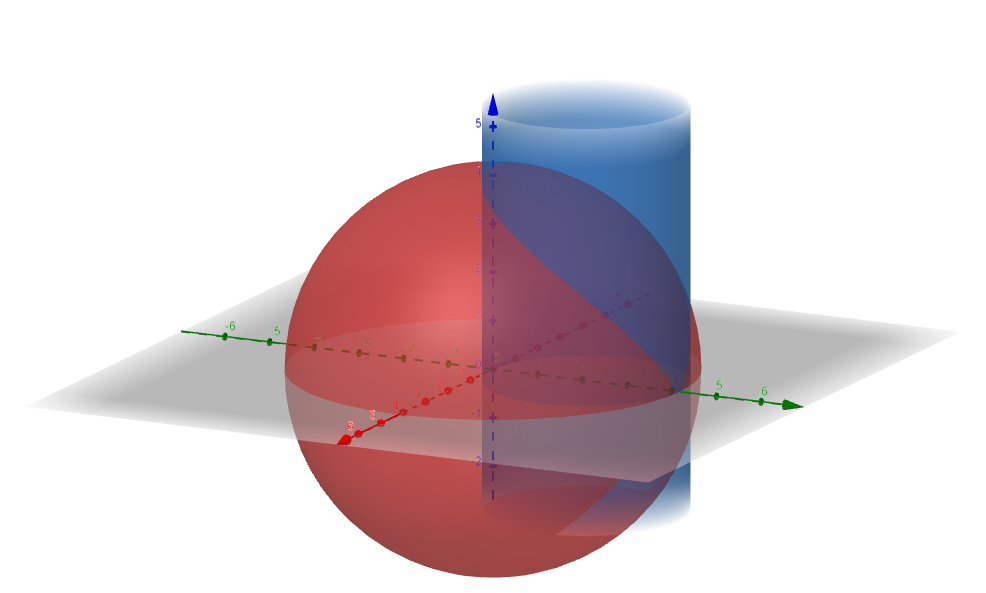
\includegraphics[scale=0.20]{Cone and Sphere}
\end{center}

Vemos que si tomamos coordenadas polares: $r = a\sen \theta$ y además se cumple que:
$$x^2 + y^2 - ay = 0 \Leftrightarrow x^2 + \left(y - \frac{a}{2}\right)^2 = \frac{a^2}{4}$$
Por lo que, considerando $D = \{\left(x, y\right): x^2 + y^2 \le ay\} = \{\left(x, y\right): x^2 + \left(y - \frac{a}{2}\right)^2 \le \frac{a^2}{4}\}$ que es la superficie de la base del cilindro, podemos calcular el volumen como: 
$$vol = 2 \int_{D} \sqrt{a^2 - x^2 - y^2} \dif{x} \dif{y} = $$
$$= 2 \int_{\theta = 0}^{\theta = \pi} \int_{r = 0}^{r = a\sen \theta } r \sqrt{a^2 - r^2} \dif{r} \dif{\theta} = 2 \int_{\theta = 0}^{\theta = \pi} \left[-\frac{1}{3} \left(a^2 - r^2 \right)^{3/2}\right]_{r = 0}^{r = a\sen \theta }\dif{\theta} = $$
$$= \frac{2}{3} \int_{\theta = 0}^{\theta = \pi} a^3 - a^3 \lvert \cos \theta  \rvert^3 \dif{\theta } = \frac{4}{3} \int_{\theta = 0}^{\theta = \frac{\pi}{2}} a^3 - a^3 \cos^3 \theta \dif{\theta } = \ldots = \boxed{\frac{4}{3}a^3 \left(\frac{\pi}{2} - \frac{2}{3}\right)} $$
\end{ej}

\chapter{CÁLCULO VECTORIAL}
Hasta ahora hemos trabajado siempre con funciones cuyo espacio de llegada era $\mathbb{R}$ y se ha hecho todo un trabajo de cimentación de la teoría de la integración para la nueva definición de Lebesque de la integral. A partir de aquí, se van a dar unas nociones de Cálculo Vectorial, esto es, propiedades de dicha definición de integral para funciones cuyo espacio de llegada es $\mathbb{R}^n$.

\section{INTEGRAL DE LÍNEA}
En esta sección, vamos a estudiar como concepto central la integral de línea. Por un lado, para funciones cuyo espacio de llegada es $\mathbb{R} $ puede surgir la pregunta de ¿qué pasa si yo quiero integrar la función en una línea (no necesariamente recta) del plano? Esto calcularía el área bajo la función y sobre dicha línea. Por otro lado, también es razonable pensar qué significa dicha integral si el espacio de llegada es $\mathbb{R}^n$.

\subsection{Definición de curva}
Para poder desarrollar la pregunta hecha al principio de la sección, es necesario primero definir cómo y qué propiedades tiene esa línea o curva sobre la que vamos a integrar.

\begin{defi}
Definimos como \textbf{curva en $\mathbb{R}^n$} a una función $\gamma: \left[ a, b \right] \rightarrow \mathbb{R}^n$ continua y $C^{1)}$ a trozos. En definitiva estamos expresando que:
$$DIUBUJO$$
\end{defi}

\begin{ej}
\begin{enumerate}
    \item Sea $x, y \in \mathbb{R}^n$, podemos definir su envoltura convexa como: 
    $$\left[ x, y \right] = \{ty + \left( 1 - t \right) x: t \in \left[ 0, 1 \right]\} = C_0 \{x, y\}$$
    Esta curva se puede parametrizar de forma que:
    $$\gamma: \left[ 0, 1 \right] \rightarrow\mathbb{R}^n$$
    $$\gamma \left( t \right) = ty + \left( 1 - t \right) x$$
    \item Sea $\gamma: \left[ 0, 2\pi \right] \rightarrow \mathbb{R}^2$, tal que: $\gamma\left( t \right) = \left( \cos t, \sen t \right) $
    $$\begin{tikzpicture}[paths/.style={->, thick, >=stealth'}]


 \node (species_2) at (0,0) 
     {$\gamma(\frac{\pi}{2})$};

 \node (species_3) at (2,-2) 
     {$\gamma(0)=\gamma(2\pi)$};

 \node (species_4) at (0,-4) 
     {$\gamma(\frac{3\pi}{2})$};

 \node (species_5) at (-2,-2) 
     {$\gamma(\pi)$};



 \draw [paths] (species_3) to [bend right=40] node {} (species_2);
 \draw [paths] (species_4) to [bend right=40] node {} (species_3);
 \draw [paths] (species_5) to [bend right=40] node {} (species_4);
 \draw [paths] (species_2) to [bend right=40] node {} (species_5);


 \end{tikzpicture}$$
    \item Sea $\gamma: \left[ 0, \pi \right] \rightarrow \mathbb{R}^2$, tal que $\gamma\left( t \right) = \left( \cos 2t, \sen 2t \right)$
        $$\begin{tikzpicture}[paths/.style={->, thick, >=stealth'}]


 \node (species_2) at (0,0) 
     {$\gamma(\frac{\pi}{4})$};

 \node (species_3) at (2,-2) 
     {$\gamma(0)=\gamma(\pi)$};

 \node (species_4) at (0,-4) 
     {$\gamma(\frac{3\pi}{4})$};

 \node (species_5) at (-2,-2) 
     {$\gamma(\frac{\pi}{4})$};



 \draw [paths] (species_3) to [bend right=40] node {} (species_2);
 \draw [paths] (species_4) to [bend right=40] node {} (species_3);
 \draw [paths] (species_5) to [bend right=40] node {} (species_4);
 \draw [paths] (species_2) to [bend right=40] node {} (species_5);


 \end{tikzpicture}$$
 Misma curva que 2 pero tardo la mitad en recorrerla.
    \item Sea $\gamma \left[ 0, 2\pi \right] \rightarrow \mathbb{R}^2$, tal que $\gamma \left( t \right) = \left( \cos 2t, \sen 2t \right)$
        $$\begin{tikzpicture}[paths/.style={->, thick, >=stealth'}]


 \node (species_2) at (0,0) 
     {$\gamma(\frac{\pi}{4})$};

 \node (species_3) at (2,-2) 
     {$\gamma(0)=\gamma(\pi)=\gamma(2\pi)$};

 \node (species_4) at (0,-4) 
     {$\gamma(\frac{3\pi}{4})$};

 \node (species_5) at (-2,-2) 
     {$\gamma(\frac{\pi}{4})$};



 \draw [paths] (species_3) to [bend right=40] node {} (species_2);
 \draw [paths] (species_4) to [bend right=40] node {} (species_3);
 \draw [paths] (species_5) to [bend right=40] node {} (species_4);
 \draw [paths] (species_2) to [bend right=40] node {} (species_5);


 \end{tikzpicture}$$
 Misma curva que 3 pero la recorro 2 veces.
    \item Sea $\gamma \left[ 0, 2\pi \right] \rightarrow \mathbb{R}^2$, tal que $\gamma \left( t \right) = \left( \cos t, -\sen t \right) $
        $$\begin{tikzpicture}[paths/.style={->, thick, >=stealth'}]


 \node (species_2) at (0,0) 
     {$\gamma(\frac{3\pi}{2})$};

 \node (species_3) at (2,-2) 
     {$\gamma(0)=\gamma(2\pi)$};

 \node (species_4) at (0,-4) 
     {$\gamma(\frac{\pi}{2})$};

 \node (species_5) at (-2,-2) 
     {$\gamma(\pi)$};



 \draw [paths] (species_2) to [bend left=40] node {} (species_3);
 \draw [paths] (species_3) to [bend left=40] node {} (species_4);
 \draw [paths] (species_4) to [bend left=40] node {} (species_5);
 \draw [paths] (species_5) to [bend left=40] node {} (species_2);


 \end{tikzpicture}$$
 Misma curva que 2 pero la recorro en sentido contrario.
\end{enumerate}
A pesar de que los cuatro últimos ejemplos tuviesen la misma apariencia, como curva son elementos distintos puesto que importa el sentido de recorrido de la curva, la velocidad a la que se recorre y el número de veces que se recorre.
\end{ej}

\begin{obs}
Geometricamente, $\gamma'\left( t \right) \in \mathbb{R}^n$ es el vector tangente de la curva en un determinado punto que apunta en la dirección del movimiento.
\end{obs}

\begin{defi}[Velocidad de una Curva]
Sea $\gamma:[a,b]\rightarrow \mathbb{R}^n$ una curva, definimos la \textbf{velocidad} de la misma como: 
$$v = \lvert \lvert \gamma'\left( t \right) \rvert \rvert$$
Que de forma intuitiva, representa el módulo del vector tangente a la curva en ese punto.
\end{defi}

\begin{obs}
La condición de $C^{1)}$ a trozos permite que las curvas puedan poseer ``picos'', es decir, que haya puntos donde la derivada no sea continua o donde no sea derivable, por ejemplo: 
$$\gamma: \left[ -1, 1 \right] \rightarrow \mathbb{R}^2$$
$$\gamma \left( t \right) = \left( t^2, t^3 \right) $$
Su derivada será $\gamma'\left( t \right) = \left( 2t, 3t^2 \right)$ y un pico en $0$.
\end{obs}

\begin{defi}[Longitud de una Curva]
Dada una curva $\gamma:[a,b]\rightarrow \mathbb{R}^n$, definimos su \textbf{longitud} como:
$$\ell\left( \gamma \right) = \int_{a}^{b} \lvert \lvert \gamma'\left( t \right) \rvert \rvert \dif{t}$$
Este concepto coincide con la longitud real de la gráfica de la curva, sin embargo no se demuestra por falta de tiempo.
\end{defi}

\begin{ej}
Sea $\gamma\left( t \right) = \left( \cos t, \sen t, \cos 2t, \sen 2t \right) \in \mathbb{R}^4$, donde $t \in \left[ 0, \pi \right]$ vamos a ver que su longitud es:
$$\gamma'\left( t \right) = \left( -\sen t, \cos t, -2\sen 2t, 2\cos 2t\right) \Rightarrow \lvert \lvert \gamma'\left( t \right) \rvert \rvert^2 = \sen^2 t + \cos^2 t + 4\sen^2 2t + 4 \cos^2 2t = 5$$
$$\ell \left( t \right) = \int_{0}^{\pi} \sqrt{5} \dif{t} = \pi\sqrt{5} $$
\end{ej}
\begin{ej}
Sea $\gamma: \left[ 0, \pi \right] \rightarrow \mathbb{R}^3$ tal que $\gamma \left( t \right) = \left( t, t\sen t, t \cos t \right) $, entonces podemos calcular su longitud como:
$$\gamma'\left( t \right) = \left( 1, \sen t + t\cos t, \cos t - t \sen t\right) $$
$$\lvert \lvert \gamma'\left( t \right) \rvert \rvert^2 = 1 + \sen^2 t + t^2 \cos^2 t + 2t \sen t \cos t + \cos^2 t + t^2 \sen^2 t - 2t \sen t \cos t = 2 + t^2$$
$$\ell \left( \gamma \right) = \int_{0}^{\pi} \sqrt{t^2 + 2} \dif{t}$$
\end{ej}

\begin{defi}[Curva opuesta]
Dada una curva $\gamma:[a,b]\rightarrow \mathbb{R}^n$, definimos su \textbf{curva opuesta}, que denotamos por $(-\gamma):[-b,-a]\rightarrow \mathbb{R}^n$, como: 
$$\left( -\gamma \right) \left( t \right) = \gamma \left( -t \right) $$
Es decir, fundamentalmente son la misma curva, pero cambia el sentido de recorrido.
\end{defi}

\begin{prop}
Sea $\gamma:[a,b]\rightarrow \mathbb{R}^n$ una curva y $-\gamma:[-b,-a]\rightarrow \mathbb{R}^n$ su opuesta, entonces: 
$$\ell \left( -\gamma \right) = \ell \left( \gamma \right) $$
\end{prop}

\begin{defi}[Unión de curvas]
Sea dos curvas $\gamma : \left[ a, b \right] \rightarrow \mathbb{R}^n$ y $\sigma : \left[ b, c \right] \rightarrow \mathbb{R}^m$ tal que $\gamma\left( b \right) = \sigma \left( b \right)$, definimos como la \textbf{curva unión} de ambas a la curva $\gamma \lor \sigma: \left[ a, c \right] \rightarrow \mathbb{R}^n$ definida como:
$$\left( \gamma \lor \sigma \right) \left( t \right) = \begin{cases}
    \gamma\left( t \right) \text{, si } t \in \left[ a, b \right]\\
    \sigma\left( t \right) \text{, si } t \in \left[ b, c \right] 
\end{cases}$$
\end{defi}
\begin{prop}
Sea dos curvas $\gamma : \left[ a, b \right] \rightarrow \mathbb{R}^n$ y $\sigma : \left[ b, c \right] \rightarrow \mathbb{R}^m$ tal que $\gamma\left( b \right) = \sigma \left( b \right)$, entonces:
$$\ell \left( \gamma \lor \sigma \right) = \ell \left( \gamma \right) + \ell\left( \sigma \right) $$
\end{prop}

\begin{defi}[Reparametrización]
Sea $\gamma: \left[ a, b \right] \rightarrow \mathbb{R}^n$ una curva y $h: \left[ a', b' \right] \rightarrow \left[ a, b \right]$ una función creciente, biyectiva y $C^1$ a trozos, entonces llamamos \textbf{reparametrización} de $\gamma$ a:
$$\gamma \circ h: \left[ a', b' \right] \rightarrow \mathbb{R}^n.$$
\end{defi}

\begin{prop}
Sea $\gamma: \left[ a, b \right] \rightarrow \mathbb{R}^n$ una curva y $h: \left[ a', b' \right] \rightarrow \left[ a, b \right]$ que verifican las condiciones de reparametrización de $\gamma$, entonces se conserva la longitud de la curva: 
$$\ell \left( \gamma \circ h \right) = \ell \left( \gamma \right) $$
Intuitivamente una forma alternativa de describir la curva no puede cambiar la longitud de la misma.
\end{prop}
\begin{demo}
$$\ell \left( \gamma \circ h\right) = \int_{a'}^{b'} \lvert \lvert \left( \gamma \circ h \right)'\left( t \right) \rvert \rvert \dif{t} =  \int_{a'}^{b'} \lvert \lvert \gamma'\left( h\left( t \right) \right) h'\left( t \right) \rvert \rvert \dif{t} = \int_{a'}^{b'} h'\left( t \right) \lvert \lvert \gamma'\left( h\left( t \right) \right) \rvert \rvert \dif{t} = $$
$$= \int_{a}^{b} \lvert \lvert \gamma'\left( s \right) \rvert \rvert \dif{s} = \ell \left( \gamma \right) $$    
\end{demo}

\begin{obs}
La reparametrización de una curva conserva la forma, el sentido y la longitud de la curva, pero NO la velocidad de la misma ni aunque los segmentos $[a,b]$ y $[a',b']$ midan lo mismo pues en este caso el tiempo total en completar el recorrido sería el mismo, pero la velocidad puntual en cada punto no.
\end{obs}

\subsection{Concepto de Integral de Línea}
Una vez restringido el significado de lo que es una curva y analizadas sus propiedades con respecto a integral, desarrollamos el concepto de integral de línea.

\begin{defi}[Integral sobre la curva]
Sea $\gamma: \left[ a, b \right] \rightarrow \mathbb{R}^n$ una curva donde $\img \gamma \subset \Omega$ abierto y $f: \Omega \rightarrow \mathbb{R}$ una función continua, entonces la integral sobre la curva es:
\[
\int_{\gamma} f \dif{s} = \int_{a}^{b} \left( f \circ \gamma \right) \left( t \right) \lvert \lvert \gamma'\left( t \right) \rvert \rvert \dif{t} 
\]
\end{defi}

\begin{obs}
Sea $\gamma$ una curva y $f$ una función continua, entonces es sencillo ver que: 
\begin{itemize}
    \item $\ell \left( \gamma \right) = \int_{\gamma} 1 \cdot \dif{s}$
    \item $\int_{\gamma} f \dif{s} = \int_{-\gamma} f \dif{s}$
    \item $\int_{\gamma \lor \sigma} f \dif{s} = \int_{\gamma} f \dif{s} + \int_{\sigma} f \dif{s}$
\end{itemize}
\end{obs}

\begin{defi}[Integral de Línea]
Sea $\gamma: \left[ a, b \right] \rightarrow G \subset \mathbb{R}^n$ una curva, $F: G \rightarrow \mathbb{R}^n$ un campo vectorial\footnote{Este término simplemente indica que es una función entre espacios de la misma dimensión} continuo y el conjunto $G$ abierto, entonces llamamos \textbf{integral de línea} de $F$ sobre $\gamma$ a:
$$\int_{\gamma} F \cdot \dif{\overline{s}} = \int_{a}^{b} F\left( \gamma\left( t \right) \right) \cdot \gamma'\left( t \right) \dif{t}$$
\end{defi}

\begin{prop}
\begin{enumerate}
   	\item Tenemos que si $\sigma$ es una reparametrización de $\gamma$, entonces: 
    $$\int_{\sigma} F \cdot \dif{\overline{s}} = \int_{\gamma} F\cdot \dif{\overline{s}}$$

    \item Del mismo modo, si $-\gamma$ es la curva opuesta a $\gamma$, entonces: 
    $$\int_{-\left( \gamma \right)} F \cdot \dif{\overline{s}} = -\int_{\gamma} F \cdot \dif{\overline{s}}$$
\end{enumerate}
\end{prop}

\begin{obs}
La interpretación geométrica de lo que estamos haciendo es la siguiente:
$$DIBUJO$$
Realmente en la integral de línea lo que haces es calcular las proyecciones sobre la curva de los vectores del campo en cada punto. De esta forma, sumamos los módulos de dichos vectores a lo largo de toda la curva:
$$\int_{\gamma} F\cdot \dif{\overline{s}} = \int_{a}^{b} \underbrace{F\left( \gamma\left( t \right) \right) \cdot \frac{\gamma'\left( t \right)}{\lvert \lvert \gamma'\left( t \right) \rvert \rvert} \lvert \lvert}_{\text{proy. sobre la tangente}} \gamma'\left( t \right) \rvert \rvert \dif{t} = \int_{a}^{b} F_T \left( \gamma\left( t \right) \right) \cdot \lvert \lvert \gamma'\left( t \right) \rvert \rvert \dif{t} = \int_{\gamma} F_T \dif{s}$$
Es sencillo ver que $F(\gamma(t))$ es el vector del campo en el punto $\gamma(t)$ y al multiplicarlo por el cociente siguiente, estamos proyectándolo sobre el vector unitario de la dirección tangente.
\end{obs}

\begin{defi}[Campo conservativo y potencial]
Decimos que un campo $F:G\subset \mathbb{R}^n\rightarrow \mathbb{R}^n$ \textbf{deriva de un potencial} si: 
$$\exists f: G \rightarrow \mathbb{R} \text{ de modo que } F = \nabla f$$
Del mismo modo, decimos que un campo es \textbf{conservativo} si: 
$$\forall \gamma \text{ cerrada }:\int_{\gamma} F\cdot \dif{\overline{s}} = 0$$
\end{defi}

\begin{prop}
Sea $G \subset \mathbb{R}^n$ abierto y $F: G \rightarrow \mathbb{R}^n$ campo vectorial continuo, entonces $F$ deriva de un potencia si y sólo si es conservativo.
\end{prop}
\begin{demo}
\begin{itemize}
\item $\Rightarrow$
$$\int_{\gamma} F\cdot \dif{\overline{s}} = \int_{a}^{b} \nabla f\left( \gamma\left( t \right) \right) \cdot \gamma'\left( t \right) \dif{t} = \int_{a}^{b} \left( f \circ \gamma \right)'\left( t \right) \dif{t} = \left( f \circ \gamma \right)\left( b \right) - \left( f \circ \gamma \right) \left( a \right)$$
Si la curva es cerrada, entonces $\gamma(a) = \gamma(b)$, luego $\left( f \circ \gamma \right)\left( b \right) - \left( f \circ \gamma \right) \left( a \right) = 0$.

\item $\Leftarrow$

Para entender el argumento de la demostración utilizamos como guía el siguiente dibujo:
$$DIBUJO$$
Es decir, cualquier curva cerrada $\gamma$ la podemos dividir como $\gamma_1 \vee -\gamma_2$ y además vemos que:
$$0 = \int_{\gamma_1 \lor \left( -\gamma_2 \right)} F \dif{\overline{s}} = \int_{\gamma_1} F \cdot \dif{\overline{s}} - \int_{\gamma_2} F \cdot \dif{\overline{s}} \Rightarrow \int_{\gamma_1} F \cdot \dif{\overline{s}} = \int_{\gamma_2} F \cdot \dif{\overline{s}}$$
Por razones topológicas, podemos suponer que $G$ es conexo (puesto que cualquier abierto es suma de conexos) y como además $G$ es abierto, entonces es conexo por caminos, es decir, $\forall x \in G: \exists \gamma_x$ que une $x_0$ con $x$.

Definimos la función $f: G \rightarrow \mathbb{R}$ de forma que $f\left( x \right) = \int_{\gamma_x} F \cdot \dif{\overline{s}}$ y para terminar la demostración bastaría con probar que $\nabla f = F$.
Por ser el campo continuo, sabemos que:
$$\forall \varepsilon > 0,\ \exists \delta > 0: \lvert \lvert F\left( x + h \right) - F\left( x \right) \rvert \rvert < \varepsilon \text{ si } \lvert \lvert h \rvert \rvert < \delta$$
Y sabiendo esto escogemos el $\delta$ de forma que $B\left( x, \delta \right) \subset G$ de modo que $x+h \in B(x,\delta)$ y como la bola es convexa, entonces el segmento que denotaremos por $\sigma_n \sim \left[ x, x + h \right]$ pertenece a la bola. Por tanto:
$$\int_{\gamma_x} F\cdot \dif{\overline{s}} + \int_{\sigma_n} F \cdot \dif{\overline{s}} = \int_{\gamma_x \lor \sigma_n} F \dif{\overline{s}} = \int_{\gamma_{x + h}} F \cdot \dif{\overline{s}}$$
Por otro lado, tenemos que:
$$f\left( x + h \right) - f\left( x \right) = \int_{\sigma_n} F \cdot \dif{\overline{s}} = \int_{0}^{1} \left( F\left( x + th \right) \cdot h \right) \dif{t}$$
Luego, entonces:
$$\left\lvert f\left( x + h \right) - f\left( x \right) - F\left( x \right) \cdot h \right\rvert = \left\lvert \int_{0}^{1} F\left( x + th \right) \cdot h \dif{t} - \int_{0}^{1} \left( F\left( x \right) \cdot h\right) \dif{t} \right\rvert$$
$$\left\lvert \int_{0}^{1} \left( F\left( x + th \right) - F\left( x \right) \right) \cdot h \dif{t} \right\rvert \underbrace{\le}_{\text{D.C-S}} \int_{0}^{1} \lvert \lvert F\left( x + th \right) - F\left( x \right) \rvert \rvert \cdot \lVert h \rVert \dif{t} < \varepsilon \lvert \lvert h \rvert \rvert$$
Por tanto, 
$$\left\lvert \frac{f\left( x + h \right) - f\left( x \right) - F\left( x \right) \cdot h}{\lvert \lvert h \rvert \rvert} \right\rvert < \varepsilon$$
Es decir, 
$$\lim_{h \rightarrow 0} \frac{f\left( x + h \right) - f\left( x \right) - \left( F\left( x \right) \cdot h \right)}{\lvert \lvert h \rvert \rvert} = 0 \Rightarrow F\left( x \right) = \nabla f\left( x \right) $$
\end{itemize}
\end{demo}

\begin{theo}[Fórmula de Green]
Sea $G \subset \mathbb{R}^2$ un abierto, $P, Q: G \rightarrow \mathbb{R}$ dos funciones $C^1$ y $D$ un abierto tal que $\overline{D} \subset G$ y donde $\partial D^+ \subset G$ es una curva cerrada, entonces:
$$\int_{\partial D^+} (P, Q) \dif{\bar{s}} = \iint_{D} \left( \frac{\partial Q}{\partial x} - \frac{\partial P}{\partial y} \right) \dif{x} \dif{y}$$
\end{theo}
\begin{demo}
La demostración se va a hacer para conjuntos definidos entre funciones puesto que se puede aproximar cualquier conjunto por una poligonal suficientemente semejante al mismo, cualquier poligonal se puede poner como unión de triángulos y los triángulos son conjuntos de este tipo.

Sea $D = \{\left( x, y \right) : x \in \left[ a, b \right] \; \land \; f\left( x \right) \le y \le g\left( x \right) \}$ con $f, g: \left[ a, b \right] \rightarrow \mathbb{R}$ en $C^1$ a trozos (continuas).
$$\begin{tikzpicture}

\begin{axis}[
tick style={draw=none},
axis y line=middle,
axis x line=middle,
%xlabel=$x$,
%grid = both, %major/minor
xticklabels={},yticklabels={}
];

\addplot [middlearrow={latex reversed},domain=0.98:3, samples=100, name path=f, thick, color=blue!50]
        {sqrt(-x+4) + 1};

\addplot [middlearrow={latex},domain=1:3.02, samples=100, name path=g, thick, color=blue!50]
        {0.7*sqrt(-x+4) + 1};
   
   \addplot [domain=0.98:3, samples=100, name path=f, thick, color=blue!50]
        {sqrt(-x+4) + 1};

\addplot [domain=1:3.02, samples=100, name path=g, thick, color=blue!50]
        {0.7*sqrt(-x+4) + 1};

\addplot[blue!10, opacity=0.4] fill between [of=f and g, soft clip={domain=1:3}];

\draw [middlearrow={latex}, thick, red] (1,2.73) -- (1,2.21);\\
\draw [middlearrow={latex reversed}, thick, red] (3,2) -- (3,1.7);


\draw [dashed] (1,0) -- (1,2.21);
\draw [dashed] (3,0) -- (3,1.7);
\node (n4) [blue] at (2,1.9) {$\sigma_1$};
\node (n3) [blue] at (2,2.35) {$\sigma_2$};
\node (n2) [red] at (2.9,1.9) {$\gamma_1$};
\node (n1) [red] at (1.1,2.5) {$\gamma_2$};

\node (n5) at (1.09,1.72) {$a$};
\node (n6)  at (2.85,1.72) {$b$};


\end{axis}
\end{tikzpicture}$$
Calculamos, las distintas integrales sobre cada curva:
\begin{itemize}
\item  
$$\int_{\substack{\gamma_i\\ i = 1, 2}} P \dif{x} = \int_{\gamma_i} \left( P, 0 \right) \dif{\overline{s}} = 0$$
\item $\sigma_1 \left( t \right) = \left( t, f\left( x \right) \right)$: 
$$\int_{\sigma_1} P \dif{x} = \int_{\sigma_1} \left( P, 0 \right) \dif{s} = \int_{a}^{b} \left( P \left( t, f\left( t \right) \right) \right) \cdot \left( 1, f'\left( t \right) \right) \dif{t} = \int_{a}^{b} P\left( t, f\left( t \right) \right) \dif{t}$$
\item
$$\int_{\sigma_2} P \dif{x} = - \int_{-\sigma_2} P \dif{x} = - \int_{a}^{b} P\left( t, g\left( t \right) \right) \dif{t}$$
\end{itemize}
Por tanto, sobre la integral del enunciado tenemos: 
$$\int_{\partial D^+} P \dif{x} = - \left( \int_{a}^{b} P\left( t, g\left( t \right) \right) \dif{t} - \int_{a}^{b} P\left( t, f\left( t \right) \right) \dif{t} \right) = $$
$$= - \int_{a}^{b} \left( \int_{f\left( x \right)}^{g\left( x \right)} \frac{\partial P\left( x, y \right)}{\partial y} \dif{y} \right) \dif{x} \underbrace{=}_{\text{T. Fubini}} - \iint_{D} \frac{\partial P}{\partial y} \left( x, y \right) \dif{x} \dif{y}$$
Suponiendo ahora las funciones sobre $y$ que definen al conjunto, es decir, $D = \left( x, y \right) : y \in \left[ c, d \right] \; \land \; f\left( y \right) \le x \le g\left( y \right)$ donde $f, g: \left[ c, d \right] \rightarrow \mathbb{R}$ son $C^1$ a trozos. La demostración es completamente análoga: 
$$\int_{\partial D^+} Q \dif{y} \overbrace{=}^{\text{ejercicio}} \iint_{D} \frac{\partial D}{\partial x} \dif{x} \dif{y}$$
Por último, si sumamos las dos fórmulas: 
$$\iint_{\partial D^+} P \dif{x} + Q \dif{y} = \iint_{D} \left( \frac{\partial Q}{\partial x} - \frac{\partial P}{\partial y} \right) \dif{x} \dif{y}$$
\end{demo}

\begin{obs}
En ciertos contextos y suponiendo que tenemos las funciones $P, Q: G \rightarrow \mathbb{R}$, es habitual encontrar el siguiente cambio de notación:
$$\int_{\partial D^+} P \dif{x} + Q \dif{y} = \int_{\partial D^+} (P, Q) \dif{\bar{s}}$$
\end{obs}

\begin{prop}[Fórmula del área]
Sea $D$ un conjunto en las condiciones de la Fórmula de Green, entonces podemos calcular su área como:
$$A\left(D\right)=\iint_{D} \dif{x} \dif{y} = \frac{1}{2}\int_{\partial D^+} x \dif{y} - y \dif{x}$$
\end{prop}
\begin{demo}
Si escogemos $Q\left( x, y \right) = x$ y $P\left( x, y \right) = -y$, por el Teorema anterior tendremos que:
$$\int_{\partial D^+} x \dif{y} - y \dif{x} = 2\iint_{D} \dif{x} \dif{y} = 2 A\left(D\right)$$
\end{demo}

\section{INTEGRAL DE SUPERFICIE}
De nuevo, hemos calculado integrales de funciones cuyo espacio de llegada era $\mathbb{R}$ en conjuntos definidos en $\mathbb{R}^2$. Sin embargo, ¿qué ocurre si el conjunto de integración no es plano sobre $\mathbb{R}^2$ si no que puede ser considerado una superficie en $\mathbb{R}^3$? Además, ¿qué estamos haciendo y cómo si el espacio de llegada es $\mathbb{R}^n$?

\subsection{Concepto de Integral de Superficie}
Para poder responder a las preguntas previas es necesario, de nuevo, acotar el concepto de superficie y ver qué propiedades tiene dicha definición con respecto al concepto de integral.

\begin{defi}[Superficie]
Sea $D \subset  \mathbb{R}^2$ abierto y $\Phi: D \rightarrow \mathbb{R}^3$ una función $C^1$ tal que $\forall \left( u, v \right) \in D : rg\left(D\Phi\left( u, v \right) \right)= 2$, definimos una \textbf{superficie paramétrica} como: 
$$\Phi\left( D \right) = S$$
\end{defi}

\begin{obs}
$$\begin{tikzpicture}
\begin{axis}[
tick style={draw=none},
axis y line=middle,
axis x line=middle,
xticklabels={},yticklabels={}
%grid = both, %major/minor
];
\addplot [thick, domain=-1:8, opacity=0.6]  plot[smooth, tension=.7] coordinates {(2,2.5) (3,3) (4,2.8) (5.2,2.5) (5.5,1.5) (7,0) (6,-2)(4.5,-2.5) (2,-2) (3.5,0.5) (1,1) (2,2.5)};
   

\end{axis}
\node[color=black,right] at (3.5,3.5) {$D$};
\end{tikzpicture}$$
Aplicando $\Phi$  a $D$ obtenemos la superficie paramétrica $S$
$$
\begin{tikzpicture}[x={(170:1cm)},y={(55:.7cm)},z={(90:1cm)}]
  \draw [red] (2.5,-2.5,0) -- (2.5,2.5,0) -- (-2.5,2.5,0) -- (-2.5,-2.5,0) -- cycle;
  \draw[dashed,looseness=.6] (2.5,-2.5,-1) node[above right] {$S$}
  to[bend left] (2.5,2.5,-1)
  to[bend left] coordinate (mp) (-2.5,2.5,-1)
  to[bend right] (-2.5,-2.5,-1)
  to[bend right] coordinate (mm) (2.5,-2.5,-1)
  -- cycle;
  \draw[dashed,looseness=.2] (mm) to[bend left] (0,0,0) to[bend left] (mp);


  \draw[->] (0,0,0) -- (3,0,0) node[left] {$\Phi (u,v)$};
  \draw[->] (0,0,0) -- (0,3,0) node[above right] {$\Phi_v (u,v)$};
  \draw[->] (0,0,0) -- coordinate[pos=.3] (psi) (1,0,2) node[above left] {$\Phi_u (u,v)$};


\end{tikzpicture}$$
Intuitivamente, estamos diciendo que escogemos un trozo del plano en $\mathbb{R}^2$, lo metemos en $\mathbb{R}^3$ y lo moldeamos como queramos para formar nuestra superficie.

Por la definición que se ha dado, podemos expresar la diferencial como: 
$$\begin{pmatrix} \frac{\partial \Phi_1}{\partial u} & \frac{\partial \Phi_1}{\partial v} \\
\frac{\partial \Phi_2}{\partial u} & \frac{\partial \Phi_2}{\partial v} \\ 
\frac{\partial \Phi_3}{\partial u} & \frac{\partial \Phi_3}{\partial v} \end{pmatrix} = \begin{pmatrix} \frac{\partial \Phi}{\partial u} & \frac{\partial \Phi}{\partial v} \end{pmatrix} $$
donde las parciales generales sobre $u$ y $v$ son las tangentes sobre la recta en su respectiva coordenada. Precisamente por esto, el espacio generado por $\left\langle \Phi_u, \Phi_v\right\rangle$ es un plano paralelo al tangente a la superficie en ese punto, puesto que los tangentes anteriores son independientes y conforman un sistema generador. El que es realmente será tangente a la superficie es: 
$$\boxed{\Phi \left( u, v \right) + \img D \Phi \left( u, v \right)}$$
Y, por tanto, es razonable pensar que el vector $\frac{\partial\Phi}{\partial u} \times \frac{\partial\Phi}{\partial v}$ será perpendicular a la superficie, por ser perpendicular al plano tangente a la misma.
\end{obs}

\underline{Notación}

A partir de ahora y durante el resto del documento, se utilizarán las siguientes expresiones:
\begin{align*}
\Phi_u = \frac{\partial \Phi}{\partial u} & & \Phi_v = \frac{\partial \Phi}{\partial v}
\end{align*}
para simplificar la complejidad de las expresiones.

\begin{defi}[Área de una superficie]
Dada una superficie $S$ en términos de la caracterización anterior, definimos el \textbf{área} como: 
$$A\left( S \right) = \iint_{D} \lVert \Phi_{u} \times \Phi_v \rVert \dif{u} \dif{v}$$
Cabe destacar que dicha definición coincide\footnote{La demostración se omite por ser muy extensa} con el concepto geométrico de área de una superficie.
\end{defi}

\begin{ej}
Sea $f: \left[ a, b \right] \rightarrow \mathbb{R}$ de $C^1$ y $\forall x \in \left[ a, b \right]: f\left( x \right) \ge 0$, podemos calcular el área generada por su revolución de la siguiente forma:
$$      \begin{tikzpicture}[scale=1,>=latex,x=1.5cm,y=0.8cm]
        \fill[fill=green,opacity=0.5] (1,0) -- plot[domain=1:4] (\x,{sqrt(2*(\x)+1))}) -- (4,0);
        \fill[fill=green,opacity=0.5] (1,0) -- plot[domain=1:4] (\x,{-sqrt(2*(\x)+1))}) -- (4,0);
        \draw[-,thick,domain=1:4,samples=100] plot (\x,{sqrt(2*(\x)+1))}) node[right] {\footnotesize $f(x)$};
        \draw[-,thick,domain=1:4,samples=100] plot (\x,{-sqrt(2*(\x)+1))});
        \draw[fill=gray!50] (4,0) circle [x radius =.2 , y radius =3];
        \draw[fill=gray!50] (1,0) circle [x radius =.2 , y radius =1.732050808];

        \draw[->,thick] (-1,0) -- (5,0) node[above] {\footnotesize $x$};
        \draw[->,thick] (0,-5) -- (0,5) node[below right]{\footnotesize $y$};
        \draw[-] (1,3pt) -- (1,-3pt) node[below] {\footnotesize $a$};
        \draw[-] (4,3pt) -- (4,-3pt) node[below] {\footnotesize $b$};
   \draw (0.5,0) node {\AxisRotator}; 
    \end{tikzpicture}$$
En primer lugar, es necesario parametrizar dicha superficie:
$$\Phi: \left( a, b \right) \times \left( 0, 2\pi \right) \rightarrow \mathbb{R}^3$$
$$\Phi \left( u, v \right) = \left( u, f\left( u \right)\cos v, f\left( u \right)\sin v \right) $$
Con esta parametrización, solo renunciamos al borde de puntos de $a$ a $b$ y los puntos del plano horizontal, pero como tienen medida nula no influyen en el resultado, ahora: 
$$\begin{cases}
\Phi_u = \left( 1, f'\left( u \right) \cos v, f'\left( u \right) \sin v \right) \\ \Phi_v = \left( 0, -f\left( u \right) \sin v, f\left( u \right) \cos v \right)
\end{cases}\Rightarrow \Phi_u \times \Phi_v = \left( f\left( u \right) f'\left( v \right) \left[ \cos^2 v + \sin^2 v \right], -f\left( u \right) \cos v, -f\left( u \right) \sin v \right)$$
$$\lVert \Phi_u \times \Phi_v \rVert = \sqrt{f\left( u \right)^2 \left[ f'\left( u \right) \right]^2 + f\left( u \right)^2} = f\left( u \right) \sqrt{1 + f'\left( u \right)^2} \Rightarrow$$
$$A\left( S \right) = \int_{a}^{b} \left( \int_{0}^{2\pi} f\left( u \right) \sqrt{1 + f'\left( u \right)^2} \dif{v} \right) \dif{u} = 2\pi \int_{a}^{b} f\left( u \right) \sqrt{1 + f'\left( u \right)^2} \dif{u} $$
Vemos finalmente que la expresión final es, en cierta manera, como integrar las áreas de cada anillo desde $a$ hasta $b$.
\end{ej}

\begin{defi}[Integral sobre una superficie]
Sea $S \subset G \subset \mathbb{R}^3$ donde $G$ es un abierto y $f: G \rightarrow \mathbb{R}$ continua, definimos la \textbf{integral de $f$ sobre $S$} como: 
$$\iint_{S} f \dif{S} = \iint_{D} f\left( \Phi\left( u, v \right) \right) \lVert \Phi_u \times \Phi_v \rVert \dif{u} \dif{v}$$
donde $\Phi: D \rightarrow \mathbb{R}^3$ es la parametrización de $S$.
\end{defi}

\begin{obs}
Si tomamos como $f = 1$, entonces estamos calculando el área de $S$.
\end{obs}

\begin{prop}
Sea $\varphi: G \rightarrow D$ difeomorfismo de $C^1$, entonces: 
$$\Phi \circ \varphi: G \rightarrow S \subset \mathbb{R}^3$$
es una reparametrización.
\end{prop}
\begin{demo}
Tenemos que: 
$$D\left( \Phi \circ \varphi \right) \left( u, v \right) = D\Phi\left( \varphi\left( u, v \right) \right) \circ D\varphi\left( u, v \right)$$
\end{demo}

\begin{prop}
El área de una superficie se mantiene invariante ante reparametrizaciones:
$$\iint_{D} f\left( \left( \Phi \circ \varphi \right) \left( x, y \right) \right) \lVert \left( \Phi \circ \varphi \right)_x \left( \Phi \circ \varphi \right)_y \rVert \dif{x} \dif{y}$$
Este área es la misma puesto que:
$$\lVert \left( \Phi \circ \varphi \right)_x \times \left( \Phi \circ \varphi \right)_y \rVert = \lvert \det D \varphi\left( x, y \right) \rvert \lVert \Phi_u \left( \varphi\left( x, y \right) \right) \times \Phi_v \left( \varphi\left( x, y \right) \right) \rVert$$
\end{prop}

\begin{defi}[Integral de Superficie]
Sea $G \subset \mathbb{R}^3$ un abierto, $S \subset G$ una superficie en él parametrizada por $\Phi: D \rightarrow S$ y $F: G \rightarrow \mathbb{R}^3$ un campo continuo, definimos la \textbf{integral de superficie} de $F$ sobre $S$ a: 
$$\iint_{S} F \dif{\overline{S}} = \iint_{D} F\left( \Phi\left( u, v \right) \right) \cdot \left( \Phi_u \times \Phi_v \right) \dif{u} \dif{v}$$
\end{defi}

\begin{obs}
Del mismo modo que se hizo con las integrales de línea, aquí la idea intuitiva es que $F\left( \Phi\left( u, v \right) \right)$ es el vector que asigna el campo al punto $\Phi\left( u, v \right)$ de la superficie, pues dicho vector se proyecta sobre el vector normal a la superficie en ese punto que es $\Phi_u \times \Phi_v$ y sumamos todos esos vectores. Es decir, si recordamos el producto mixto de vectores, esto es, $a\cdot b\times c$ esta expresión nos daba el volumen del paralelepípedo formado por los 3 vectores, luego de alguna forma estamos sumando los volúmenes generados por un trozo diferencial de superficie.
$$DIBUJO$$
Por tanto, esta integral nos permite calcular el \textbf{flujo} del campo que atraviesa la superficie. Además, es necesario tener en cuenta las siguientes características:
\begin{itemize}
    \item El signo de la integral depende de la parametrización, luego habrá que determinar algún sistema para diferenciar la integral.
    \item Si $F$ es tangente a $S \Rightarrow \iint_{S} F \dif{\overline{S}} = 0$.

Para hacer más patente el significado de la integral de superficie vemos que:
$$\iint_{S} F \dif{\overline{S}} = \iint_{D} F\left( \Phi\left( u, v \right) \right) \cdot \left( \Phi_u \times \Phi_v \right) = \iint_{D} F\left( \Phi\left( u, v \right) \right) \cdot \underbrace{\frac{\Phi_u \times \Phi_v}{\lVert \Phi_u \times \Phi_v \rVert}}_{\vec{n}} \cdot \lVert \Phi_u \times \Phi_v \rVert = \iint_{S} F_{\vec{n}} \dif{S}$$
Es decir, estamos haciendo una integral sobre una superficie de la función que proyecta el campo sobre el vector normal.
\end{itemize}
\end{obs}

\begin{prop}
La integral de superficie es invariante por reparametrizaciones siempre que conserven la orientación. De hecho, en caso de que no la conserven únicamente cambia el signo de la integral.
\end{prop}

\begin{ej}
Sea: 
$$\overline{n} = \frac{\Phi_u \times \Phi_v}{\lVert \Phi_u \times \Phi_v \rVert}$$
y también: 
$$S \rightarrow \mathbb{R}^n,\ p \mapsto \begin{cases}
    \vec{n}_p\\
    -\vec{n}_p
\end{cases} $$
Siempre que se pueda hacer esta ``selección'' de forma continua diremos que la superficie es \textbf{orientable}. En el caso de una esfera, solo habrá dos posibles orientaciones.

Como superficie no orientable tenemos la banda de Möbius.
\begin{center}
    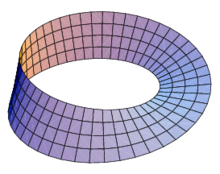
\includegraphics[scale=0.3]{images/mobius} 
\end{center}
\end{ej}

\subsection{Rotacional y Divergencia de un campo}
Se van a desarrollar dos conceptos fundamentales en el análisis vectorial que son la divergencia y el rotacional de un campo. Estos elementos matemáticos son esenciales en áreas como la mecánica de fluidos, la aerodinámica o física y permiten analizar las características que tiene un campo concreto sobre el espacio en el que está definido.

\begin{defi}[Borde de una superficie]
Sea $D$ el recinto interior a una curva $\gamma$ y $\Phi: D \rightarrow \mathbb{R}^3$ la parametrización de una superficie que se puede extender de forma inyectiva y $C^1$ a $\bar{D}$, es decir, a $\partial D$, definimos el \textbf{borde de $S$} como:
$$\partial S = \Phi\left( \partial D \right)$$
$$DIBUJO$$
Esta definición permite trabajar siempre con conjuntos $D$ muy regulares donde $\partial D$ es una curva cerrada cuyo interior es $D$.
\end{defi}
\begin{obs}
Por la definición que se ha dado, tenemos que: 
$$\left[ a, b \right] \xrightarrow{\gamma} \mathbb{R}^2 \xrightarrow{\Phi} \mathbb{R}^3$$
Luego $\Phi \circ \gamma$ parametriza a la curva $\partial S$, por tanto, es razonable pensar qué orientación inducir a dicha curva para que todo se mantenga uniforme (ya hemos visto que la integral depende de la oritentación). Tomemos las siguientes orientaciones: 
    \begin{itemize}
        \item Sabemos la orientación de $S$ a través de $\Phi$. 
        \item Sabemos la orientación de $\gamma$ a través de $D$
    \end{itemize}
Éstas orientaciones determinan una orientación concreta de la curva definida por $\Phi \circ \gamma$. Cuando dada una superficie se toma como orientación de su borde la que viene dada por éste proceso, decimos que la superficie y su borde están orientados de forma compatible.
\end{obs}

\begin{defi}[Rotacional]
Sea el campo $F: \mathbb{R}^3 \rightarrow \mathbb{R}^3$ llamamos \textbf{rotacional} de $F$ a: 
$$\rot F = \nabla \times F = \begin{vmatrix} i & j & k\\
\frac{\partial}{\partial x} & \frac{\partial }{\partial y} & \frac{\partial }{\partial z} \\
F_1 & F_2 & F_3\end{vmatrix} = \left( \frac{\partial F_3}{\partial y} - \frac{\partial F_2}{\partial z}, \frac{\partial F_1}{\partial z} - \frac{\partial F_3}{\partial x}, \frac{\partial F_2}{\partial x} - \frac{\partial F_1}{\partial y} \right)$$
\end{defi}

\begin{obs}
En cierta manera, el rotacional mide la cantidad de giro que provoca el campo en un punto concreto del mismo. Si éste es distinto de 0 hay giro (positivo o negativo determinan el sentido) y si éste es cercano a 0 quiere decir que no hay giro.
\end{obs}

\begin{theo}[de Stokes]
Dada una superficie orientada $S$ con borde orientado de forma compatible y un campo $F$ de clase $C^1$, entonces:
$$\iint_{S} \rot F \dif{\overline{S}} = \int_{\partial S} F \dif{\overline{s}}$$
\end{theo}
\begin{demo}
La demostración se va a hacer para el caso en que la superficie es la gráfica de una función, puesto que es posible demostrar que cualquier superficie se puede poner en términos de otras que sean de esta forma.

Por un lado, la parametrización $\Phi: D \rightarrow \mathbb{R}^3$ de la superficie nos indica que
$$\Phi\left( x, y \right) = \left( x, y, f\left( x, y \right) \right)\Rightarrow \Phi_x \times \Phi_y = \left( \frac{-\partial f}{\partial x}, \frac{-\partial f}{\partial y}, 1\right)$$
la orientación que se toma es hacia las $z$ positivas por ser un 1 la tercera coordenada.

Del mismo modo, tomamos la parametrización $\sigma: I \rightarrow \mathbb{R}^2$ de la curva $\partial D$ de la forma:
$$\sigma\left( t \right) = \left( x\left( t \right), y\left( t \right) \right)$$

Estas dos elecciones, inducen una parametrización en $\partial S$ tal que: 
$$\partial D \xrightarrow{\Phi \circ \sigma} \partial S \stackrel{\Phi \circ \sigma = \gamma}{\Rightarrow} \gamma: I \rightarrow \mathbb{R}^3$$
$$\gamma\left( t \right) = \left( x\left( t \right), y\left( t \right), f\left( x\left( t \right), y\left( t \right) \right) \right)$$

Por tanto, por un lado:
$$\iint_{S} \rot F \dif{\overline{S}} = \int_{D} \rot F \cdot \left( \Phi_x \times \Phi_y \right) \dif{x} \dif{y} =$$
$$= \iint_{D} \left( \left( \frac{\partial F_3}{\partial y} - \frac{\partial F_2}{\partial z} \right) \left( -\frac{\partial f}{\partial x} \right) + \left( \frac{\partial F_1}{\partial z} - \frac{\partial F_3}{\partial x} \right) \left( -\frac{\partial f}{\partial y} \right) + \left( \frac{\partial F_2}{\partial x} - \frac{\partial F_1}{\partial y} \right) \right)$$
Por el otro lado: 
$$\int_{\partial S} F \dif{\overline{s}} = \int_{a}^{b} \left( F_1, F_2, F_3 \right) \cdot \left( x'\left( t \right), y'\left( t \right), \frac{\partial f}{\partial x} x'\left( t \right) + \frac{\partial f}{\partial y} y'\left( t \right) \right) = $$
$$= \int_{a}^{b} \left( F_1x'\left( t \right) - F_2y'\left( t \right) + F_3\left( \frac{\partial f}{\partial x} x'\left( t \right) + \frac{\partial f}{\partial y} y'\left( t \right) \right) \right) \dif{t} = $$
$$= \int_{\partial D} \left( F_1 + F_3 \frac{\partial f}{\partial x} \right) \dif{x} + \left( F_2 + F_3 \frac{\partial f}{\partial y} \right) \dif{y} \stackrel{\text{F. Green}}{=}\iint_{D} \frac{\partial}{\partial x} \left( F_2 + F_3 \frac{\partial f}{\partial y} \right) - \frac{\partial}{\partial y} \left( F_1 + F_3 \frac{\partial f}{\partial x} \right) \dif{x} \dif{y}$$
Y desarrollando se ve que las dos cosas son iguales.
\end{demo}
\begin{obs}
La interpretación geométrica del teorema nos viene de nuevo a remarcar el significado profundo del rotacional: el grado de giro (que viene dado por el rotacional) en un área $S$ es más o menos como:
$$\int_{S} \rot F \dif{\overline{S}} \approx \lVert \rot F \left( p \right) \rVert \cdot Area\left( S \right)$$
pero el teorema dice que se puede calcular también como la integral de línea de $F$ sobre el borde de dicha superficie. Como vimos que la integral de línea era sumar los módulos de las proyecciones del campo sobre las tangentes de la curva, en cierta manera estamos sumando todos los vectores de giro en el borde tal y como muestra el siguiente dibujo:
\begin{center}
    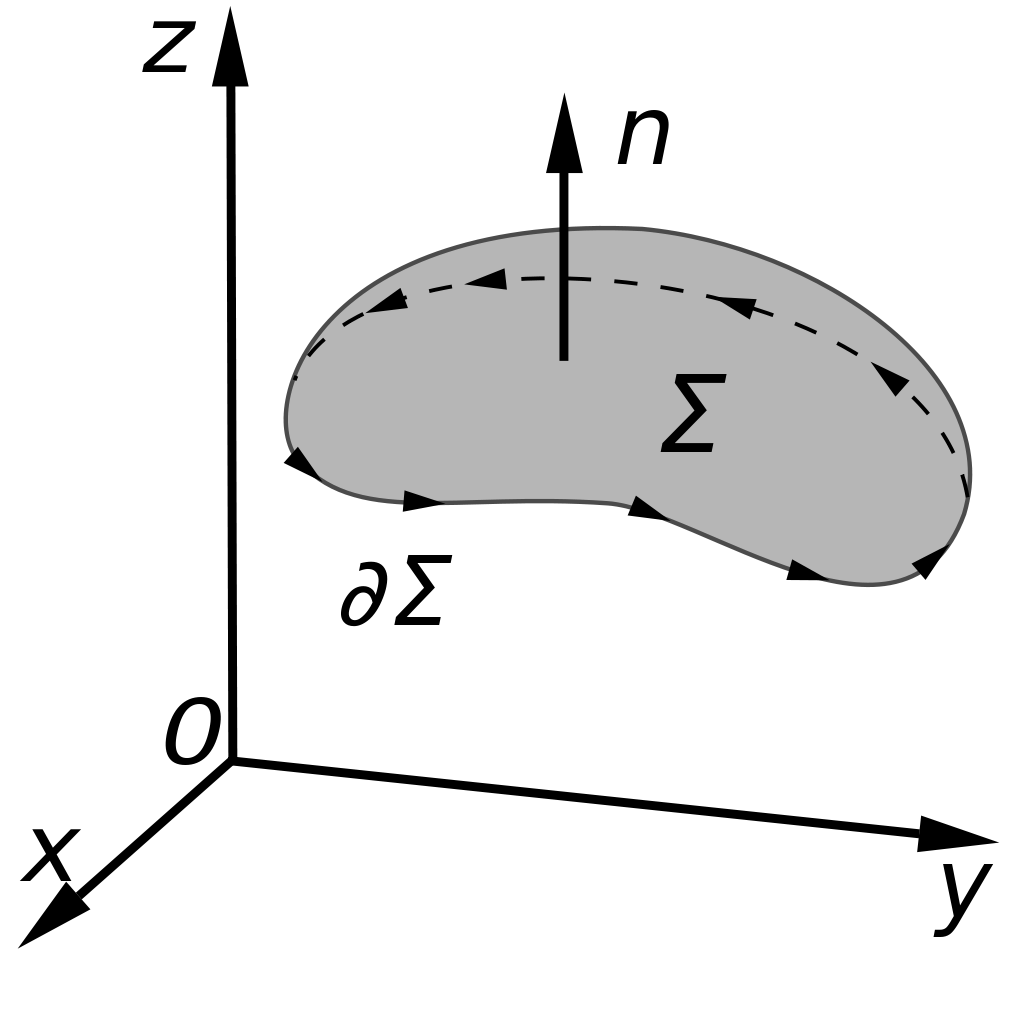
\includegraphics[scale=0.1]{images/stokeTh} 
\end{center}
\end{obs}

\begin{theo}
Sea $F: \mathbb{R}^3 \rightarrow \mathbb{R}^3 \in C^1$. Son equivalentes: 
\begin{itemize}
    \item $F$ es conservativo.
    \item $\exists f: \mathbb{R}^3 \rightarrow \mathbb{R}$ de $C^2$ de modo que $F = \nabla f$ 
    \item $\rot F = 0$
\end{itemize}
\end{theo}
\begin{demo}
La implicación $1)\Rightarrow 2)$ ya la vimos cuando definimos lo que era un campo conservativo, luego sólo faltan las otras.
\begin{itemize}
\item $2) \Rightarrow 3)$

Esta implicación es inmediata porque el Tª de Schwarz nos asegura que las parciales segundas cruzadas son iguales, luego para $F = \left( \frac{\partial f}{\partial x}, \frac{\partial f}{\partial y}, \frac{\partial f}{\partial z} \right)$, tenemos que:
$$\rot F = \begin{vmatrix} \vec{i} & \vec{j} & \vec{k} \\
\frac{\partial }{\partial x} & \frac{\partial }{\partial y} & \frac{\partial }{\partial z} \\
\frac{\partial f}{\partial x} & \frac{\partial f}{\partial y} & \frac{\partial f}{\partial z} \end{vmatrix} \underbrace{=}_{T. Schwarz} \left( 0, 0, 0 \right)$$

\item $3 \Rightarrow 1)$: 
$$DIBUJO$$

Sea $S$, si tomamos $\partial S = \gamma$ como curva, entonces por ser el rotacional nulo y el Teorema de Stokes, sabemos que: 
$$\int_{\gamma} F \dif{\overline{s}} = \iint_{S} \rot F \dif{\overline{S}} = 0$$
La demostración no es del todo rigurosa porque falta demostrar que para una curva cualquiera, existe una superficie de la que es borde y esto es más extenso de demostrar (pero cierto).
\end{itemize}
\end{demo}

\begin{obs}
Precisamente de la última observación se deduce que el resultado NO es cierto si $F$ no tiene dominio en todo $\mathbb{R}^3$ o, si se quiere precisar más, si no tiene dominio en un conjunto simplemente conexo (que no haya tubos infinitos que me agujeren una posible superficie).
\end{obs}

\begin{ej}
Sea $G = \mathbb{R}^3 \setminus Z$ y $F: G \rightarrow \mathbb{R}^3$ con $F\left( x, y, z \right) = \left( \frac{-y}{x^2 + y^2}, \frac{x}{x^2 + y^2}, 0 \right)$, vemos que $\rot F = \left( 0, 0, 0 \right)$ porque trivialmente las dos primeras componentes son 0, pero la tercera componente además:
$$\frac{\partial \left( \frac{x}{x^2 + y^2} \right)}{\partial x} - \frac{\partial \left( \frac{-y}{x^2 + y^2} \right)}{\partial y} = \frac{x^2 + y^2 - 2x^2}{\left( x^2 + y^2 \right)^2} + \frac{x^2 + y^2 - 2y^2}{\left( x^2 + y^2 \right)^2} = 0$$
Tomamos la curva:
$$\gamma: \left[ 0, 2\pi \right] \rightarrow \mathbb{R}^3$$
$$\gamma\left( t \right) = \left( \cos t, \sin t, 0 \right)$$
Y vemos que:
$$\int_{\gamma} F \dif{\overline{s}} = \int_{0}^{2\pi} \left( -\sin t, \cos t, 0 \right) \cdot \left( -\sin t, \cos t, 0 \right) \dif{t} = \int_{0}^{2\pi} \cos^2 t + \sin^2t \dif{x} = 2\pi$$
Este ejemplo hace evidente la necesidad de que el dominio sea $\mathbb{R}^3$ ya que no podemos construir una superficie con la curva formada por la circunferencia unidad que no corte al eje Z.
\end{ej} 

\begin{defi}[Divergencia]
Sea $F: G \rightarrow \mathbb{R}^3$ un campo de $C^1$ y $G \subset \mathbb{R}^3$ un abierto, llamamos \textbf{divergencia} de $F$ a: 
$$\divg F = \frac{\partial F_1}{\partial x} + \frac{\partial F_2}{\partial y} + \frac{\partial F_3}{\partial z} = \nabla \cdot F$$
\end{defi}

\begin{obs}
La idea intuitiva detrás del concepto de la divergencia es la cantidad de flujo que sale o entra en un punto del campo, es decir, que para divergencias cercanas a 0 tendremos puntos donde no hay casi flujo de campo, pero para divergencias lejanas a 0 tendremos puntos donde entra más campo o sale más campo (depende del signo).
\end{obs}

\begin{prop}
Sea $H$ un campo $C^2$, entonces $\divg \left( \rot H \right) = 0$. Luego que la divergencia de un campo sea 0 será condición necesaria para ser el rotacional de algún otro.
\end{prop}
\begin{demo}
De nuevo, por el Teorema de Schwarz para las parciales segundas cruzadas:
$$\left( \underbrace{\frac{\partial H_3}{\partial y} - \frac{\partial H_2}{\partial z}}_{\frac{\partial }{\partial x}}, \underbrace{\frac{\partial H_1}{\partial z} - \frac{\partial H_3}{\partial x}}_{\frac{\partial }{\partial y}}, \underbrace{\frac{\partial H_2}{\partial x} - \frac{\partial H_1}{\partial y}}_{\frac{\partial }{\partial z}} \right) = 0$$
\end{demo}

\begin{theo}
Sea $F: \mathbb{R}^3 \rightarrow \mathbb{R}^3$ un campo de $C^1$ tal que su $\divg F = 0$, entonces $\exists G$ campo de $C^2$ tal que $F = \rot G$.
\end{theo}
\begin{demo}
El $G$ que es rotacional de $F$ viene dado por:
$$\begin{cases}
G_1\left( x, y, z \right) = \displaystyle \int_{0}^{z} F_2\left( x, y, t \right) \dif{t} - \int_{0}^{y} F_3\left( x, t, 0 \right) \dif{t} \\  G_2\left( x, y, z \right) = \displaystyle  -\int_{0}^{z} F_1\left( x, y, t \right) \dif{t} \\ G_3\left( x, y, z \right) = 0
\end{cases}$$
\end{demo}
\begin{obs}
\begin{enumerate}
    \item $G$ no es único, puesto que si tenemos un campo $H$ con $H_3 \neq 0$, entonces $\rot H = F = \rot G \Rightarrow H \neq G$.
    \item El campo gravitatorio es un contraejemplo en el caso de que quitemos un punto del dominio del campo, luego tiene que estar definido en $\mathbb{R}^3$.
\end{enumerate}
\end{obs}

\begin{theo}[de la Divergencia de Gauss]
Sea $\Omega \subset \mathbb{R}^3$ dominio\footnote{Esto quiere decir que $\mathring{\overline{\Omega}} = \mathring{\Omega}$, que $\overline{\Omega} = \overline{\mathring{\Omega}}$ y que $\partial \Omega$ acota a $\Omega$} con la frontera $\partial \Omega$ orientada hacia el exterior y sea $F: G \rightarrow \mathbb{R}^3$ un campo de $C^1$ donde $ \overline{\Omega} \subset G$ y $G$ es un abierto, entonces: 
$$\iint_{\partial \Omega} F \dif{\overline{S}} = \iiint_{\Omega} \divg F$$
$$DIBUJO$$
\end{theo}
\begin{demo}
Vamos a hacer la demostración para el caso en el que suponemos que $\Omega = \left\{ \left( x, y, z \right) : f\left( x, y \right) \le z \le g\left( x, y \right) \right\}$ con $f, g : D \rightarrow \mathbb{R}$ de $C^1$, $D \subset \mathbb{R}^2$ y $f \le g$.
$$DIBUJO$$
Sea $F = \left( F_1, F_2, F_3 \right)$ y $\int_{\Omega} \divg F = \int_{\Omega} \left( \frac{\partial F_1}{\partial x} + \frac{\partial F_2}{\partial y} + \frac{\partial F_3}{\partial z} \right) \dif{x} \dif{y} \dif{z}$. En primer lugar, podemos dividir $\partial \Omega = S_1 \cup S_2 \cup S_3$. 
Luego, tenemos que:
$$\int_{\Omega} \frac{\partial F_3}{\partial z} \dif{x} \dif{y} \dif{z} = \int_{D} \left[ \int_{f\left( x, y \right)}^{g\left( x, y \right)} \frac{\partial F_3}{\partial z} \dif{z} \right] \dif{x} \dif{y} = \int_{D} F_3\left( x, y, g\left( x, y \right) \right) - F_3\left( x, y, f\left( x, y \right) \right) \dif{x} \dif{y}$$
Por el otro lado, tenemos:
$$\iint_{\partial \Omega} \left( 0, 0, F_3 \right) \dif{\overline{S}} = \int_{S_1} \left( 0, 0, F_3 \right) + \iint_{S_2} \left( 0, 0, F_3 \right) + \underbrace{\iint_{S_3} \left( 0, 0, F_3 \right)}_{= 0 \text{ (por pendicularidad)}}$$
Parametrizamos la superficie $S_1$, tomando $\Phi: D \rightarrow \mathbb{R}^3$ tal que $\Phi\left( x, y, f\left( x, y \right) \right)$, luego:
$$\begin{cases}
\Phi_x = \left( 1, 0, \frac{\partial f}{\partial x} \right) \\ \Phi_y = \left( 0, 1, \frac{\partial f}{\partial y} \right)
\end{cases}\Rightarrow \Phi_x \times \Phi_y = \left( -\frac{\partial f}{\partial x}, - \frac{\partial f}{\partial y}, 1 \right)$$
Con esto: 
$$\iint_{S_1} \left( 0, 0, F_3 \right) \dif{\overline{S}} = \int_{S_1} \left[ \left( 0, 0, F_3 \right) \cdot n_1 \right] \dif{S} = \iint_{S_1} F_3\left( x, y, f\left( x, y \right) \right) \cdot \frac{- 1}{\sqrt{1 + \left(\frac{\partial f}{\partial x}\right)^2 + \left(\frac{\partial f}{\partial y}\right)^2}} \dif{S} $$
$$= -\iint_{D} F_3\left( x, y, f\left( x, y \right) \right) \frac{1}{\cancel{\sqrt{1 + \frac{\partial f}{\partial x}^2 + \frac{\partial f}{\partial y}^2}}} \cdot \cancel{\sqrt{1 + \frac{\partial f}{\partial x}^2 + \frac{\partial f}{\partial y}^2}} \dif{S} = - \iint_{D} F_3\left( x, y, f\left( x, y \right) \right) \dif{x} \dif{y}$$
Calculando ahora sobre la superficie $S_2$, tenemos que:
$$\iint_{S_2} \left( 0, 0, F_3 \right) \dif{\overline{S}} = \iint_{D} F_3\left( x, y, g\left( x, y \right) \right) \dif{x} \dif{y}$$
Por tanto, hemos probado que:
$$\int_{\Omega} \frac{\partial F_3}{\partial z} \dif{x} \dif{y} \dif{z} = \iint_{\Omega} \left( 0, 0, F_3 \right) \dif{\overline{S}}$$

(\textit{Dibujo, entre dos gráficas verticales})

De modo completamente análogo y escribiéndolo todo para que sean funciones en el otro eje, tenemos que: 
$$\int_{\Omega} \frac{\partial F_2}{\partial y} \dif{x} \dif{y} \dif{z} = \int_{\partial \Omega} \left( 0, F_2, 0 \right) \dif{\overline{S}} $$

(\textit{Dibujo, entre otras dos gráficas verticales}) 

Y, de nuevo:
$$\int_{\Omega} \frac{\partial F_1}{\partial x} \dif{x} \dif{y} \dif{z} = \int_{\partial \Omega} \left( F_1, 0, 0 \right) \dif{\overline{S}}$$
Consecuentemente, sumando estas últimas ecuaciones obtenemos el resultado del enunciado.
\end{demo}
\begin{obs}
La idea que subyace tras este teorema es que la cantidad de flujo de campo que atraviesa un conjunto $\Omega$ puede expresarse en términos de la divergencia de cada punto de dicho recinto, es decir, como podemos ver aproximado $\iiint_{\Omega} \divg F \dif{x} \dif{y} \dif{z} \approx \divg F\left( p \right) \cdot V\left( \Omega \right)$, entendemos que estamos sumando las divergencias del campo en cada punto de dicho conjunto. El teorema por tanto afirma que calcular eso es lo mismo que calcular el flujo a través de la superficie, que se expresa como $\iint_S F\dif{\overline{S}}$.
\end{obs}

\end{document}
